\documentclass[a4paper,11pt]{article}
\usepackage[utf8]{inputenc}
\usepackage[frenchb]{babel}
\usepackage{numprint}
\usepackage{amssymb}
\usepackage{amsmath}
\usepackage{amsthm}
\usepackage{mathrsfs}
\usepackage{array}
\usepackage{graphicx}
\usepackage{color}
\usepackage{slashbox}
\usepackage{subfigure}
\usepackage{cancel}
\usepackage{verbatim}
\usepackage{multirow}
\usepackage{rotating}
\usepackage[top=2cm]{geometry}
\usepackage{listings}
\usepackage{algorithm2e}
\usepackage[bookmarks = false]{hyperref}

% Initialisation de hyperref
\hypersetup{                    % parametrage des hyperliens
    colorlinks=true,                % colorise les liens
    breaklinks=true,                % permet les retours à la ligne pour les liens trop longs
    urlcolor= [rgb]{0.235,0.251,0.753},                 % couleur des hyperliens
    linkcolor= black,                % couleur des liens internes aux documents (index, figures, tableaux, equations,...)
    citecolor= white                % couleur des liens vers les references bibliographiques
}


% Initialisation de listings

\definecolor{mymauve}{rgb}{0.63,0.13,0.94}
\definecolor{mygreen}{rgb}{0.13,0.55,0.13}
\definecolor{mybeige}{rgb}{0.99,0.99,0.86}
\definecolor{mygris}{rgb}{0.8,0.8,0.8}
\lstset{
    columns=flexible,
	numbers = left,				 	% placement de la numérotation des lignes
	numberstyle = \small,        	% taille du numéro de ligne
	stepnumber = 1,              	% ???
	numbersep = 10pt,            	% taille de l'espace de séparation entre numéro de ligne et code
	showspaces = false,          	% montrer les espaces
	showstringspaces=false,         % enlever les espaces str
	showtabs = false,            	% montrer les tabulations
	tab = rightarrowfill,        	% ???
	language = Matlab,             	% langage utilisé
	basicstyle = \small,			% ???
	captionpos = b,					% ???
	linewidth=\linewidth,			% largeur de la fenetre de code
	breaklines = true,				% ???
	commentstyle = \color{mygreen}\usefont{T1}{pcr}{m}{sl}, % définition de la couleur des commentaires
	stringstyle = \color{mymauve},  % définition de la couleur des chaines de caractères
	identifierstyle = \ttfamily,    % ???
	keywordstyle = \color{blue},	% définition de la couleur des mots clés
	frame=single,
	backgroundcolor=\color{mybeige},
}


\title{Cours de probabilité\\ Rapport : projet 1}
\author{Mormont Romain}
\date{\today}

\begin{document}
\rule{1\linewidth}{1px}
{ \sc
\begin{center}
{\small Université de Liège}\\
{\small Faculté des Sciences Appliquées}

\end{center}

\vfill
\begin{center}
{\Huge Cours de statistique}
\end{center}
\begin{center}
{\Huge Projet 1 : Rapport}
\end{center}
\begin{center}
Mormont Romain\\
{\small 3$^{\text{ème}}$  bachelier ingénieur civil, orientation ingénieur civil}\\
{\small Options \textit{informatique} et \textit{électricité et électronique}}\\
{\small s110940}
\end{center}

\vfill
\begin{center}
Année académique 2013-2014\\
\end{center}
}
\rule{1\linewidth}{1px}
\newpage
\tableofcontents
\newpage
\section{Analyse descriptive}
\subsection{Point (a)}
Les histogrammes des fréquences pour les questions 1, 2 et 3 de théorie sont  respectivement donnés sur les Figures \ref{fig:q1a_theo1}, \ref{fig:q1a_theo2} et \ref{fig:q1a_theo3}. On constate qu'une majorité des étudiants ont eu plus de la moitié pour la question 1. La cote apparaissant le plus souvent (le mode) pour cette même question est le 11 (18 étudiants).
\paragraph{}
Pour la question 2, la majorité des étudiants a une cote dans l'intervalle $[6,15]$. Les notes apparaissant le plus souvent sont 9 et 10 (15 étudiants pour chacune de ces cotes).
\paragraph{}
Pour la question 3, la répartition des cotes est plus ou moins uniforme et tourne autour de 7 élèves par cote. On constate néanmoins que 17 étudiants ont eu 0 et qu'aucun étudiant n'a eu 9.
\paragraph{}
De manière générale, la répartition des fréquences pour les différentes questions nous indique que la Question 1 a été, dans l'ensemble, mieux réussie que la Question 2 qui a elle-même été mieux réussie que la Question 3.

\begin{figure}[h]
	\center
	\subfigure[Théorie 1]{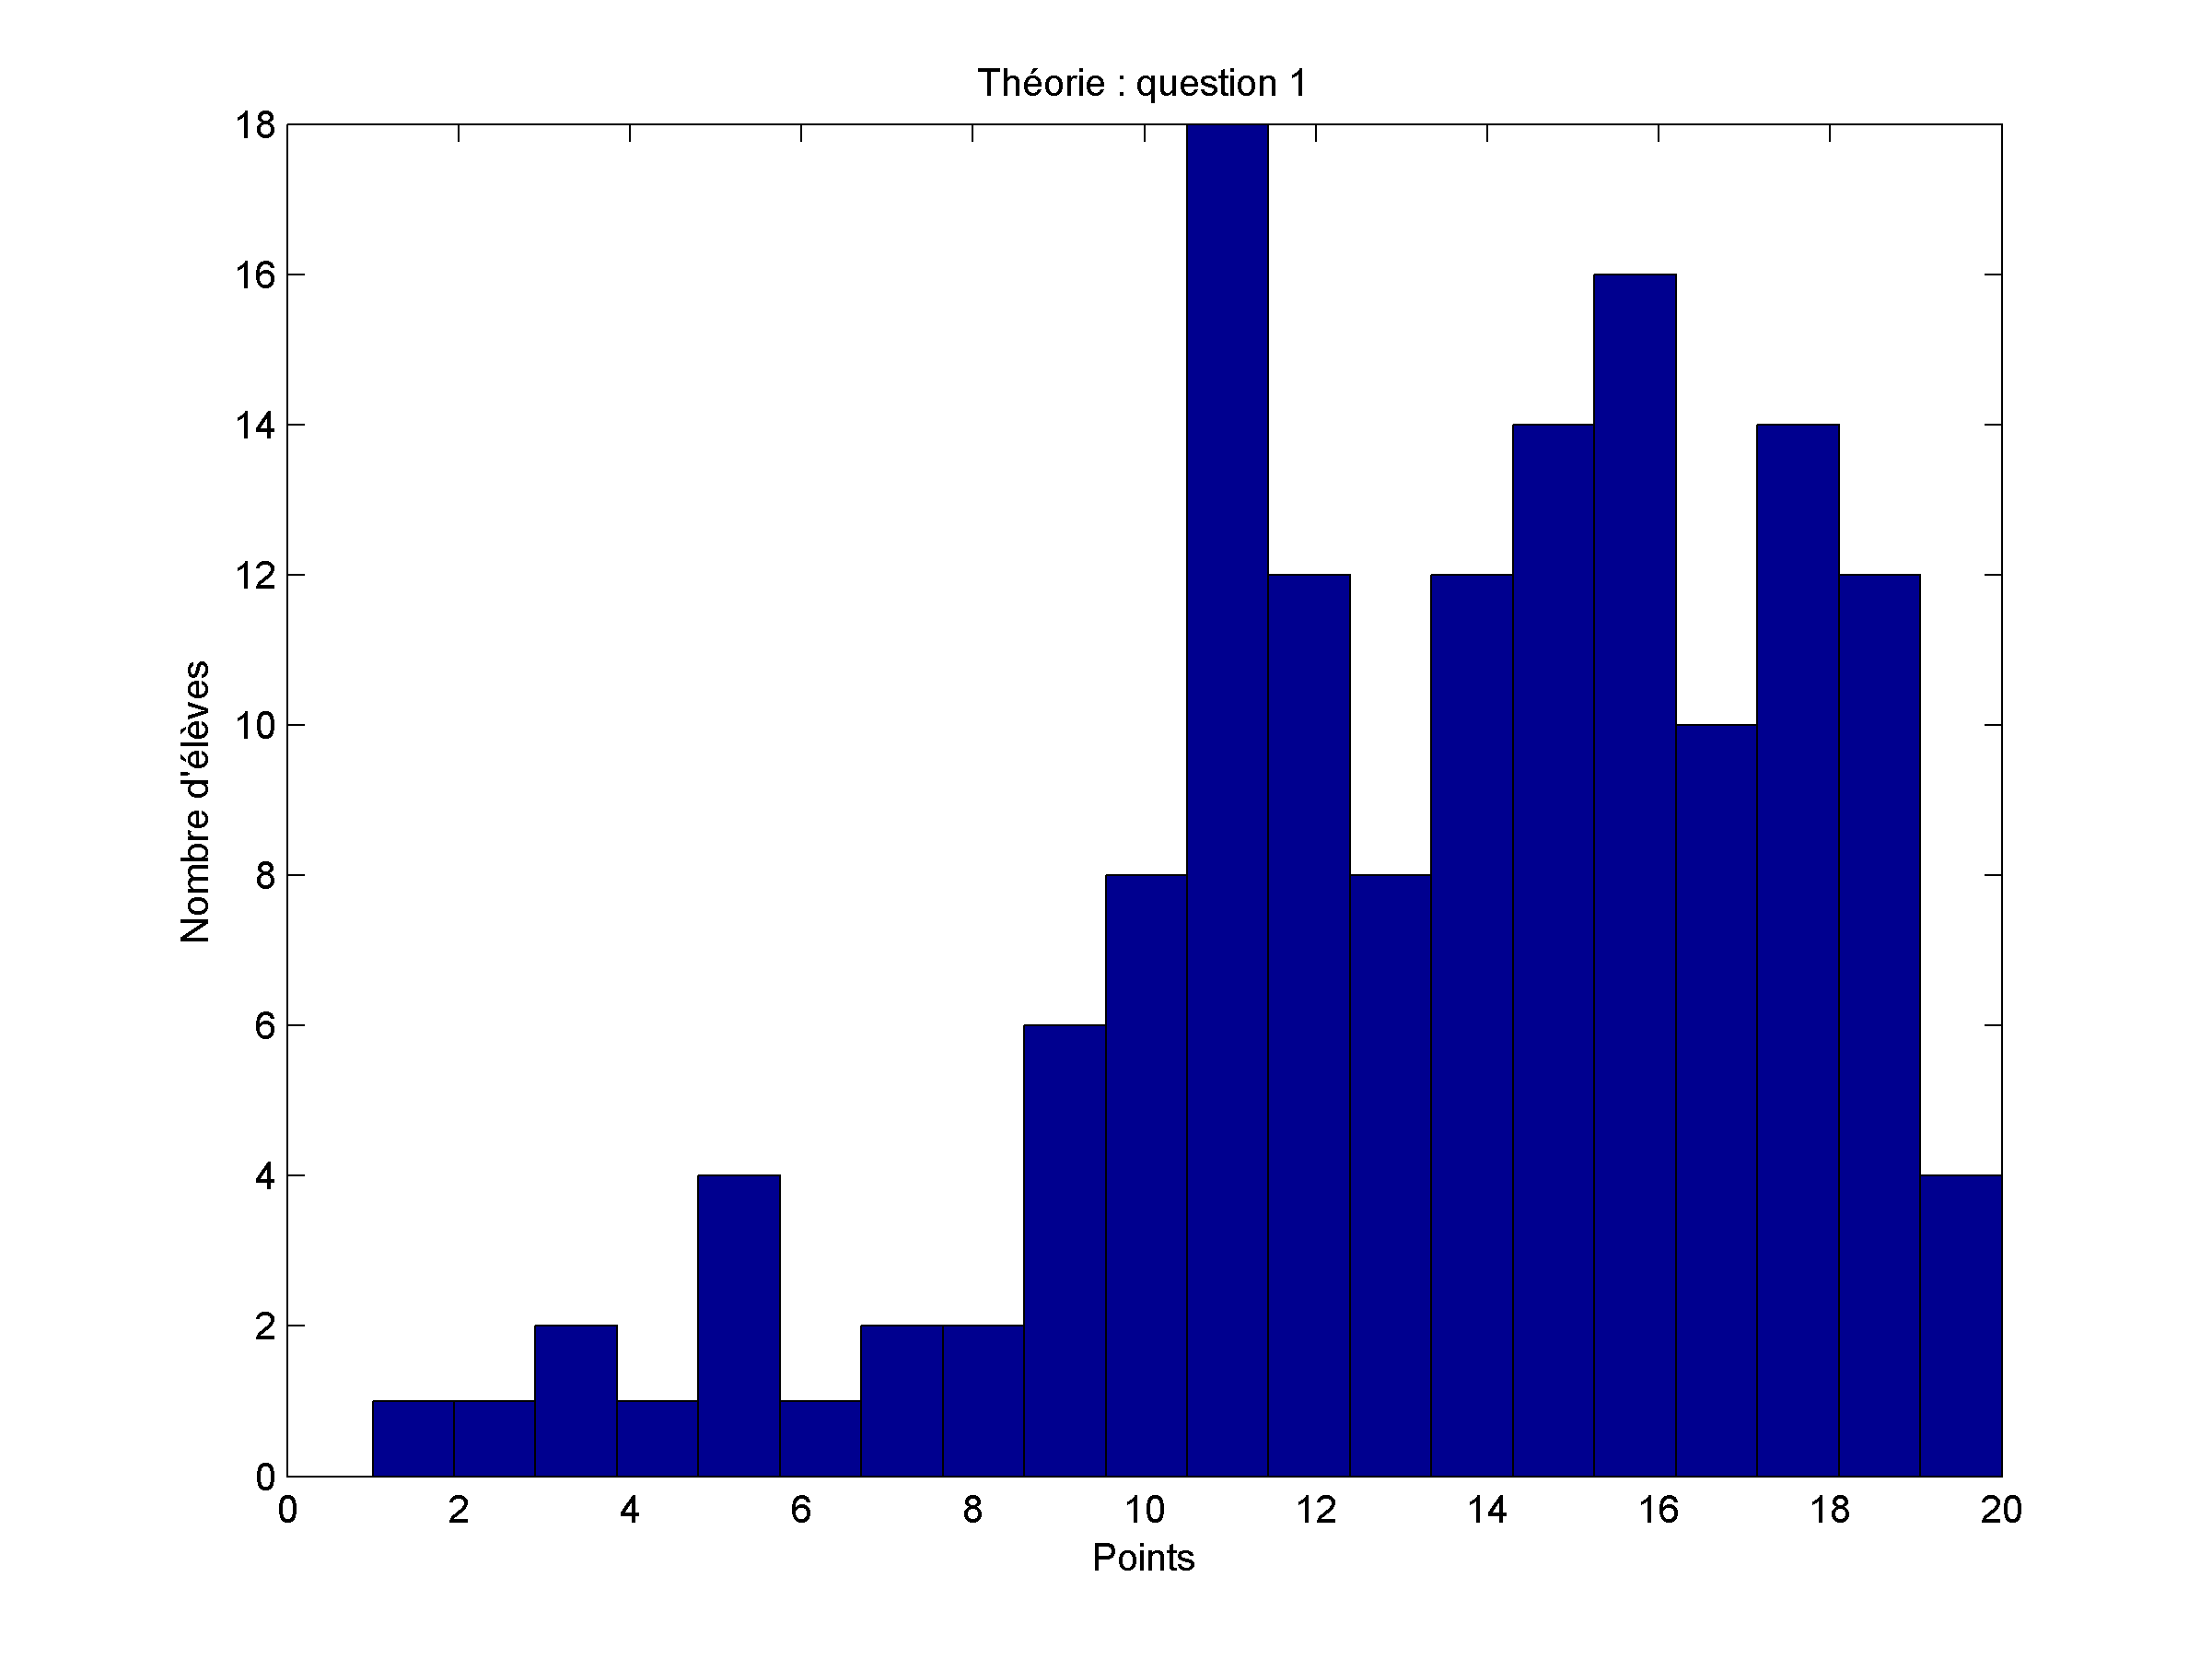
\includegraphics[scale=0.3]{q1a-hist-theo1.png}\label{fig:q1a_theo1}}
	\subfigure[Théorie 2]{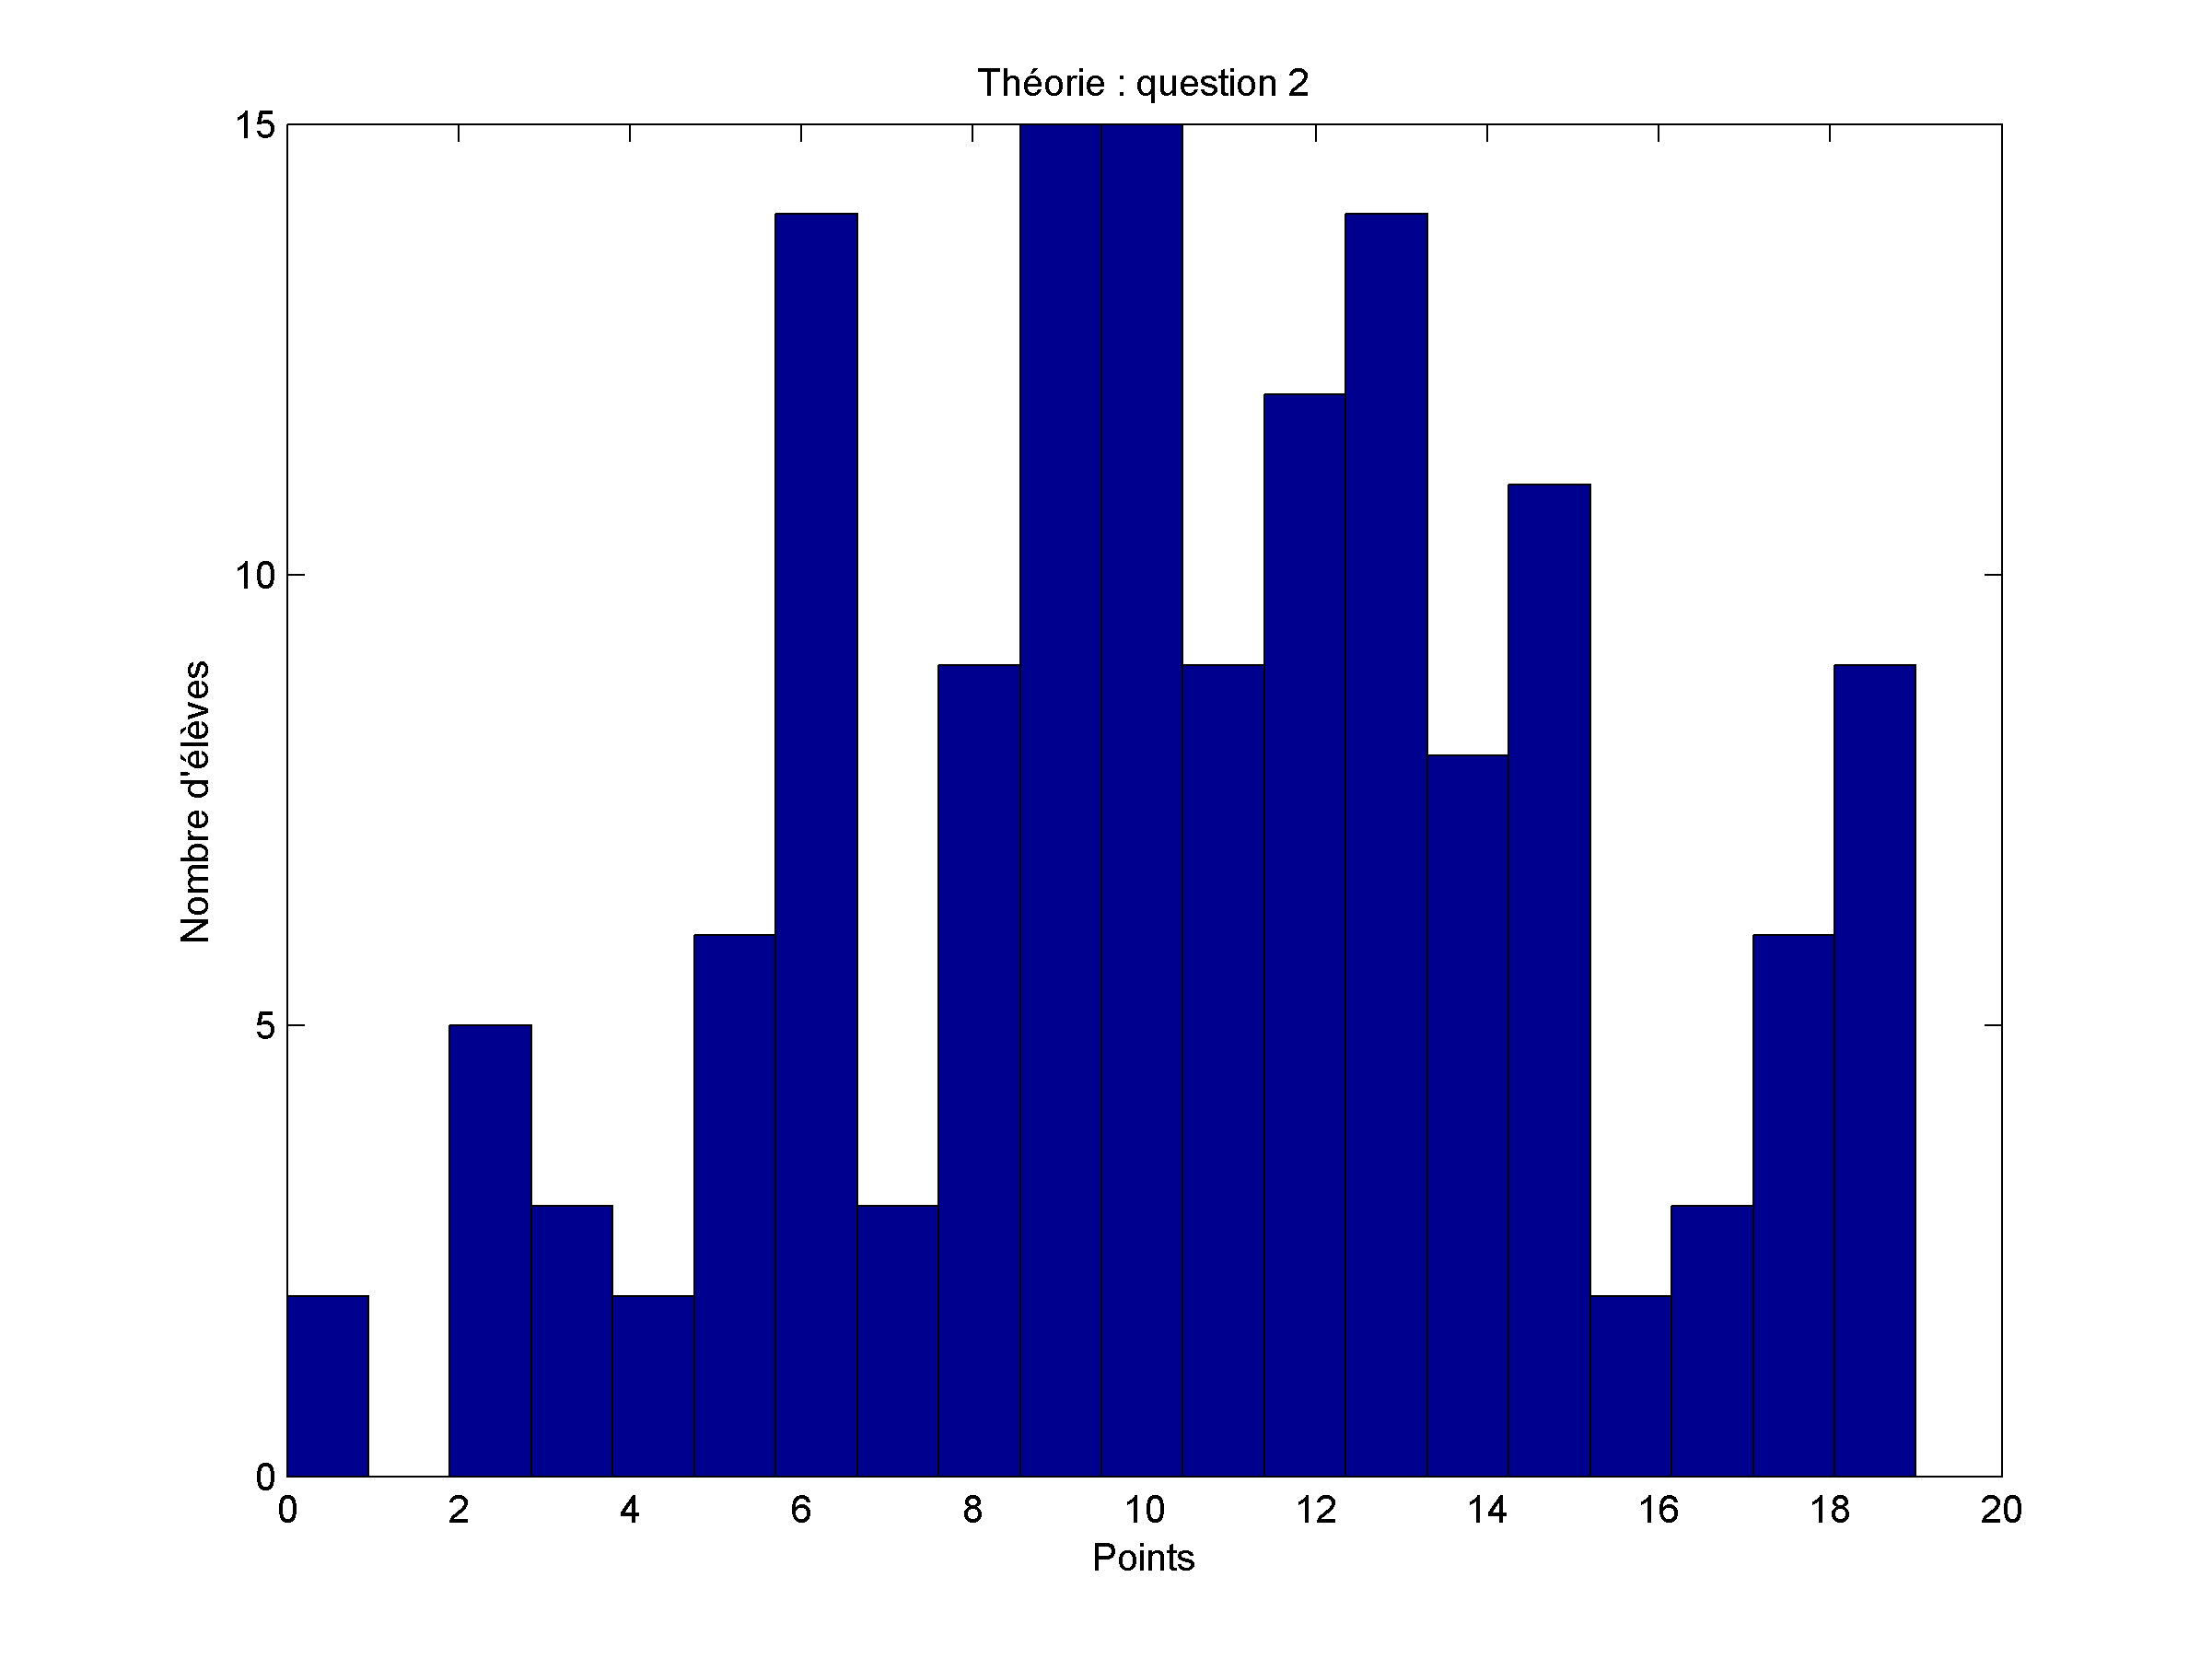
\includegraphics[scale=0.3]{q1a-hist-theo2.png}\label{fig:q1a_theo2}}
	\subfigure[Théorie 3]{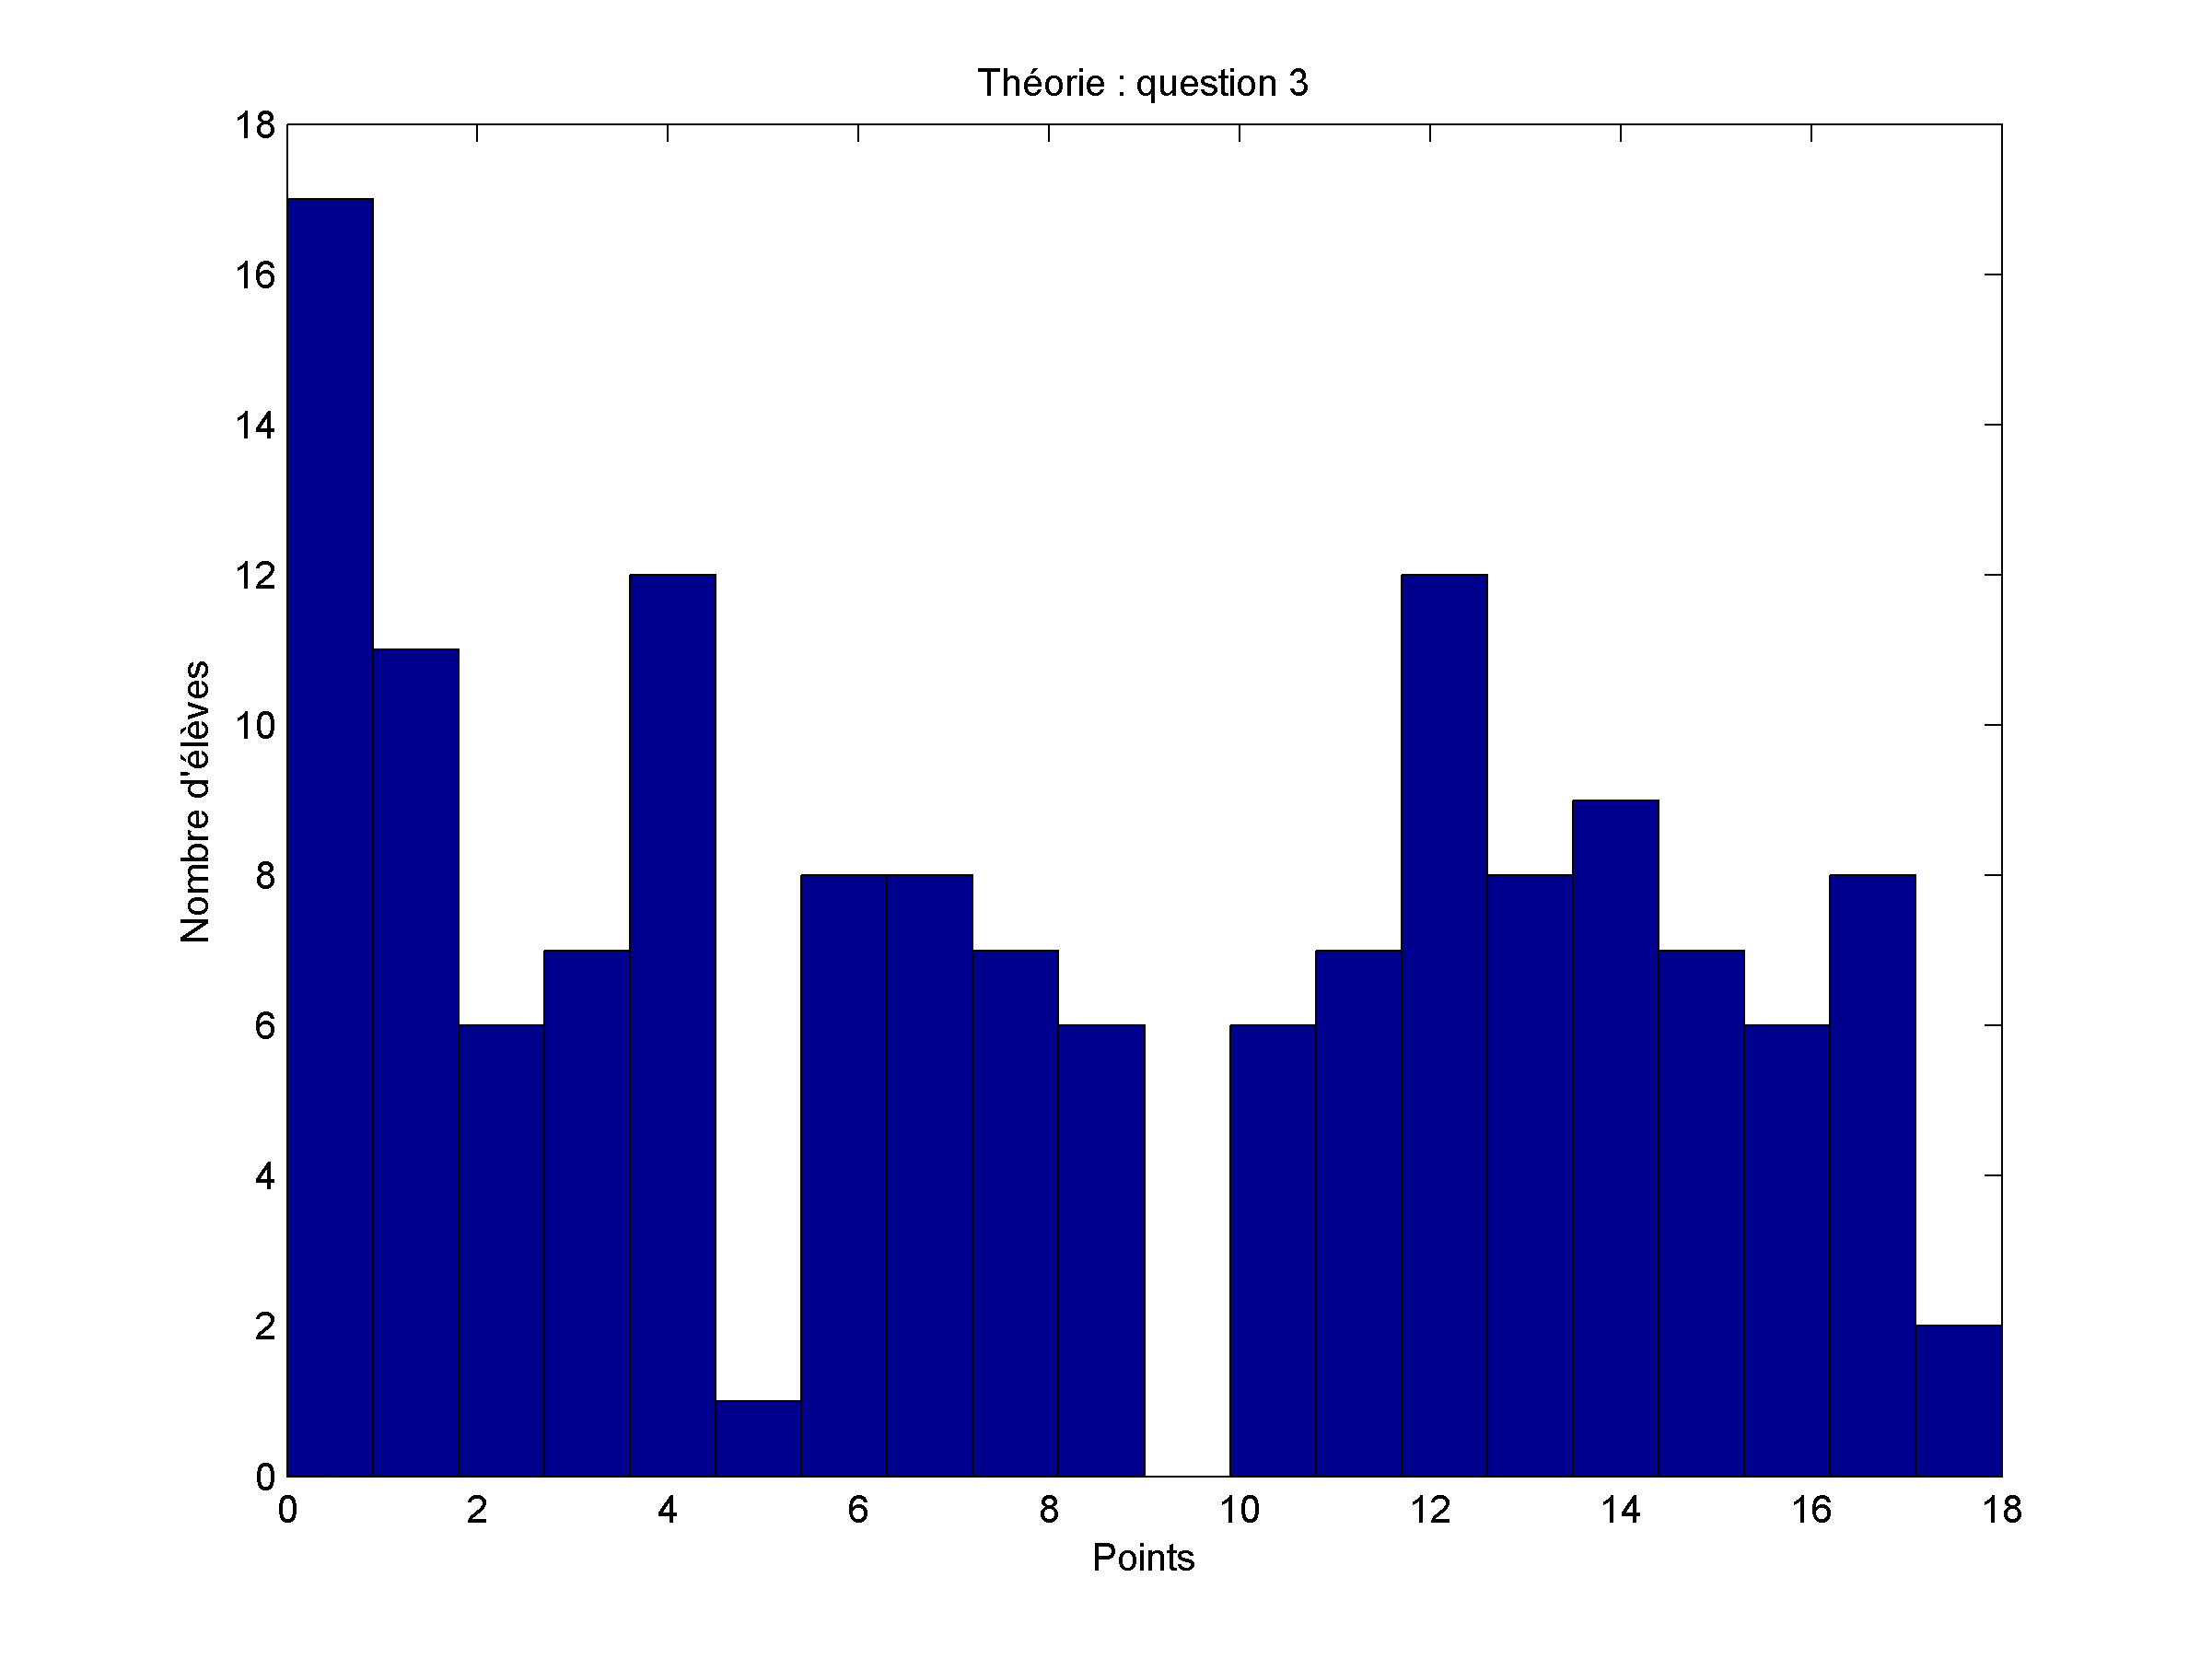
\includegraphics[scale=0.3]{q1a-hist-theo3.png}\label{fig:q1a_theo3}} 
	\caption{Fréquences pour les questions de théorie}
\end{figure}

\subsection{Point (b)} 
Les moyennes, modes, médianes et écarts types sont donnés dans la Table \ref{tab:exer_exam}. On constate que l'\textbf{exercice 2} a été \textbf{mieux réussi} que les deux autres. En effet, plus de la moitié des élèves ont eu 16 sur 20 ou plus et la cote la plus représentée est 20.
\paragraph{}
L'\textbf{exercice 3} a été quant à lui le \textbf{moins bien réussi} car plus de la moitié des élèves ont un moins de 5 sur 20 (ou 5 sur 20) avec une majorité d'élèves ayant eu 2.
\paragraph{}
En ce qui concerne les intervalles \textit{normaux} $[\mu_i - \sigma_i, \mu_i + \sigma_i]$, on trouve : 
\begin{itemize}
	\item pour la \textbf{question 1} : $64.86$\% des étudiants dans 	l'intervalle $[3.5549, 14.0937]$ (96 étudiants).
	\item pour la \textbf{question 2} : $57.43$\% des étudiants dans 	l'intervalle $[10.3998, 19.6948]$ (85 étudiants) 
	\item pour la \textbf{question 3} : $73.65$\% des étudiants dans 	l'intervalle $[1.4892, 9.6730]$ (109 étudiants)
\end{itemize} 

\begin{table}[h]
	\center
	\begin{tabular}{|c|c|c|c|c|}
		\hline
		Exercice & \textbf{Moyenne} & \textbf{Médiane} & \textbf{Mode} & \textbf{Écart-type}\\
		\hline
		\textbf{Question 1} & 8.8243 & 8 & 6 & 5.2694\\
		\textbf{Question 2} & 15.0473 & 16 & 20 & 4.6475\\
		\textbf{Question 3} & 5.5811 & 5 & 2 & 4.0919\\
		\hline
	\end{tabular}
	\caption{Exercices d'examen}
	\label{tab:exer_exam}
\end{table}

\subsection{Point (c)}
Les boîtes à moustaches mettent en évidence des résultats aberrants pour les trois projets mais pas pour la question d'examen sur le projet (voir Figure \ref{fig:q1c_boxplot}). Les valeurs aberrantes sont reprises dans la Table \ref{tab:q1c_aber}.
\paragraph{}
Les premier et troisième quartiles des résultats des projets et de la question d'examen sur le projet 3 sont donnés dans la Table \ref{tab:q1c_quart}.

\begin{figure}[h]
	\center
	\subfigure[Projet 1]{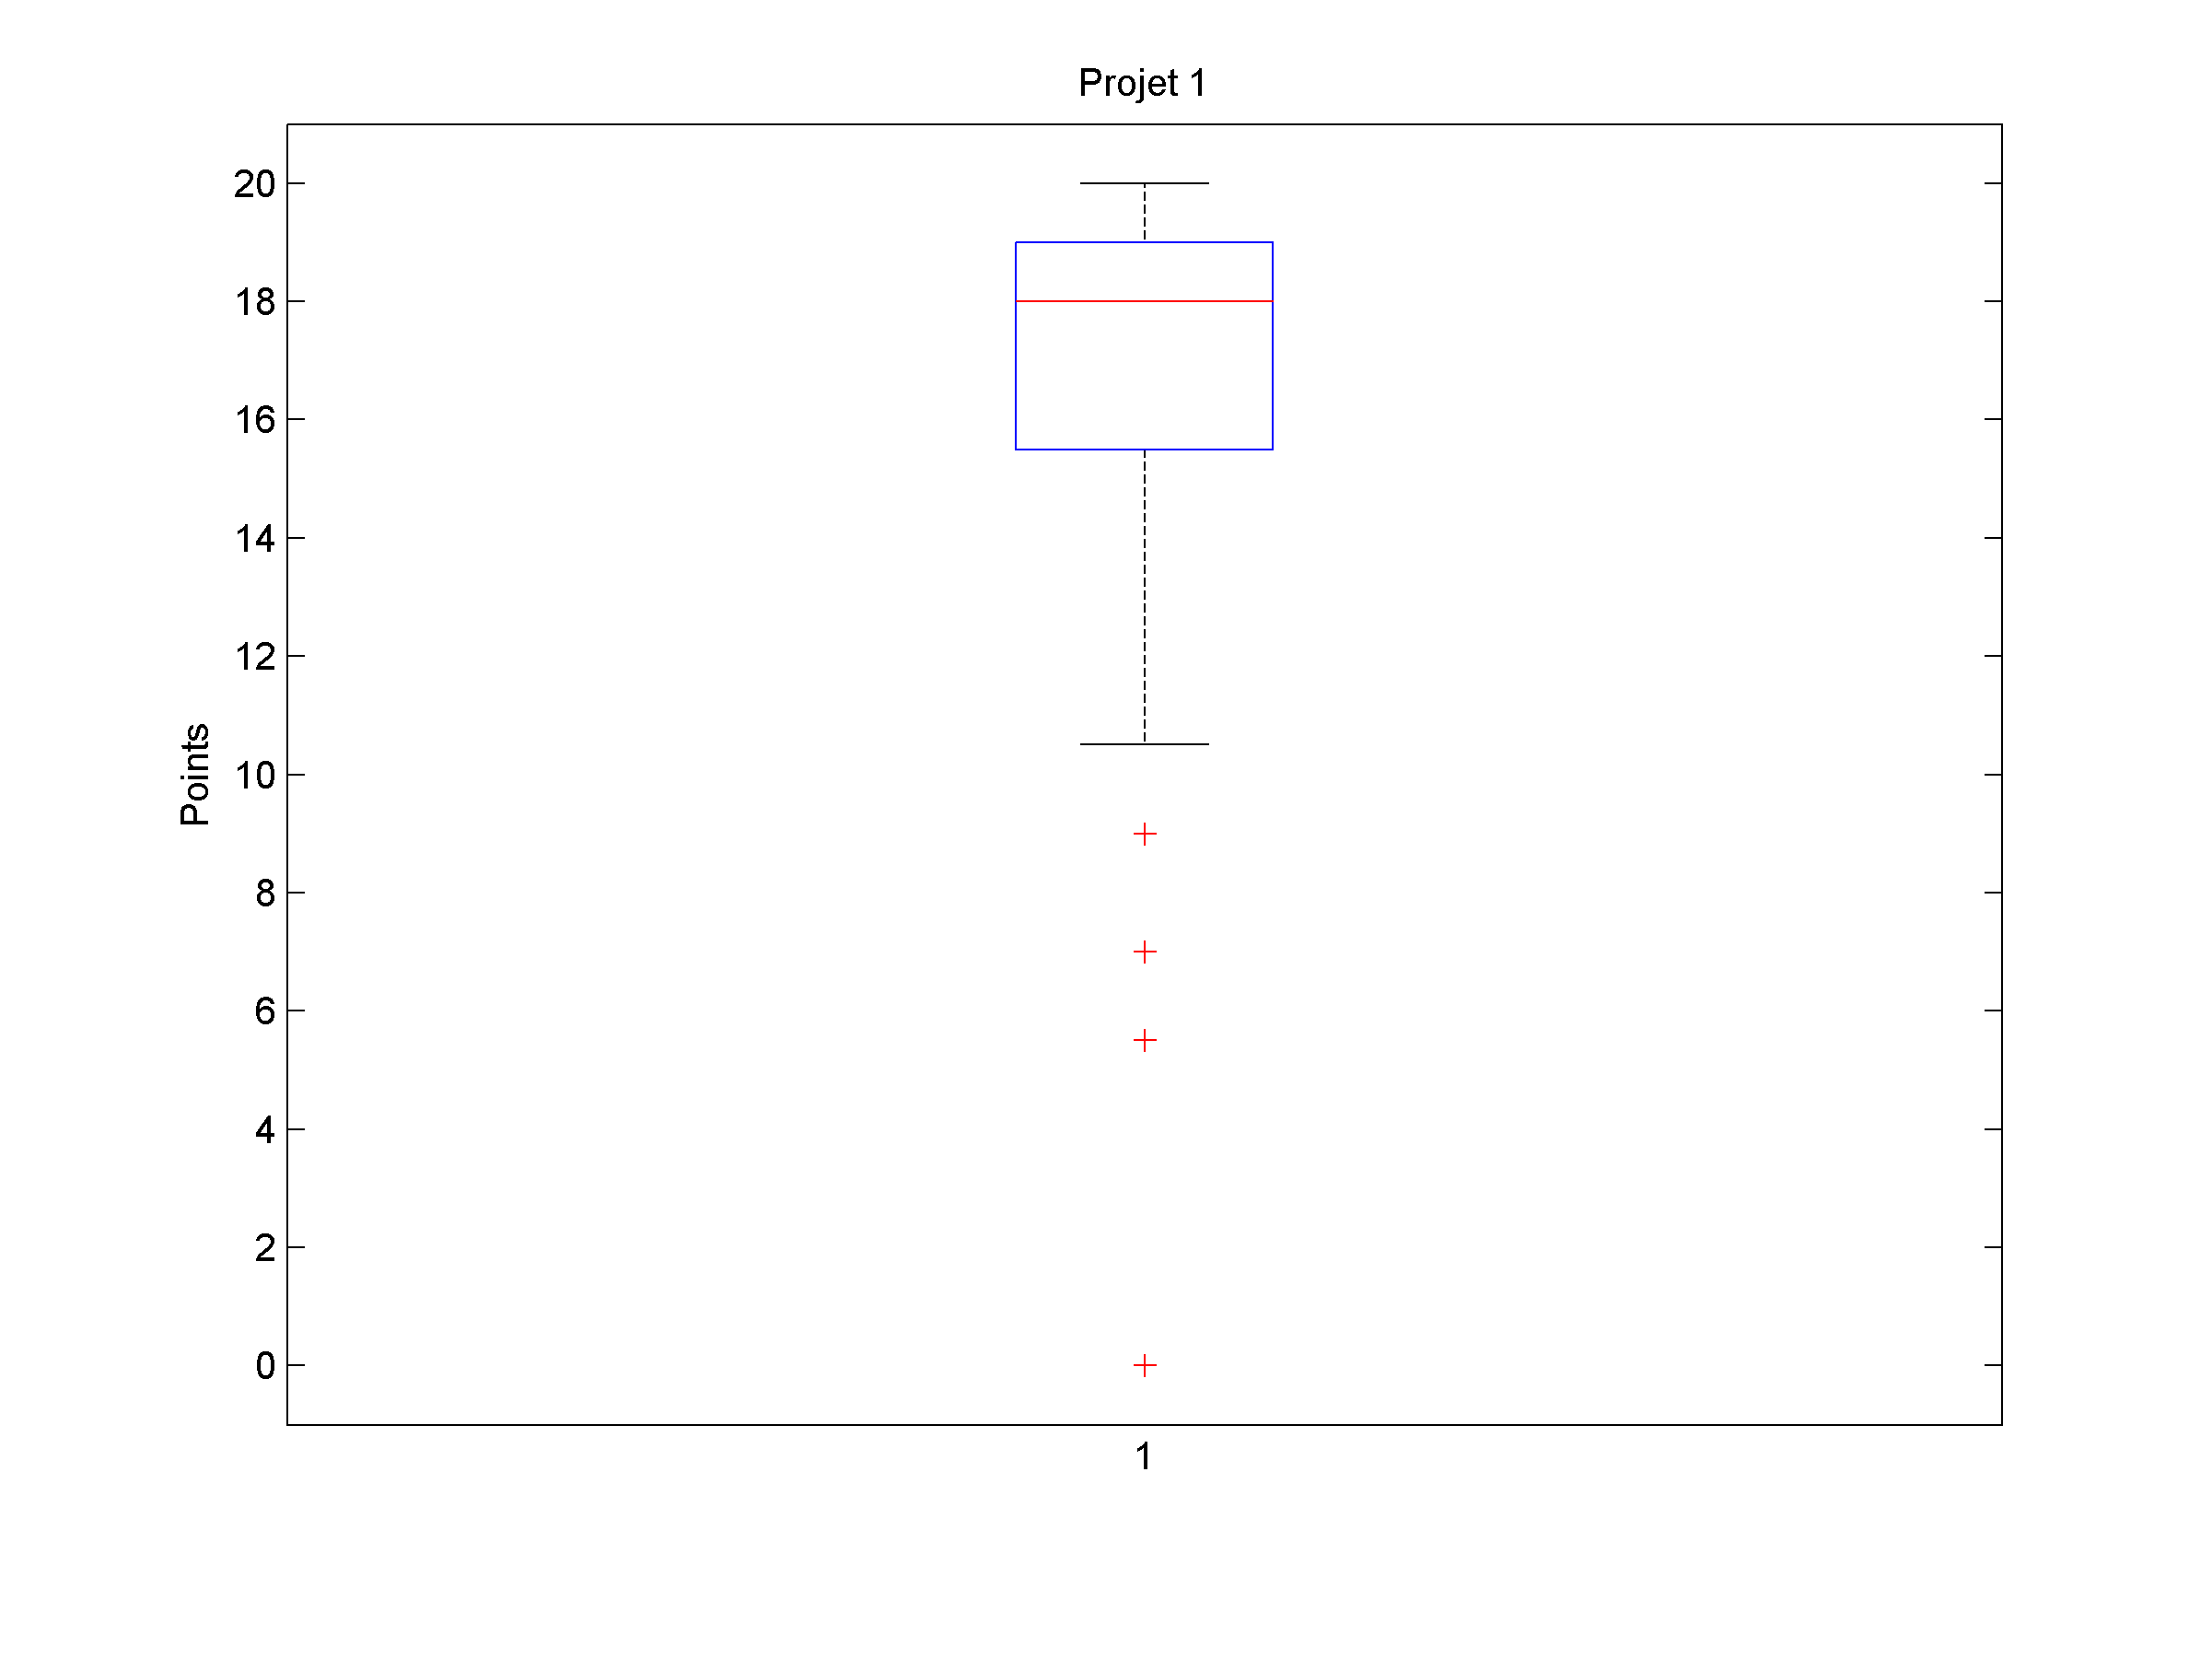
\includegraphics[scale=0.3]{q1cboxplotp1.png}}
	\subfigure[Projet 2]{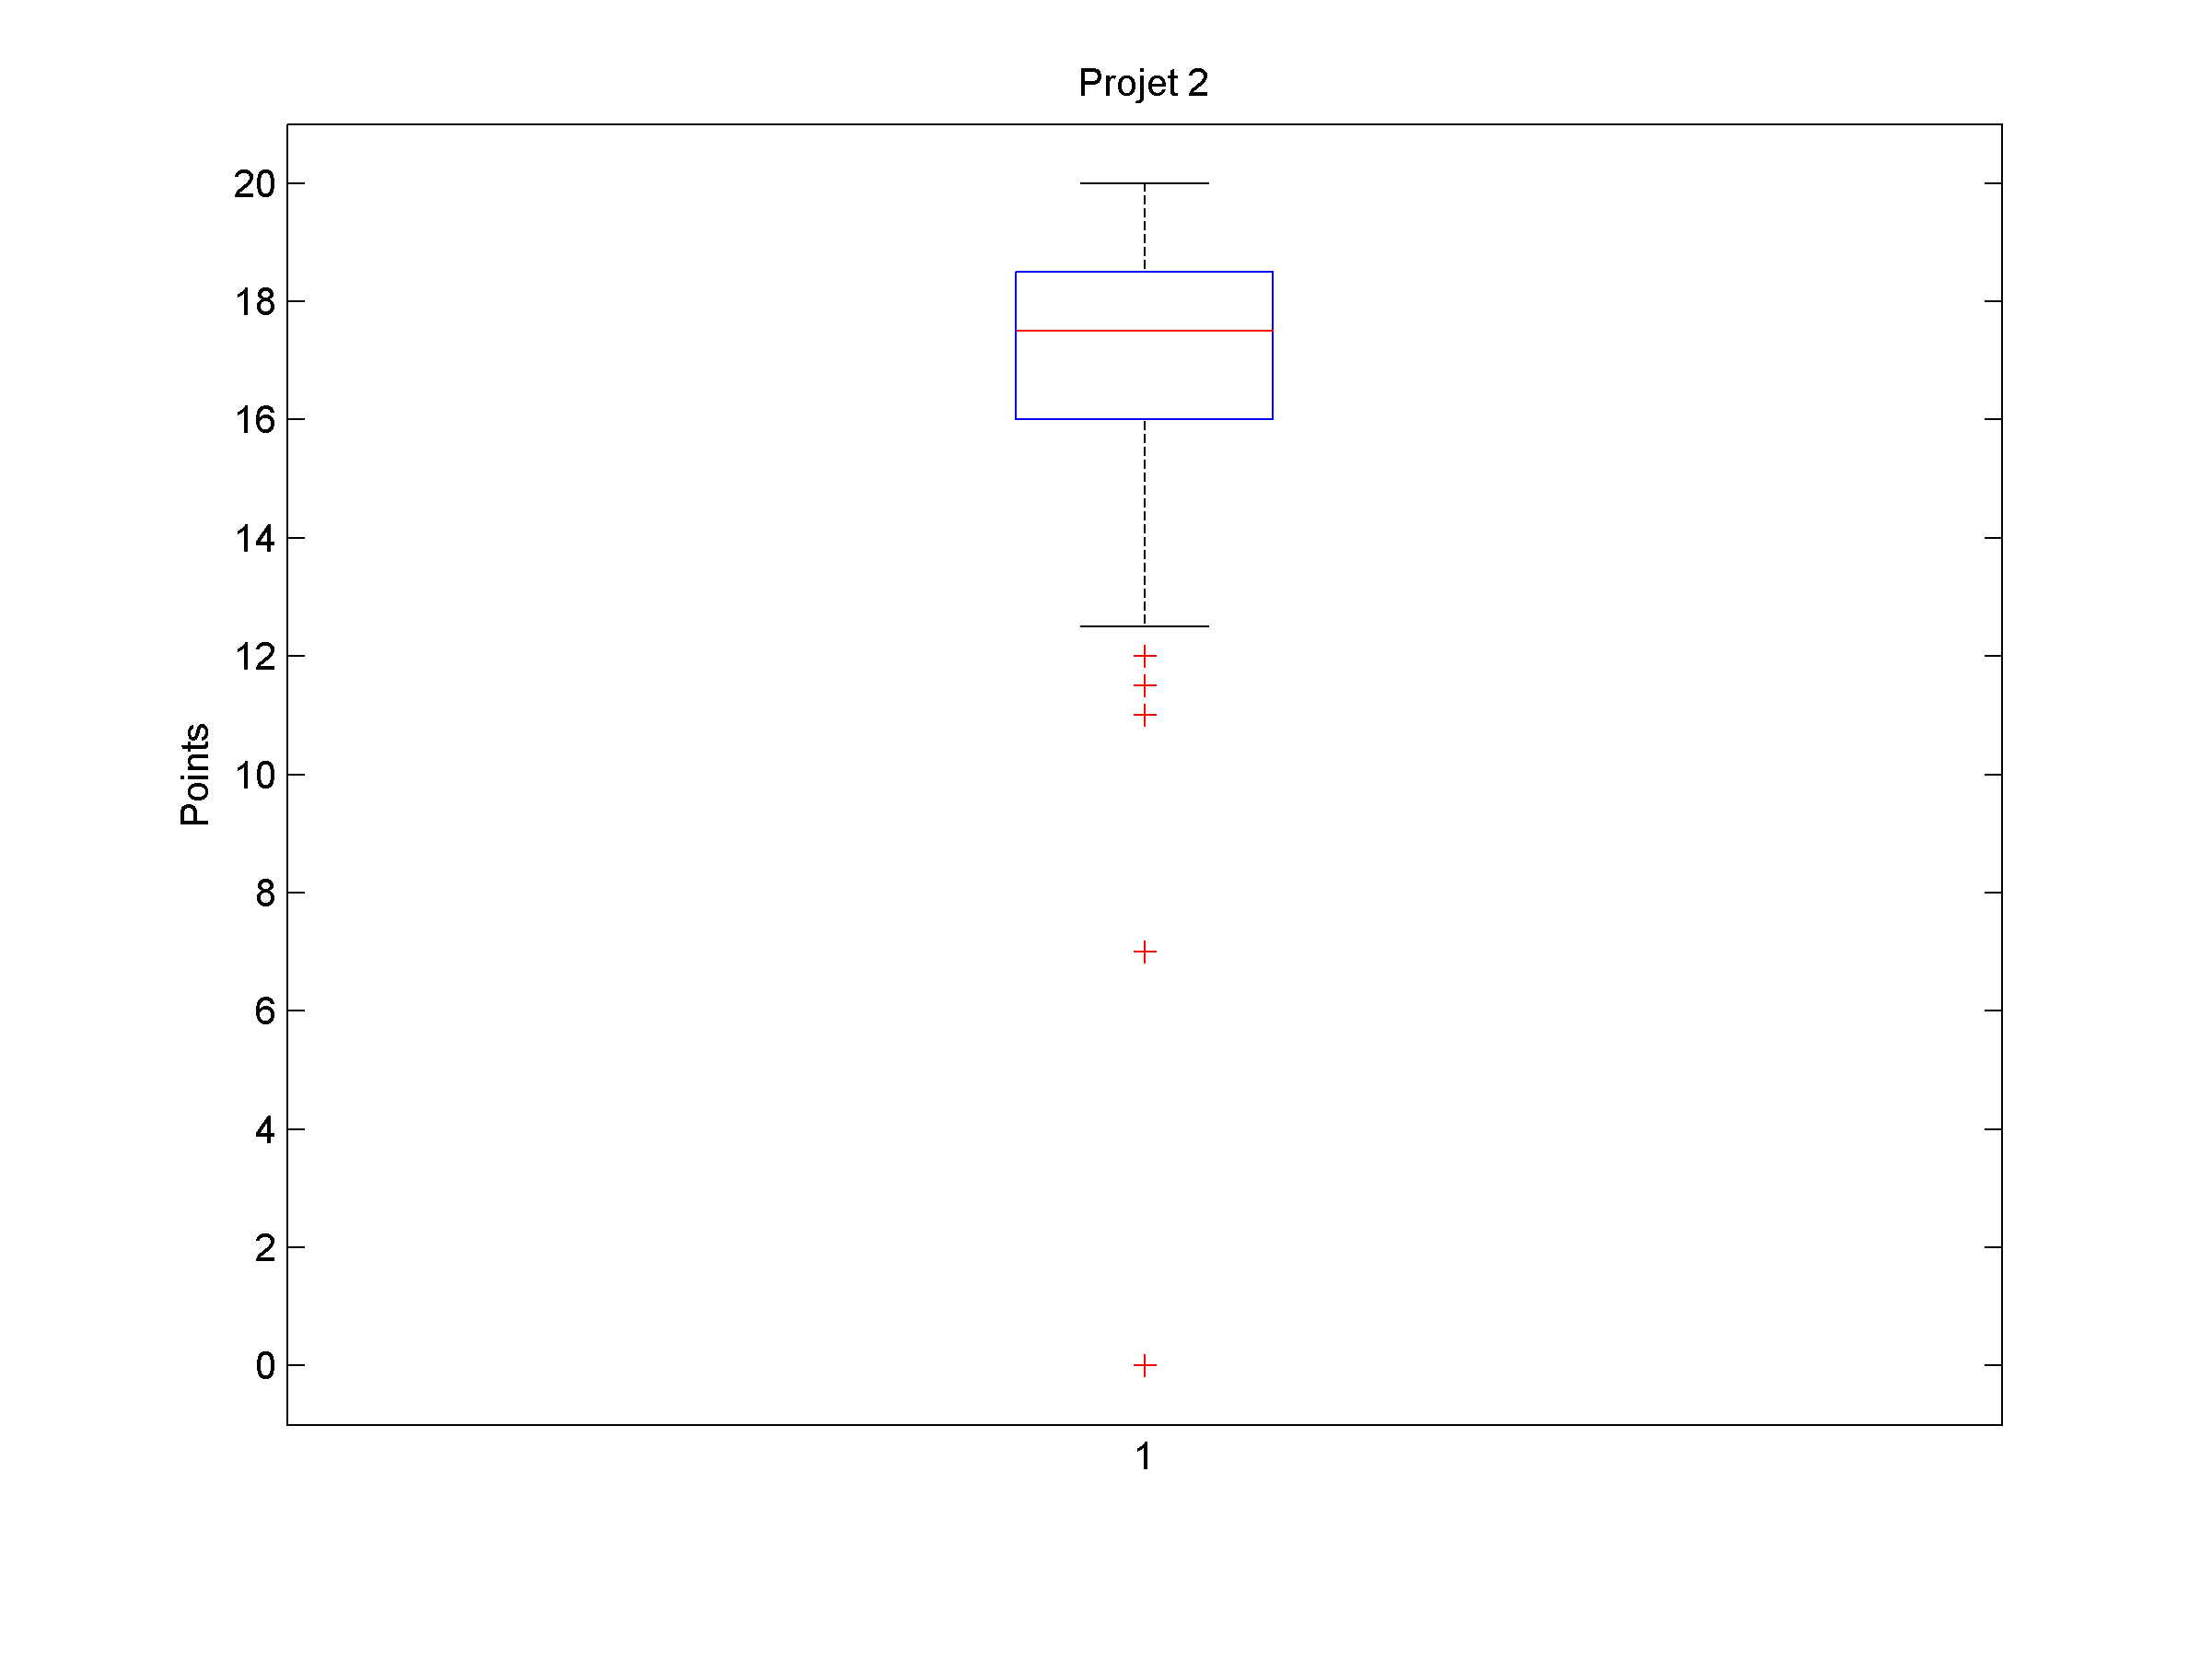
\includegraphics[scale=0.3]{q1cboxplotp2.png}}\\
	\subfigure[Projet 3]{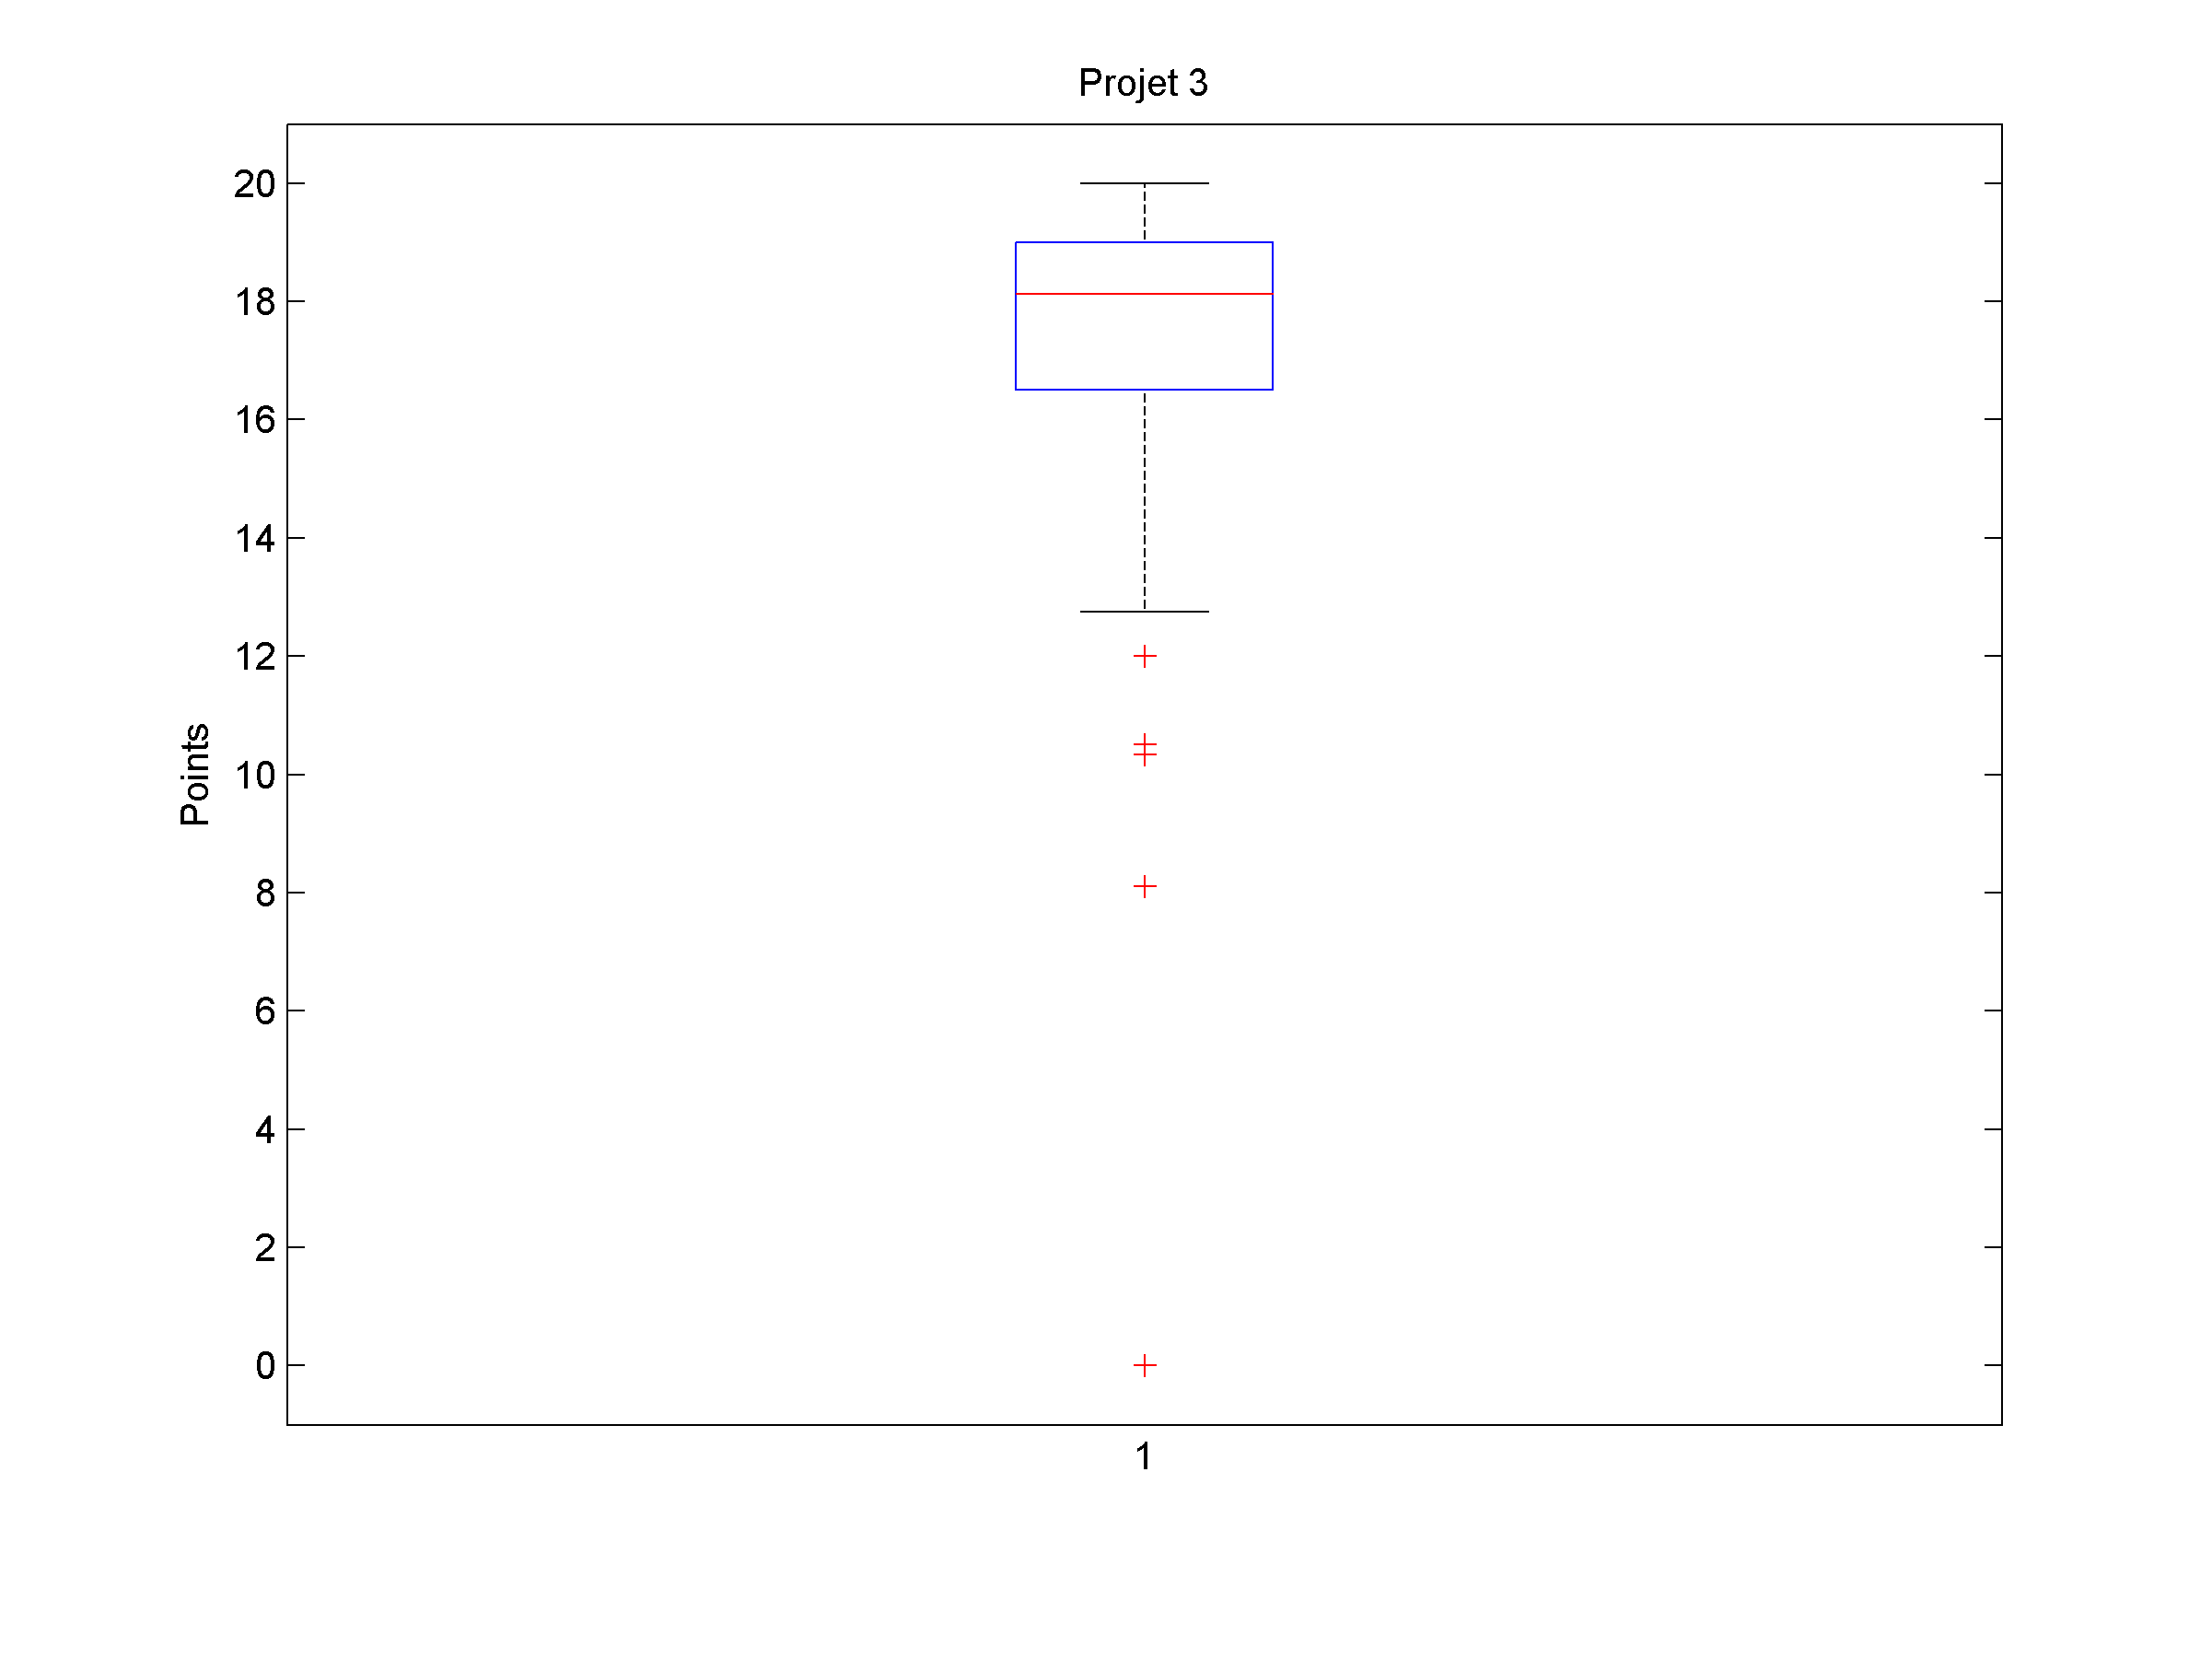
\includegraphics[scale=0.3]{q1cboxplotp3.png}}
	\subfigure[Examen : question sur le projet]{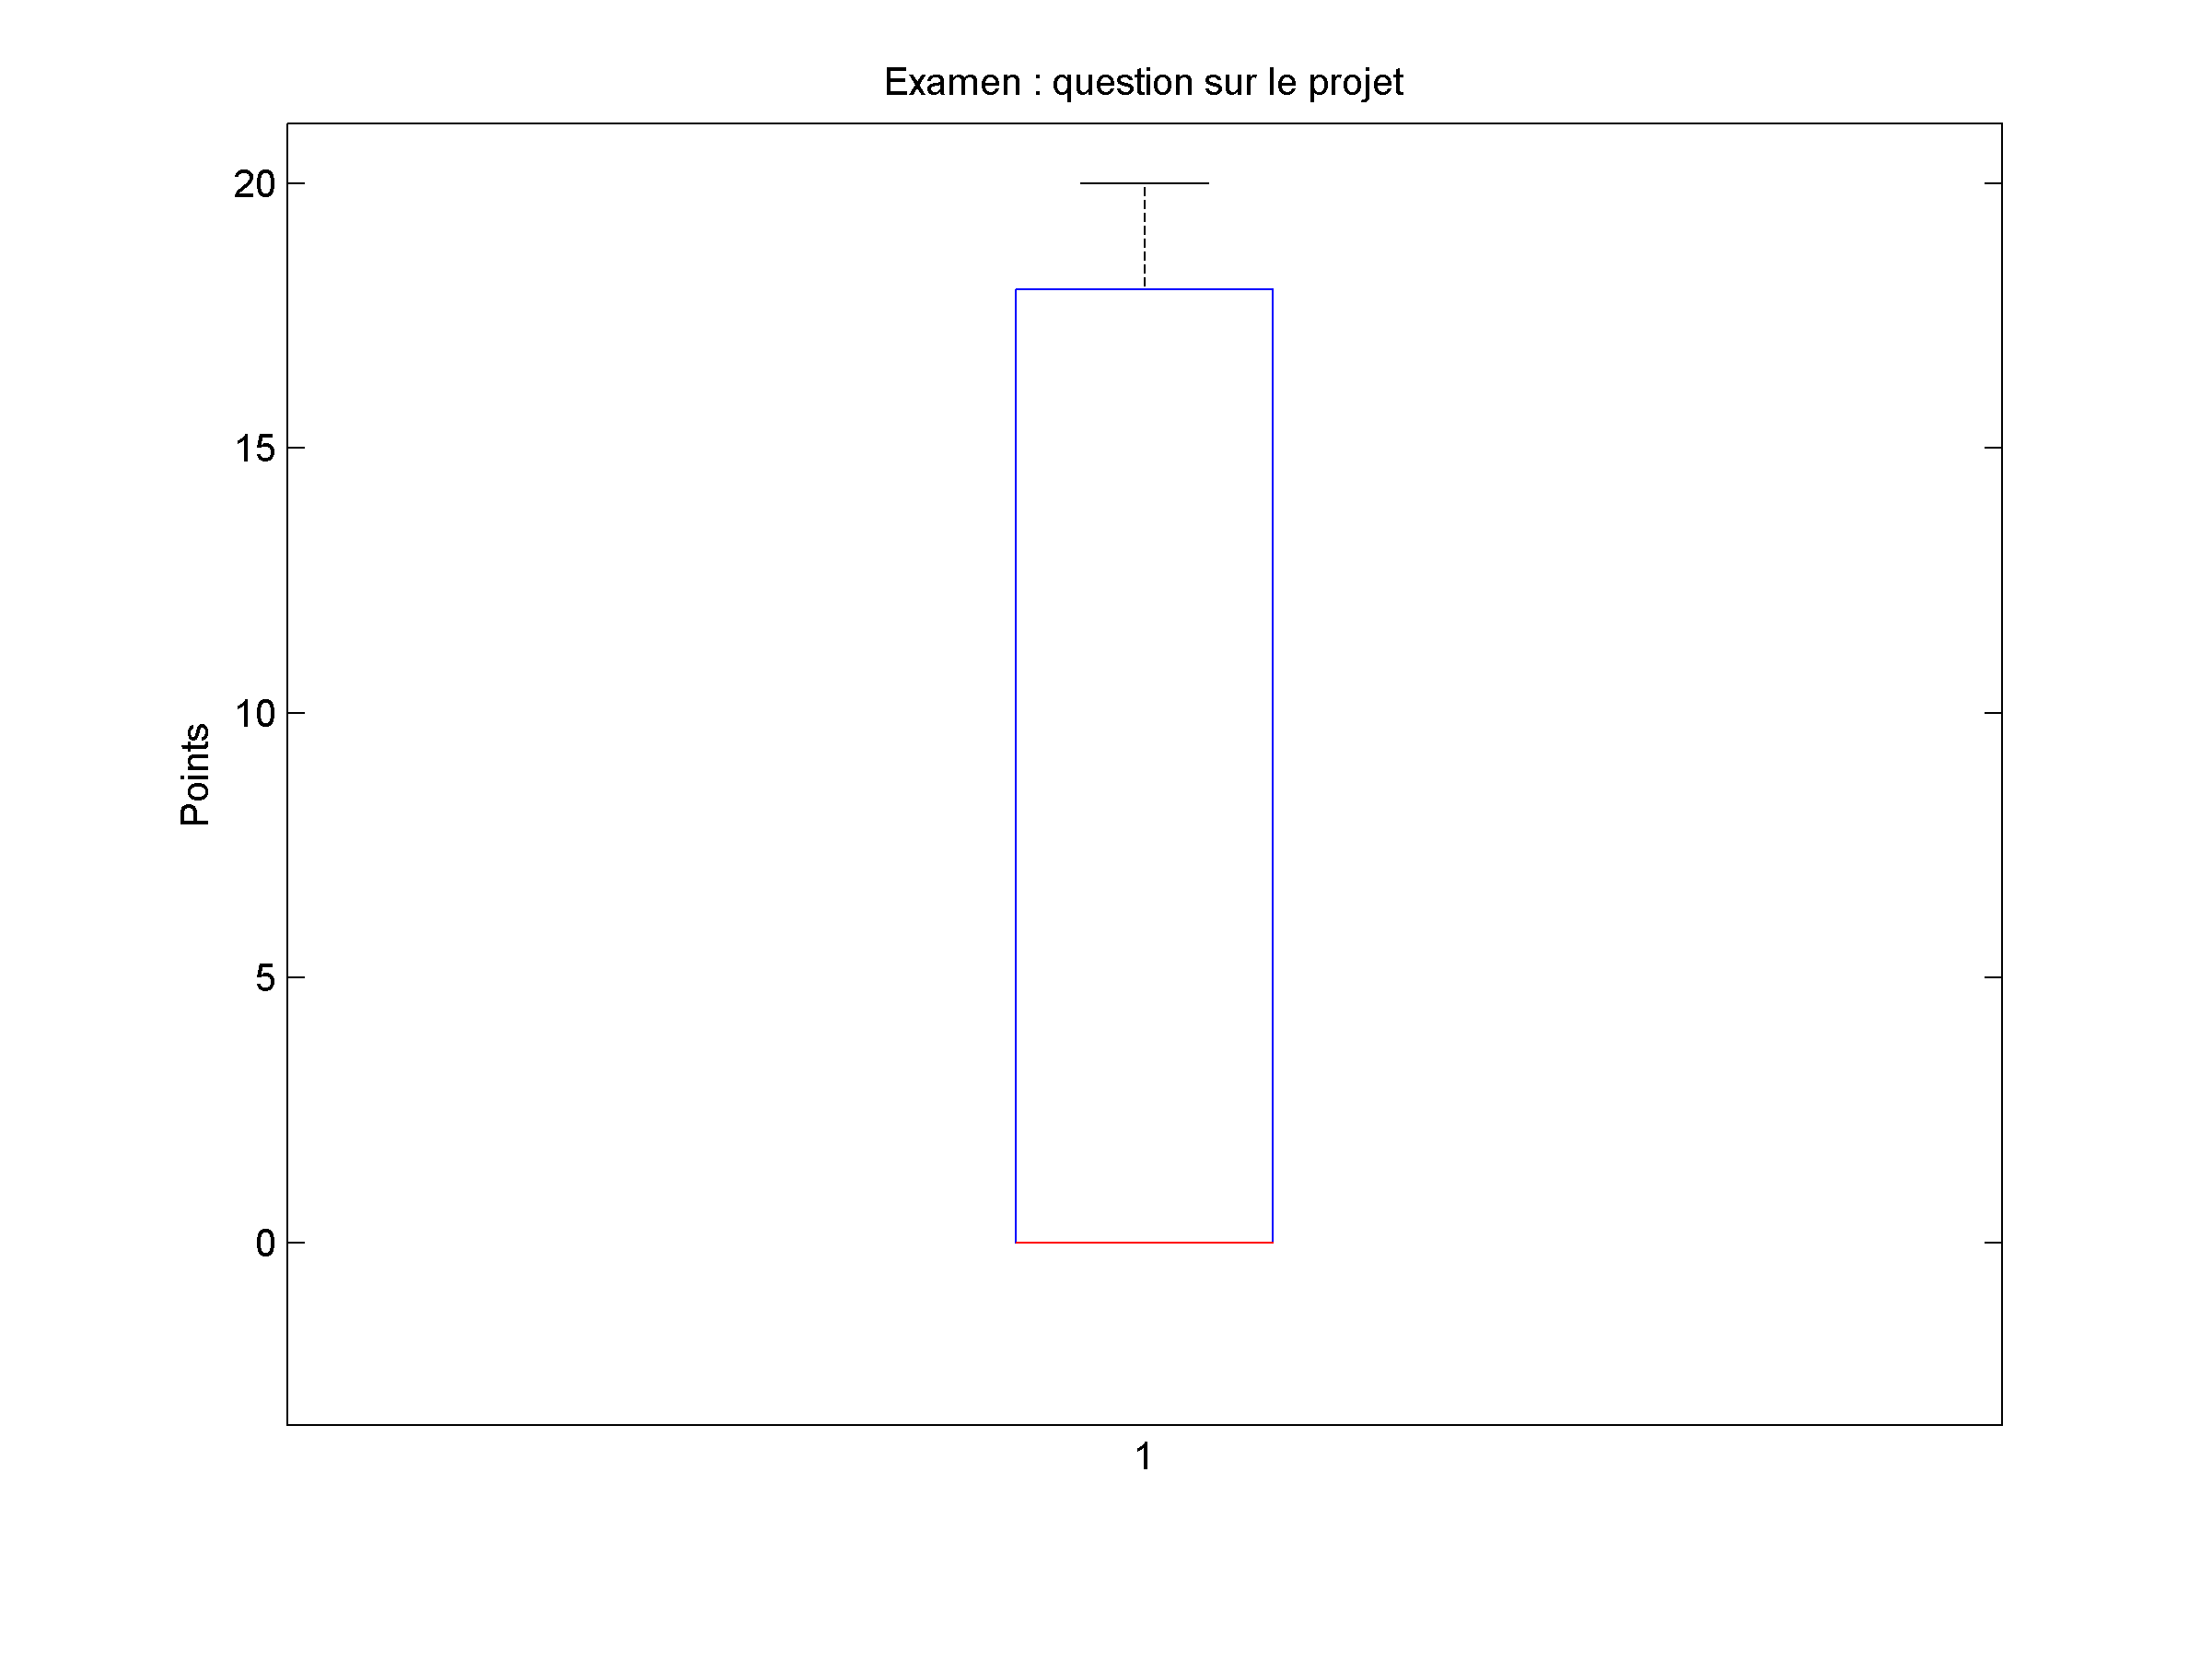
\includegraphics[scale=0.3]{q1cboxplotpe.png}}
	\caption{Résultat des projets et de la question sur le projet}
	\label{fig:q1c_boxplot}
\end{figure}


\begin{table}[h]
	\center
	\begin{tabular}{|c|c|}
		\hline
		\textbf{Projet} & \textbf{Notes aberrantes}\\
		\hline
		1 & 0 ($\times$ 4), 5.5, 7, 9\\
		2 & 0 ($\times$ 4), 7, 11, 11.5, 12\\
		3 & 0 ($\times$ 4), 8.11, 10.33, 10.5, 12 ($\times$ 3)\\
		\hline
	\end{tabular}
	\caption{Résultats aberrants pour les projets}
	\label{tab:q1c_aber}
\end{table}


\begin{table}[!h]
	\center
	\begin{tabular}{|c|cccc|}
	\hline
	Quartile & \textbf{Projet 1} & \textbf{Projet 2} & \textbf{Projet 3} & \textbf{Examen} \\
	\hline
	1$^{\text{er}}$ & 15.5 & 16 & 16.5 & 0\\
	3$^{\text{ème}}$ & 19 & 18.5 & 19 & 18\\
	\hline
	\end{tabular}
	\caption{Premier et troisième quartiles}
	\label{tab:q1c_quart}
\end{table}

\subsection{Point (d)}
Les graphiques des fréquences relatives cumulées pour les moyennes des questions de théorie et des questions d'exercice sont donnés respectivement sur les Figures \ref{fig:q1d_theo} et \ref{fig:q1d_exer}. La proportion d'étudiant ayant obtenu une cote dans un certain intervalle $[a,b]$ est obtenue à l'aide de la fonction des fréquences relatives cumulées $F$ :
\[
	F(a \leq x_i \leq b) = F(x_i = b) - F(x_i = a)  
\]
\paragraph{}
Les proportions obtenues pour l'intervalle $[12, 15]$ pour les moyennes théorie et l'exercice sont respectivement \textbf{18.24}\% et \textbf{22.30}\%. On constate, de plus, que la forme des graphes est similaire à la forme du graphe théorique de la fréquence relative cumulée pour une loi normale (surtout pour la moyenne de théorie).

\begin{figure}
	\subfigure[Théorie]{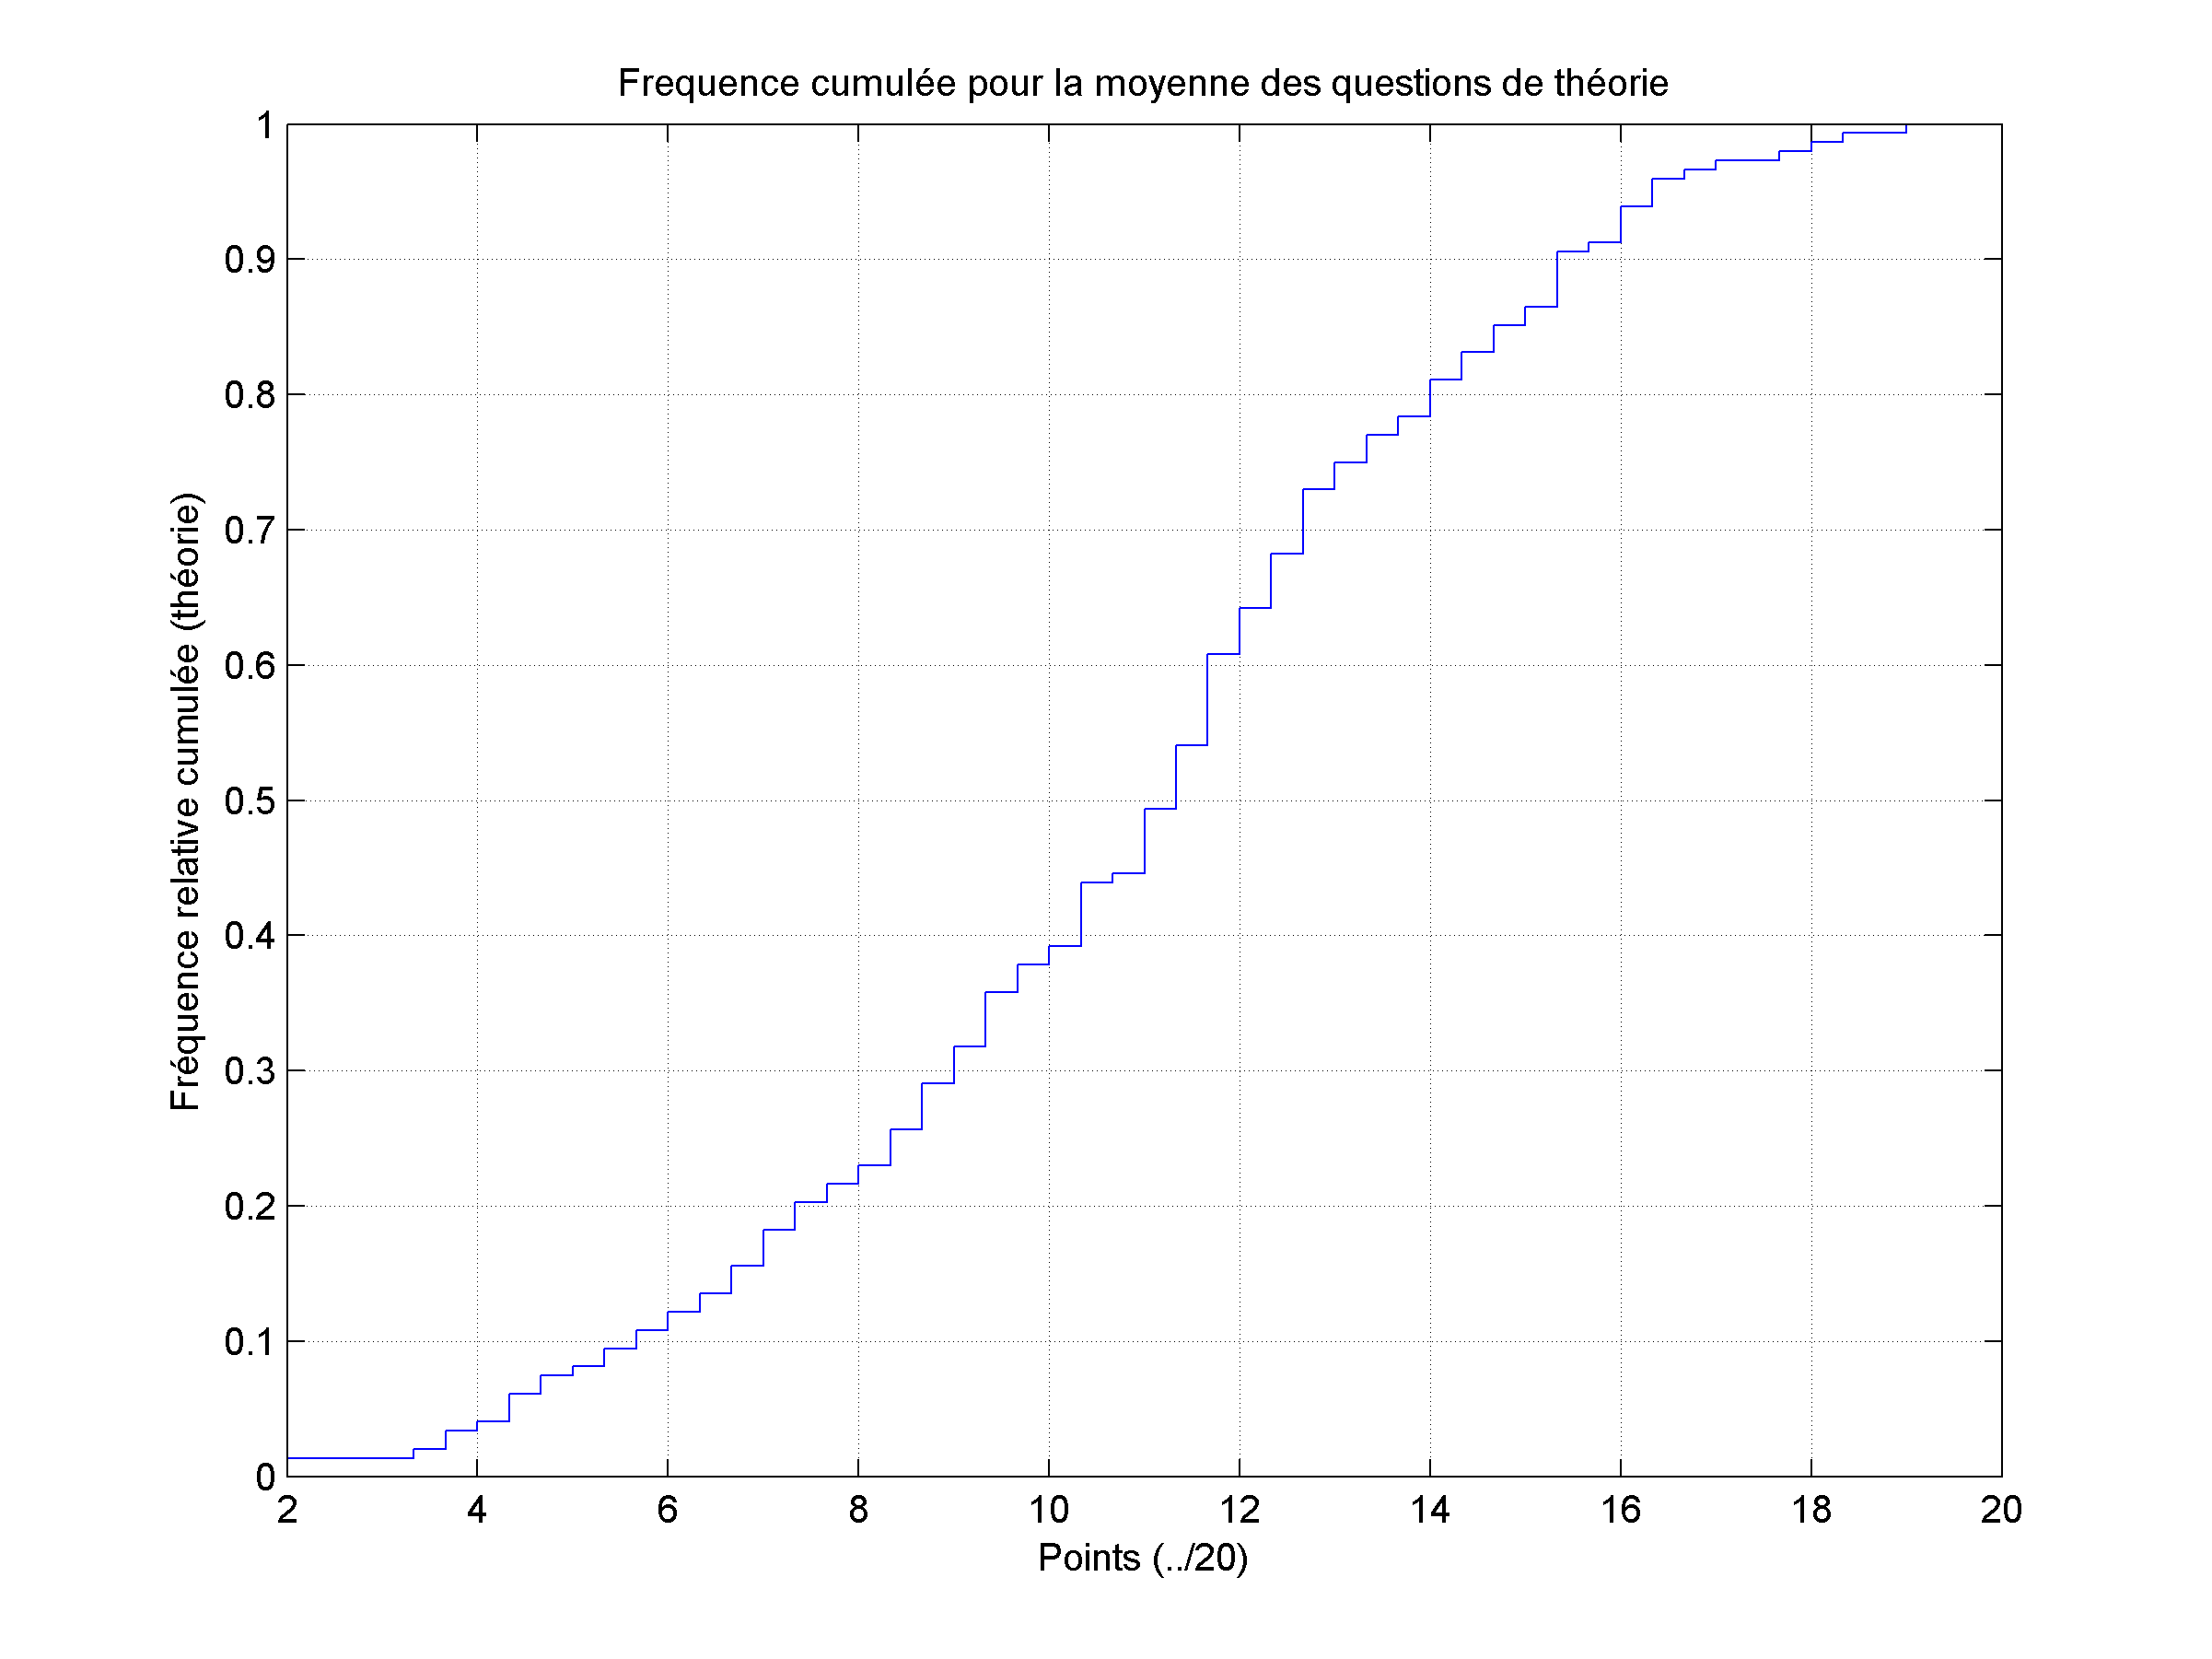
\includegraphics[scale=0.4]{q1d-cdfplot-theo.png}\label{fig:q1d_theo}}
	\subfigure[Exercice]{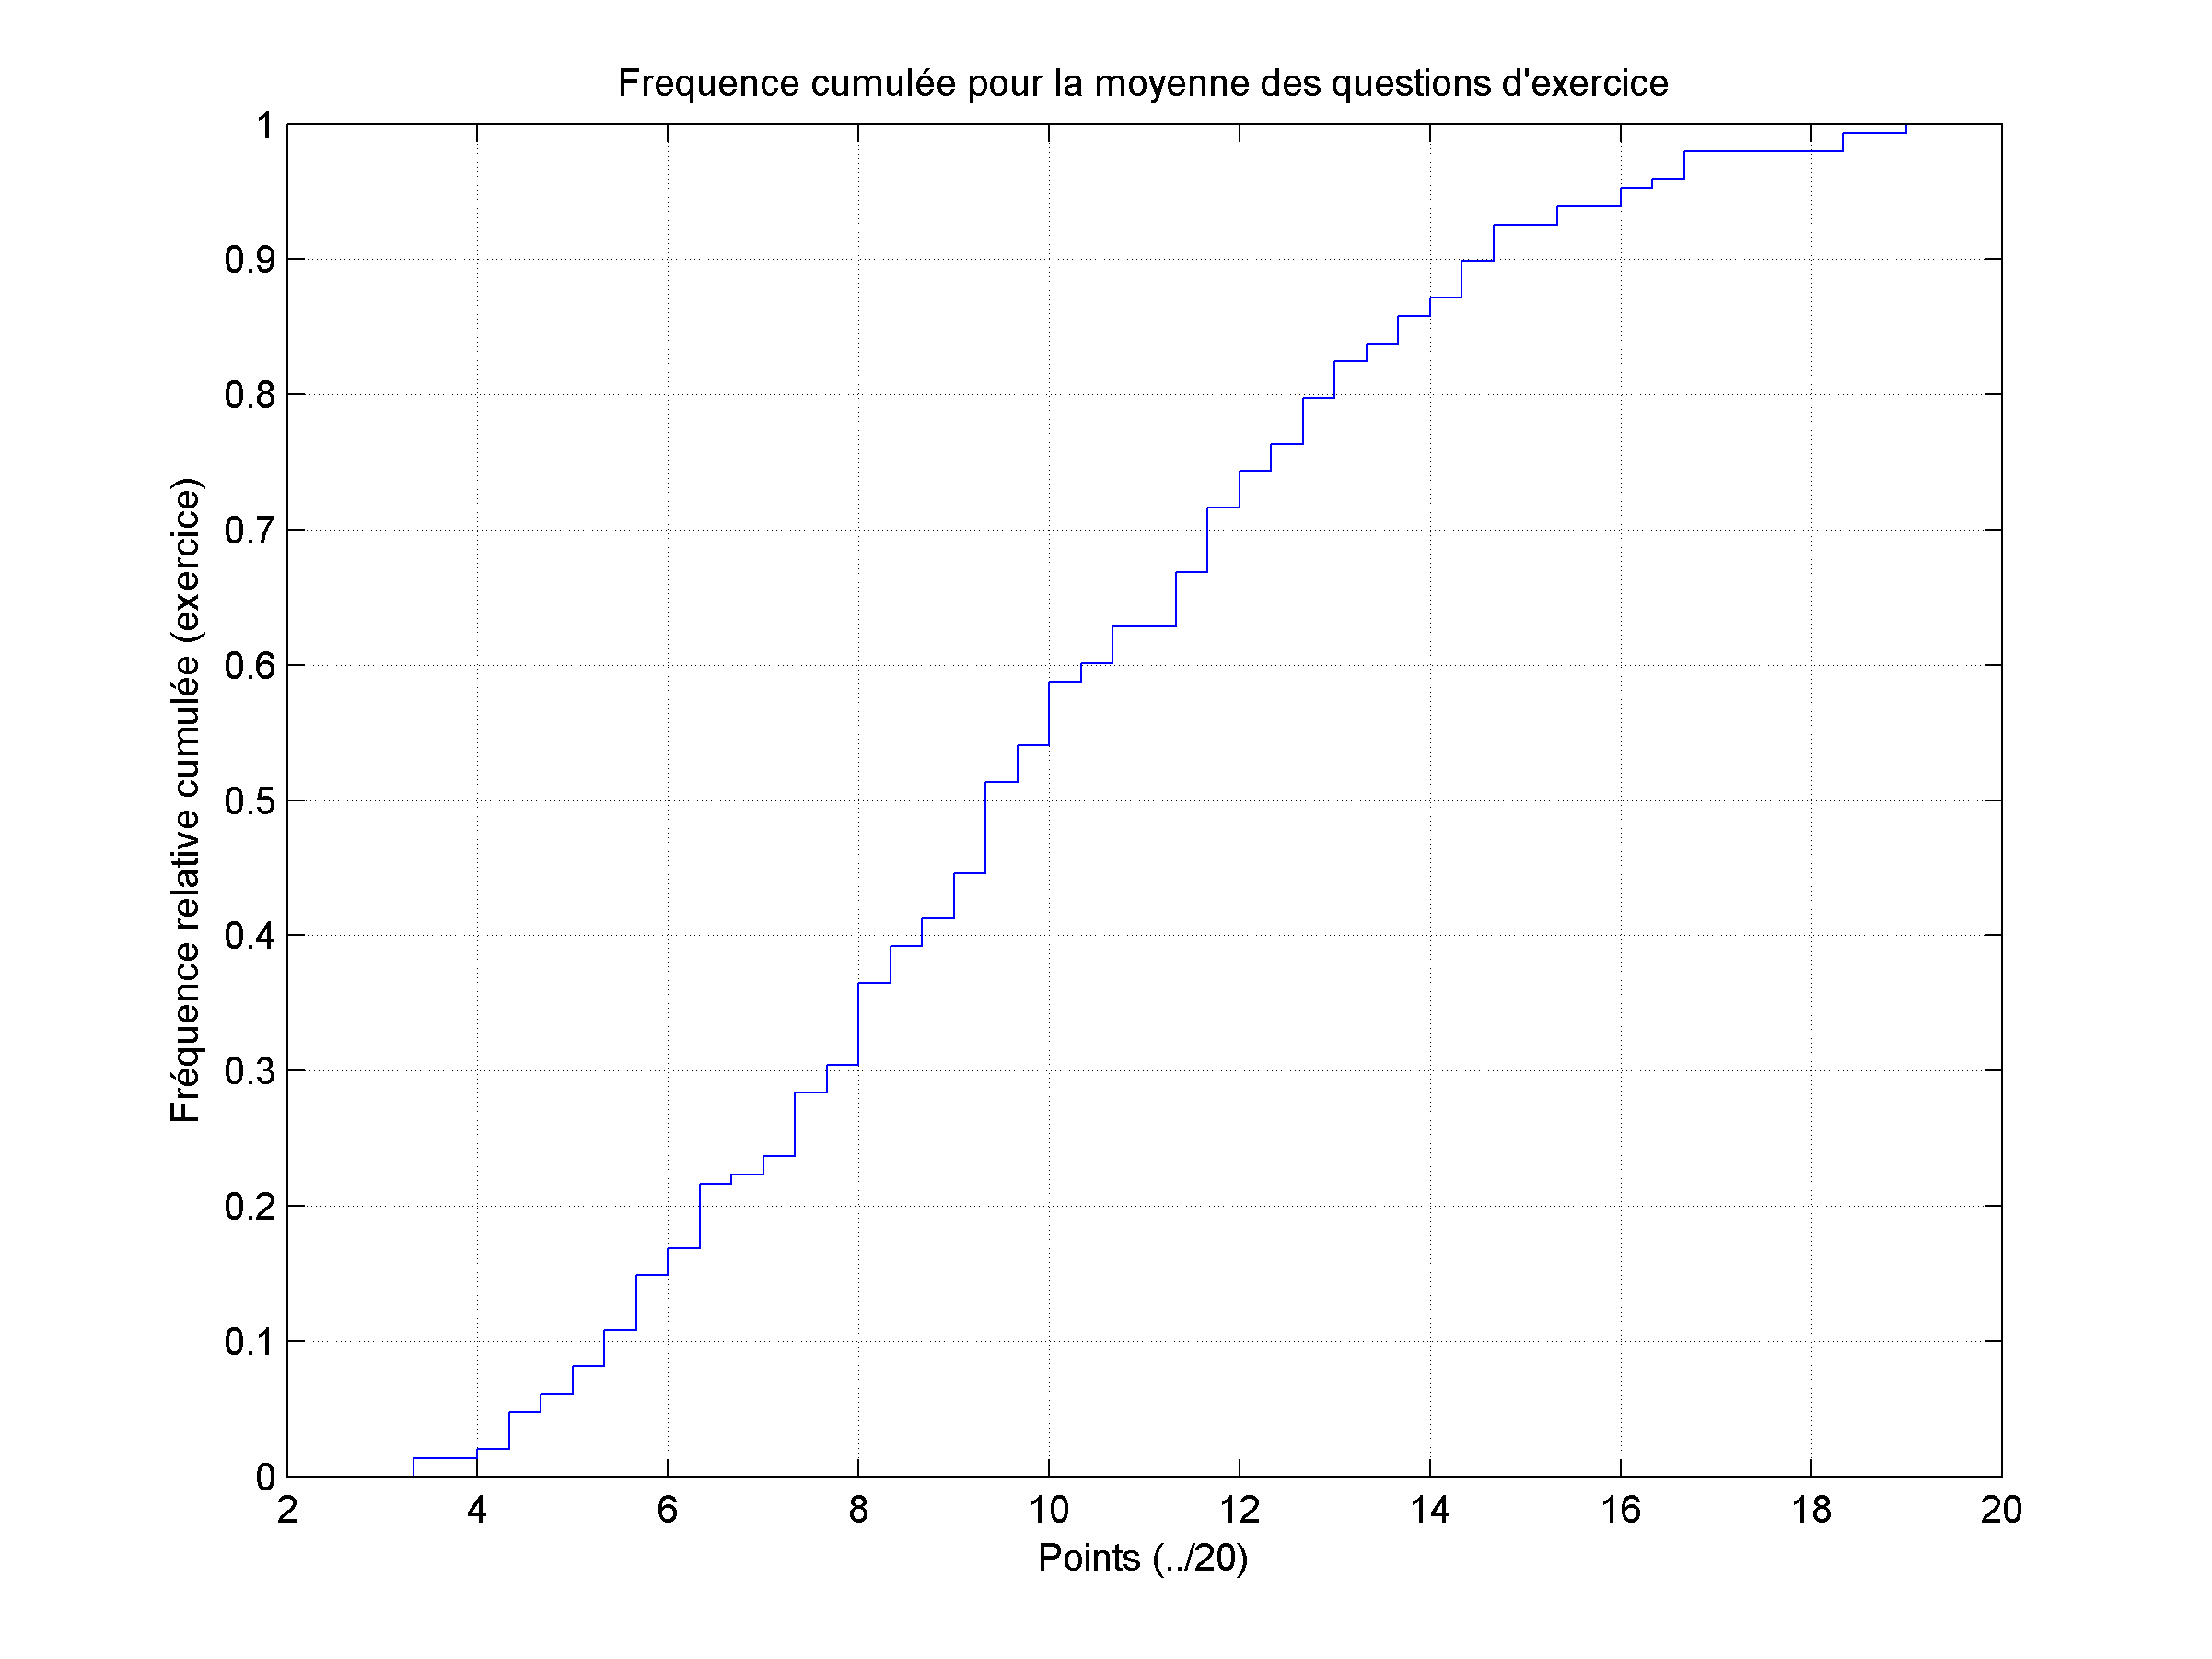
\includegraphics[scale=0.4]{q1d-cdfplot-exer.png}\label{fig:q1d_exer}}
	\caption{Fréquences relatives cumulées}
\end{figure}

\subsection{Point (e)}
Le scatterplot entre les résultats du projet 3 et de la question sur le projet 3 est donné sur la Figure \ref{fig:q1e_scatt}. Le coefficient de corrélation  obtenu est \textbf{0.2106}. En se basant sur ce coefficient de corrélation, on ne peut pas tirer de conclusion de l'influence de la réussite ou non du projet 3 sur la réussite ou non de la question sur le projet 3. En effet, on observe qu'une même proportion de personne ayant réussi le projet 3 (cote $> 10$) a réussi et a raté la question sur le projet 3.
\begin{figure}[!h]
	\center
	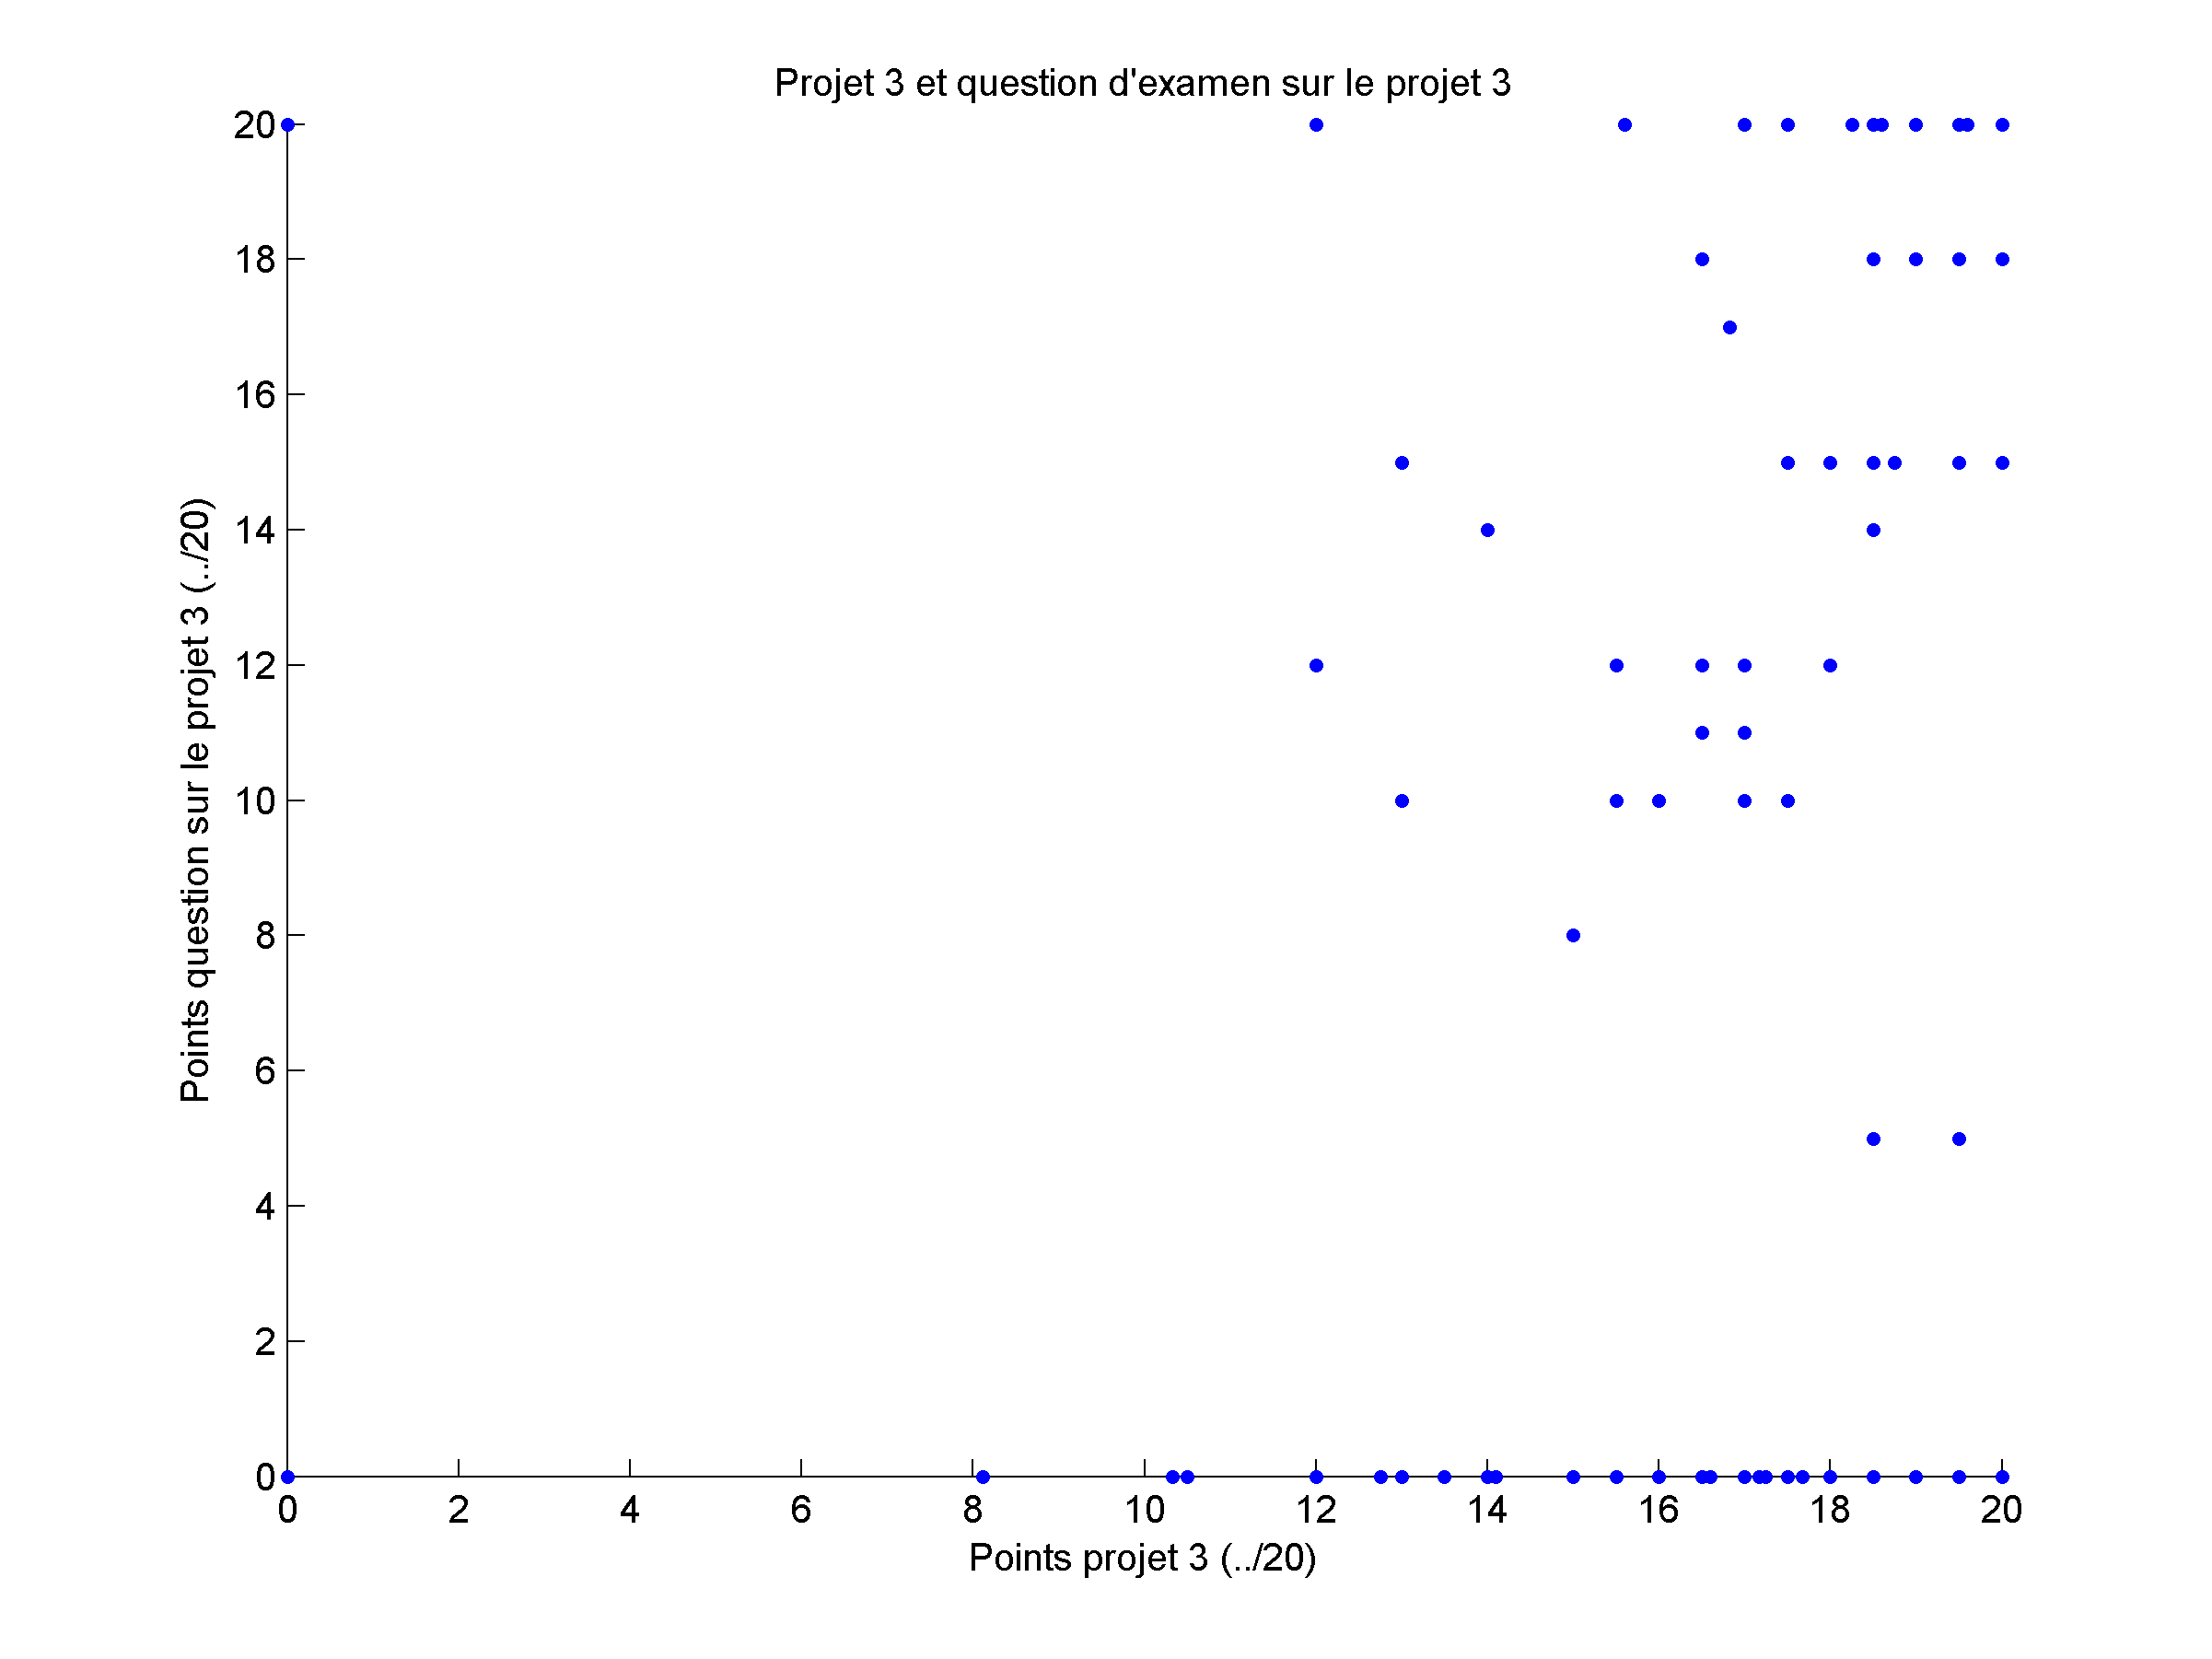
\includegraphics[scale=0.5]{q1d-scatterplot.png}
	\caption{Scatterplot entre les résultats du projet 3 et de la question sur le projet 3}
	\label{fig:q1e_scatt}
\end{figure}

\section{Calcul de statistiques sur échantillons}
\subsection{Remarque sur \texttt{datasample}}
Les échantillons sont calculés avec une implémentation propre de la fonction \texttt{datasample}. Le choix d'implémenter cette fonction est du au fait qu'elle n'est pas présente sur la version R2010a de Matlab.
\paragraph{}
Cette implémentation utilise la fonction \texttt{randi} qui effectue bien un tirage \textit{aléatoire}\footnote{Le tirage étant en fait \textbf{pseudo aléatoire} et basé sur un \textit{seed}, il pourrait être nécessaire d'initialiser ce seed avec une autre valeur que la valeur par défaut afin de ne pas générer des séries de valeurs identiques à chaque ouverture de Matlab. Néamoins, cette opération ne me semble pas nécessaire étant donné l'ampleur de ce projet.} avec remise et permet donc, comme espéré, d'obtenir un échantillon i.i.d. 
\subsection{Point (a)}
\paragraph{(i)} Un échantillon généré aléatoirement à l'aide de \texttt{datasample} est donné dans la Figure \ref{fig:sample1} et les moyennes, médianes et écart types pour les résultats des exercices sont données dans la Table \ref{tab:q2ai_stat1sample}.

\begin{figure}[!h]
	\center
	\textit{15, 19, 21, 24, 42, 63, 72, 81, 94, 118, 119,}\\
 	\textit{121, 135, 136, 136, 142, 142, 143, 143, 144}
	\caption{Index des individus de l'échantillon étudié}
	\label{fig:sample1}
\end{figure}

%
\begin{table}[!h]
	\center
	\begin{tabular}{|c|c|ccc|}
		\hline
		& Exercice & \textbf{Moyenne} & \textbf{Médiane} & \textbf{Ecart type}\\
		\hline
		\multirow{3}{*}{\begin{sideways}\parbox{13.5mm}{\tiny Échantillon}\end{sideways}} & 1 & 9.7500 & 9.0000 & 5.6557\\
		& 2 & 15.600 & 17.000 & 4.7617 \\
		& 3 & 4.6000 & 3.5000 & 4.1218 \\
		\hline
		\multirow{3}{*}{\begin{sideways}\parbox{13.5mm}{\tiny Population}\end{sideways}} & 1 & 8.8243 & 8.0000 & 5.2694\\
		& 2 & 15.0473 & 16.000 & 4.6475\\
		& 3 & 5.5811 & 5.0000 & 4.0919\\
		\hline
	\end{tabular}
	\caption{Moyennes, médianes et écart types pour les exercices}
	\label{tab:q2ai_stat1sample}
\end{table}
%
On observe une légère imprécision sur les statistiques calculées sur base d'un échantillon comparées à celles calculées sur base de la population. En effet, la sélection d'un échantillon provoque une \textbf{perte d'information} par rapport à la population. On constate aussi, en comparant aux statistiques de la population, que l'écart-type varie moins que les autres statistiques. 
\paragraph{(ii)} Dans la continuité de ce qui a été dit au point précédent, on constate que la perte d'information liée à la sélection d'un échantillon entraîne des différences (moins ou plus de données aberrantes, déplacement des quartiles,...) entre les boîtes à moustaches tracées pour la Question 1 et celle donnée sur la Figure \ref{fig:q2a_boxplot}. On peut néanmoins observer que, malgré ces variations évidentes, les boîtes sont positionnées de la même manière qu'à la question 1. Cette observation n'est pas surprenante étant donné que l'échantillon a été tiré de la population qui a donné les premières boîtes.

\begin{figure}[!h]
	\subfigure[Projet 1]{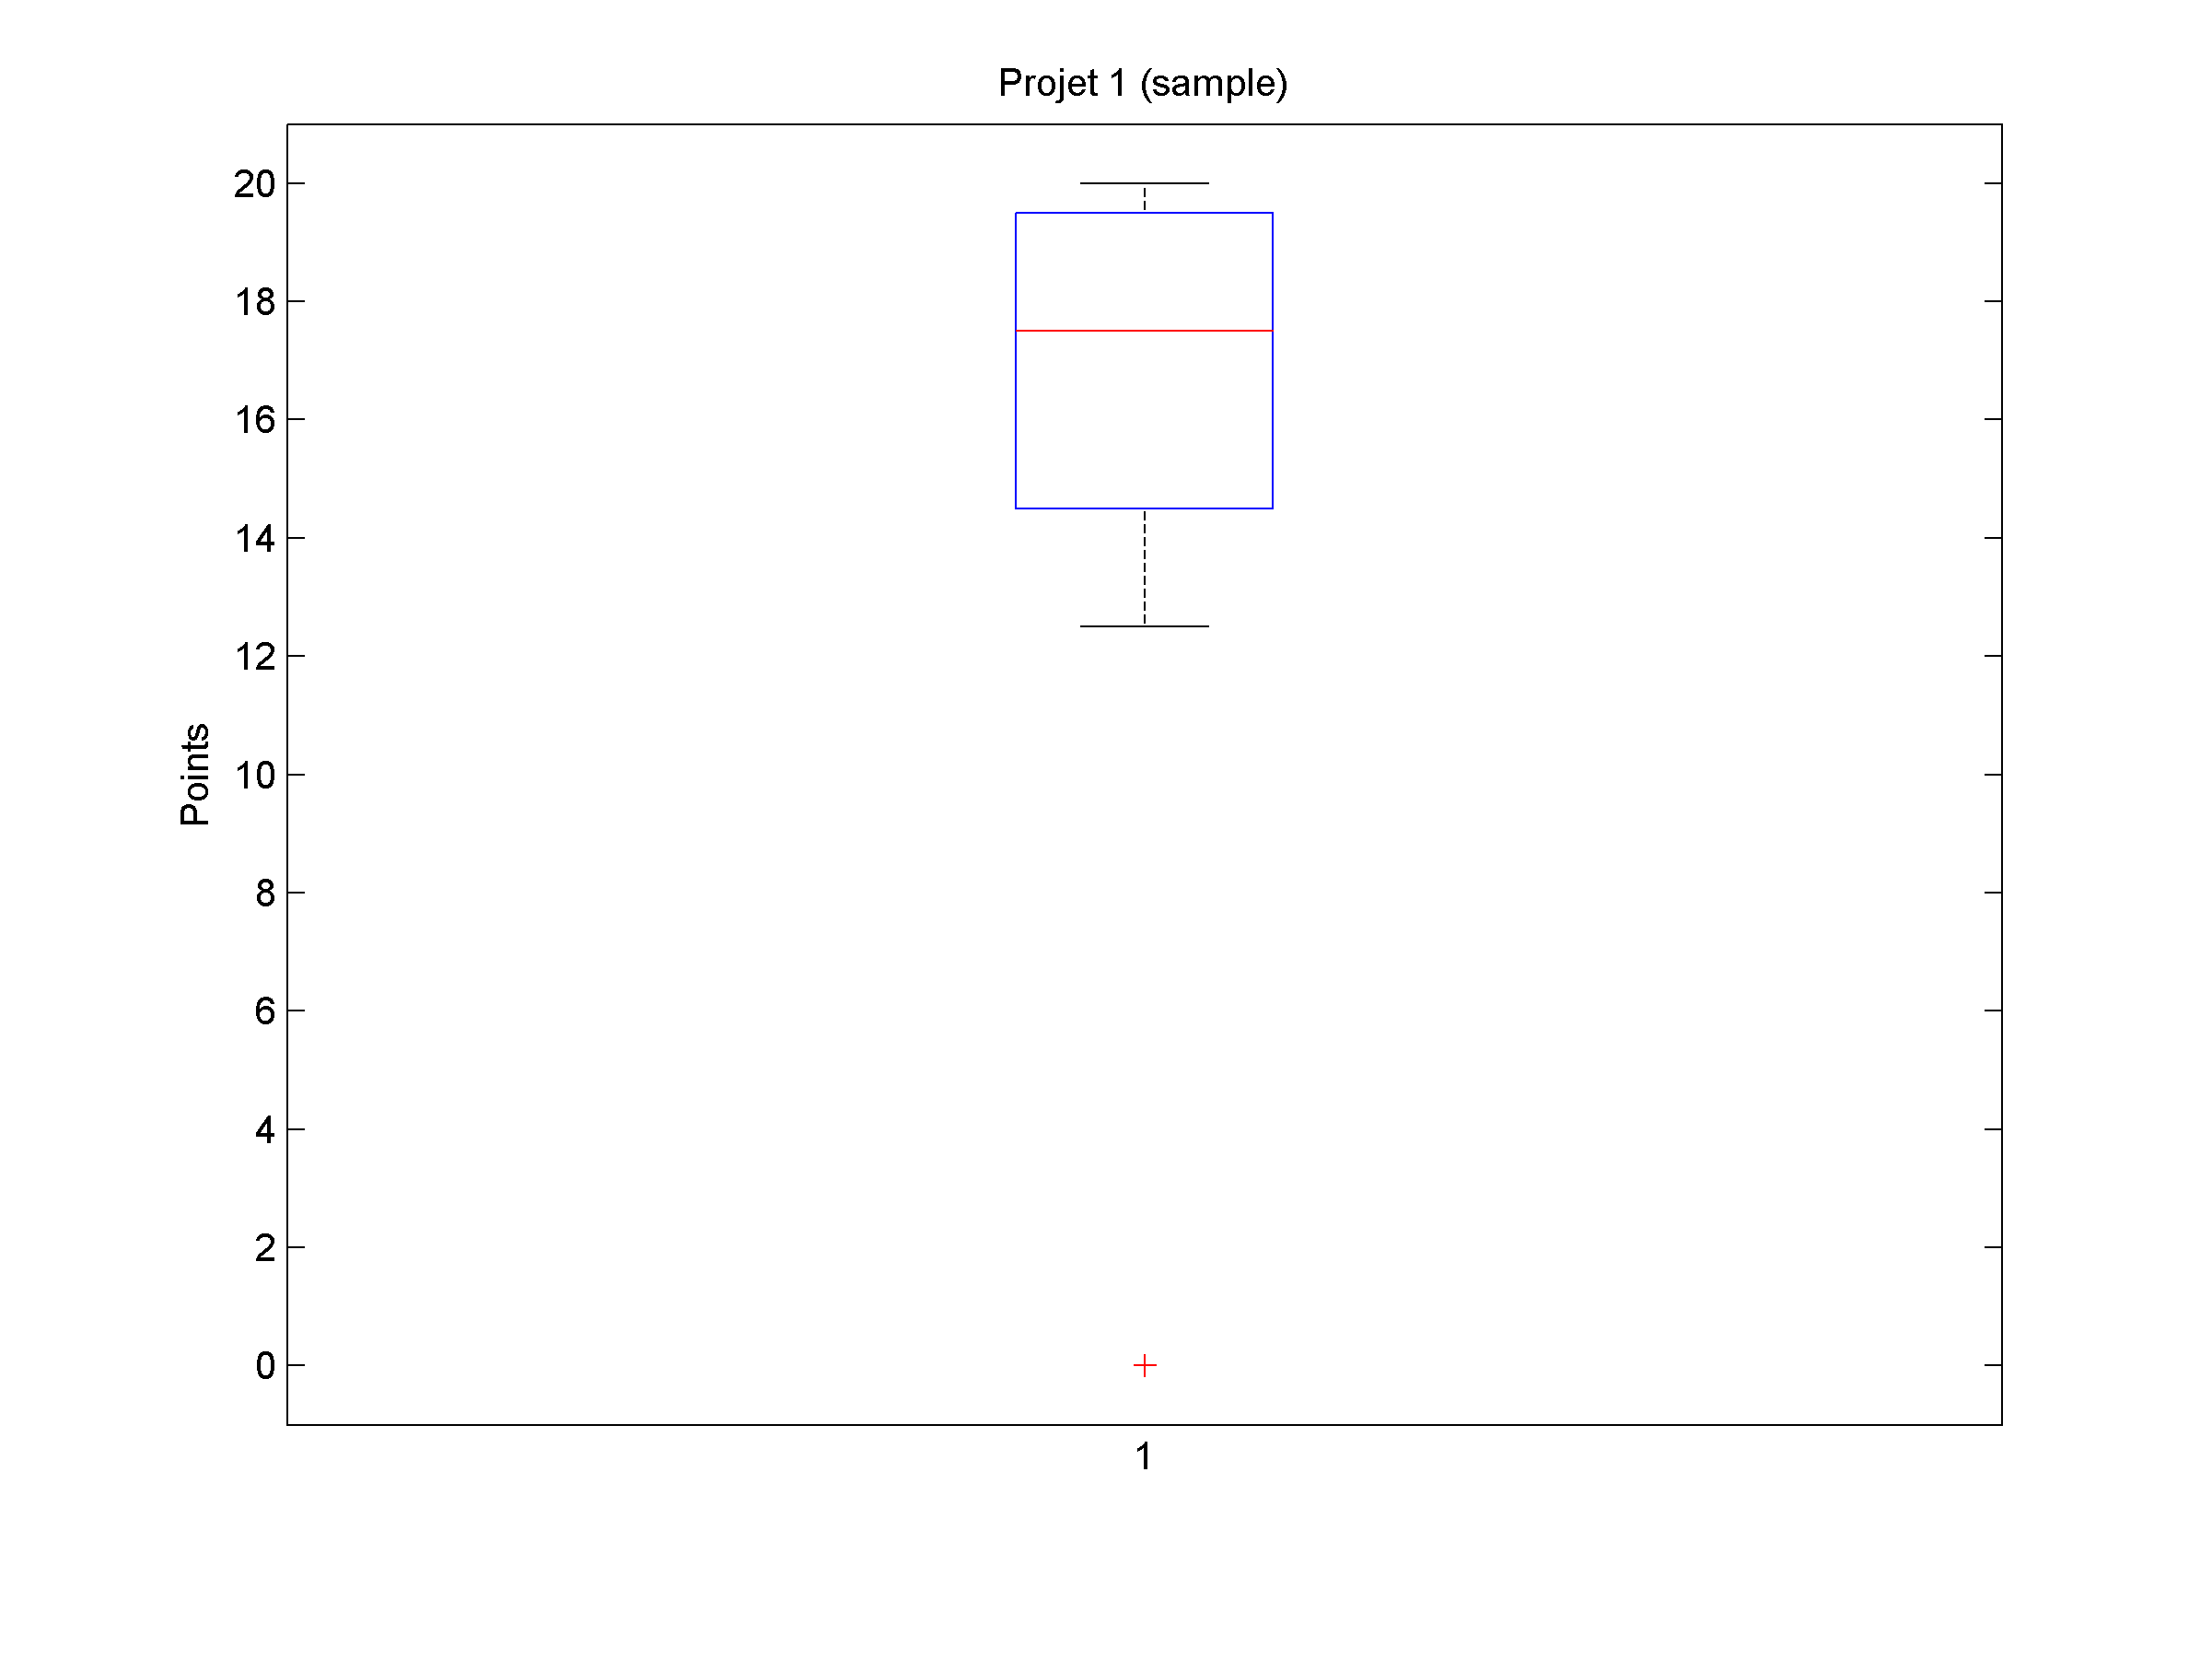
\includegraphics[scale=0.35]{q1aii-proj1.png}}
	\subfigure[Projet 2]{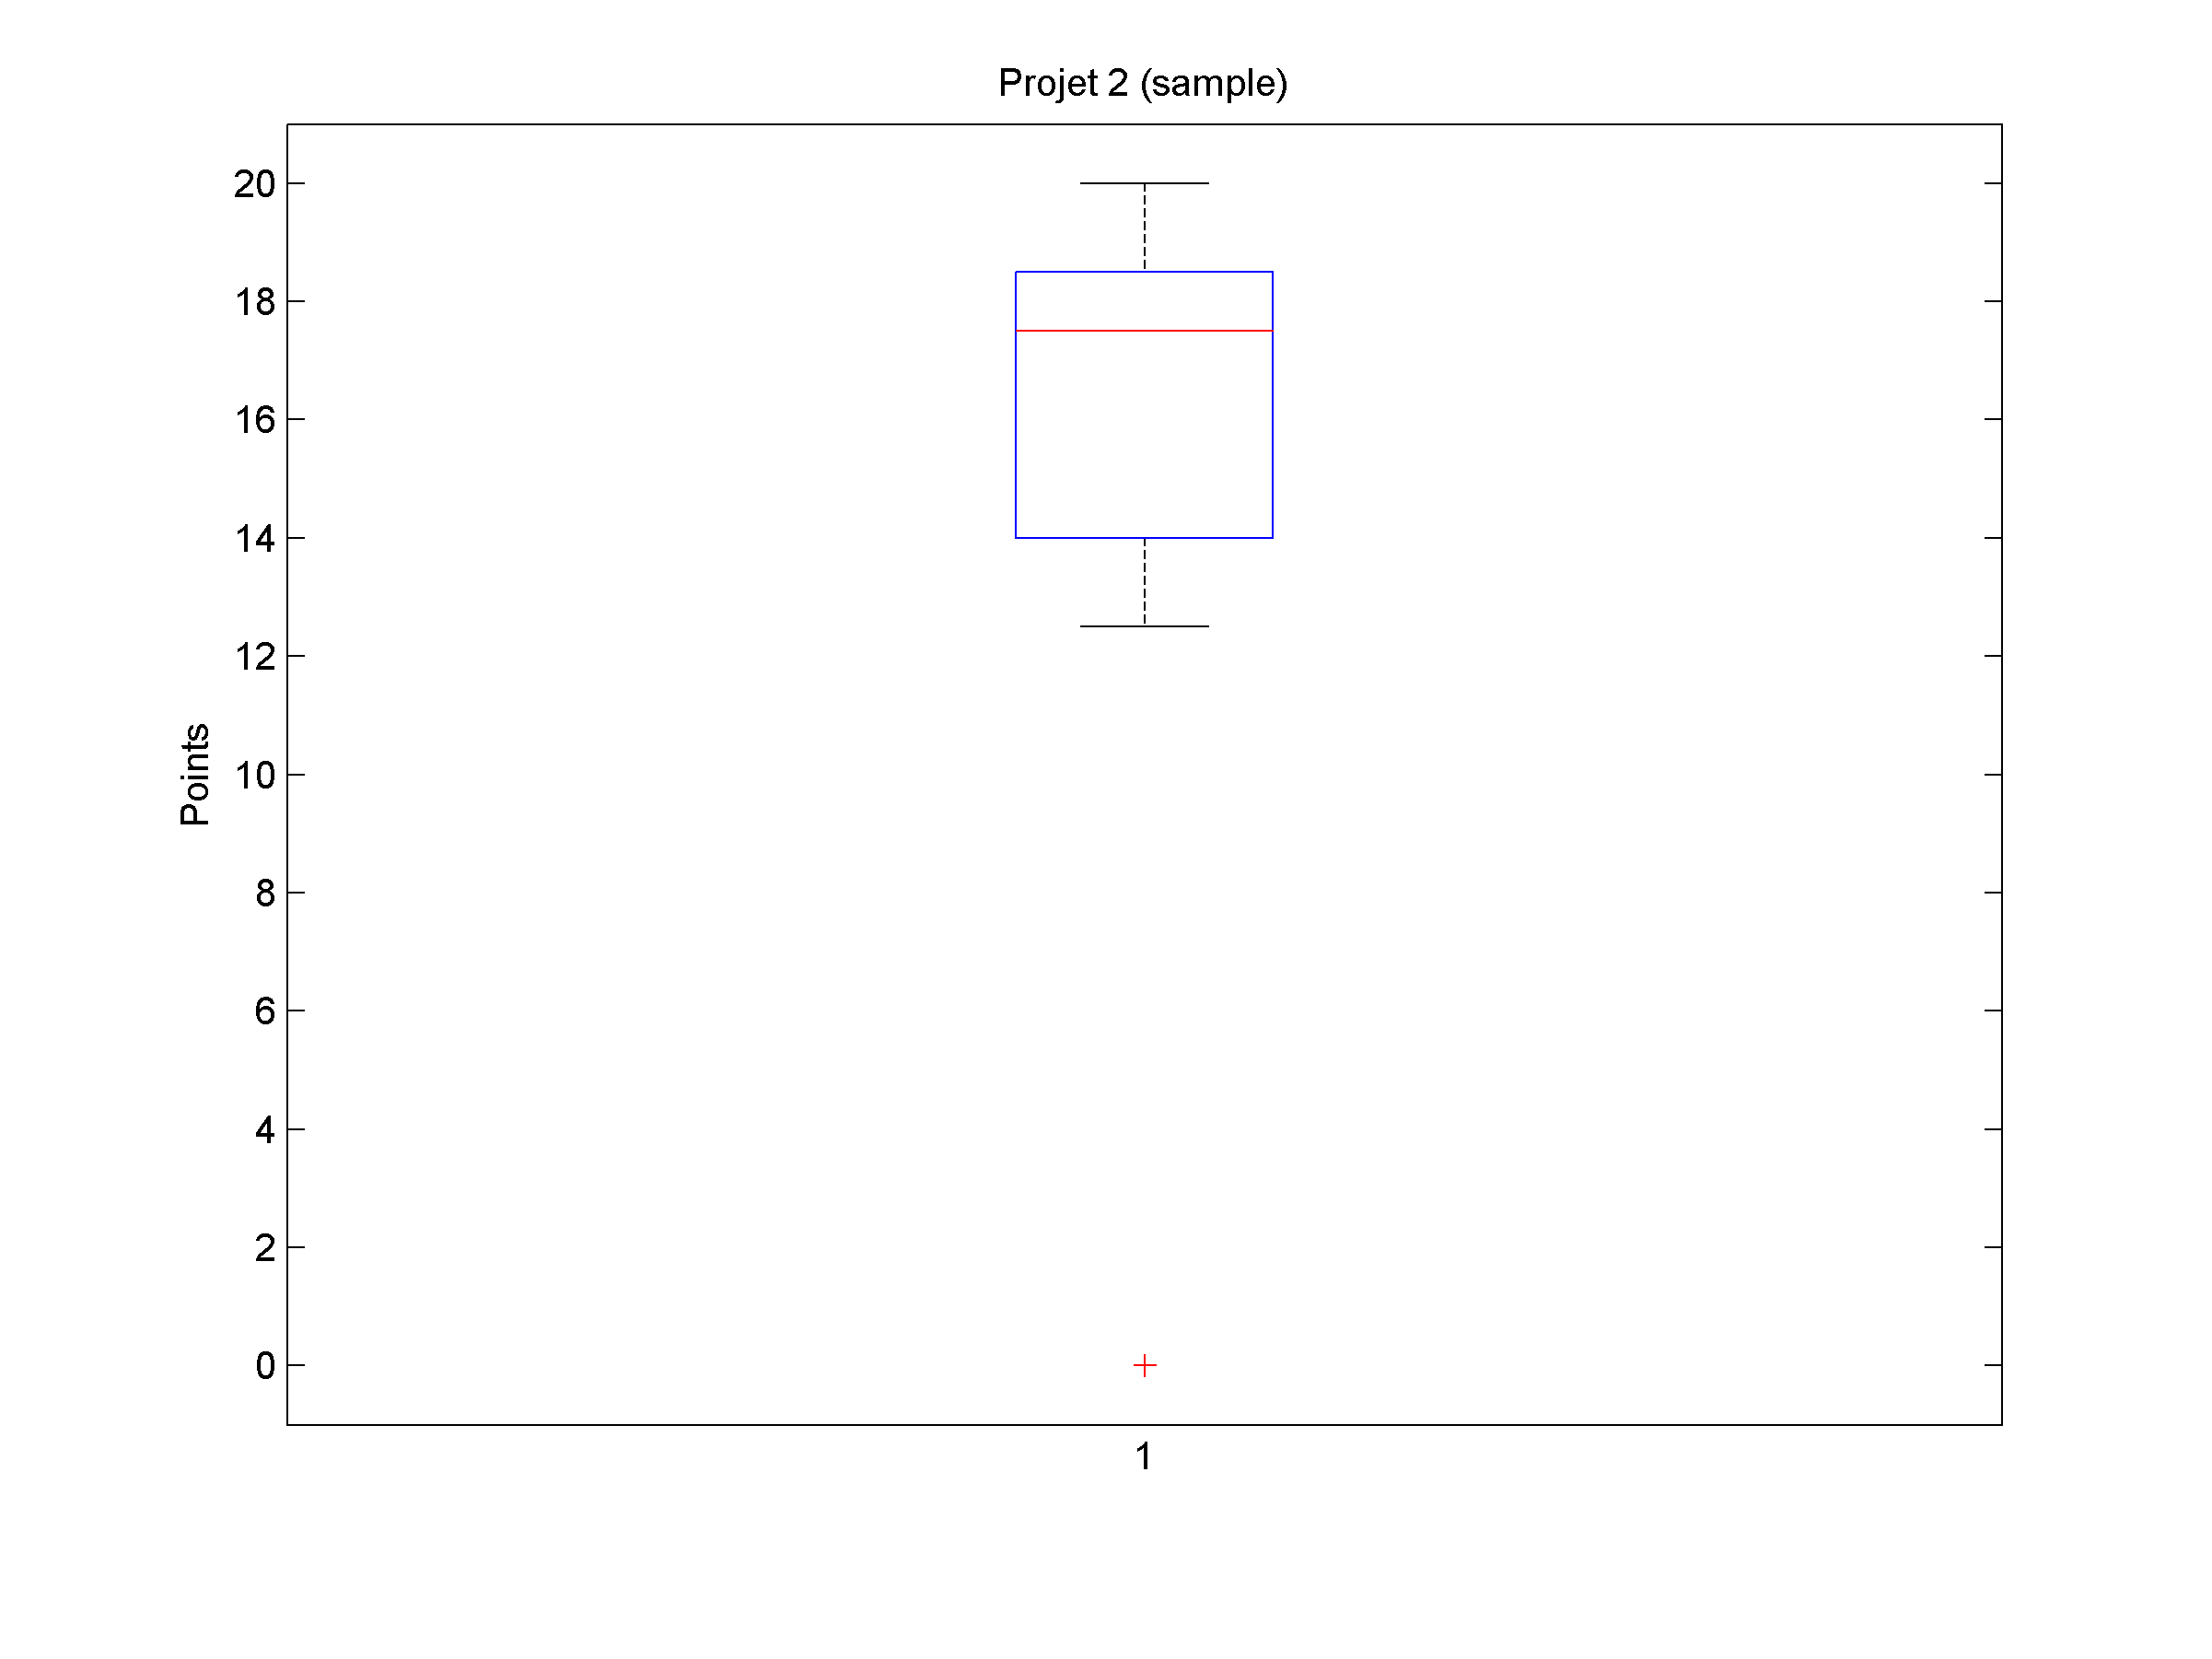
\includegraphics[scale=0.353]{q1aii-proj2.png}}\\
	\subfigure[Projet 3]{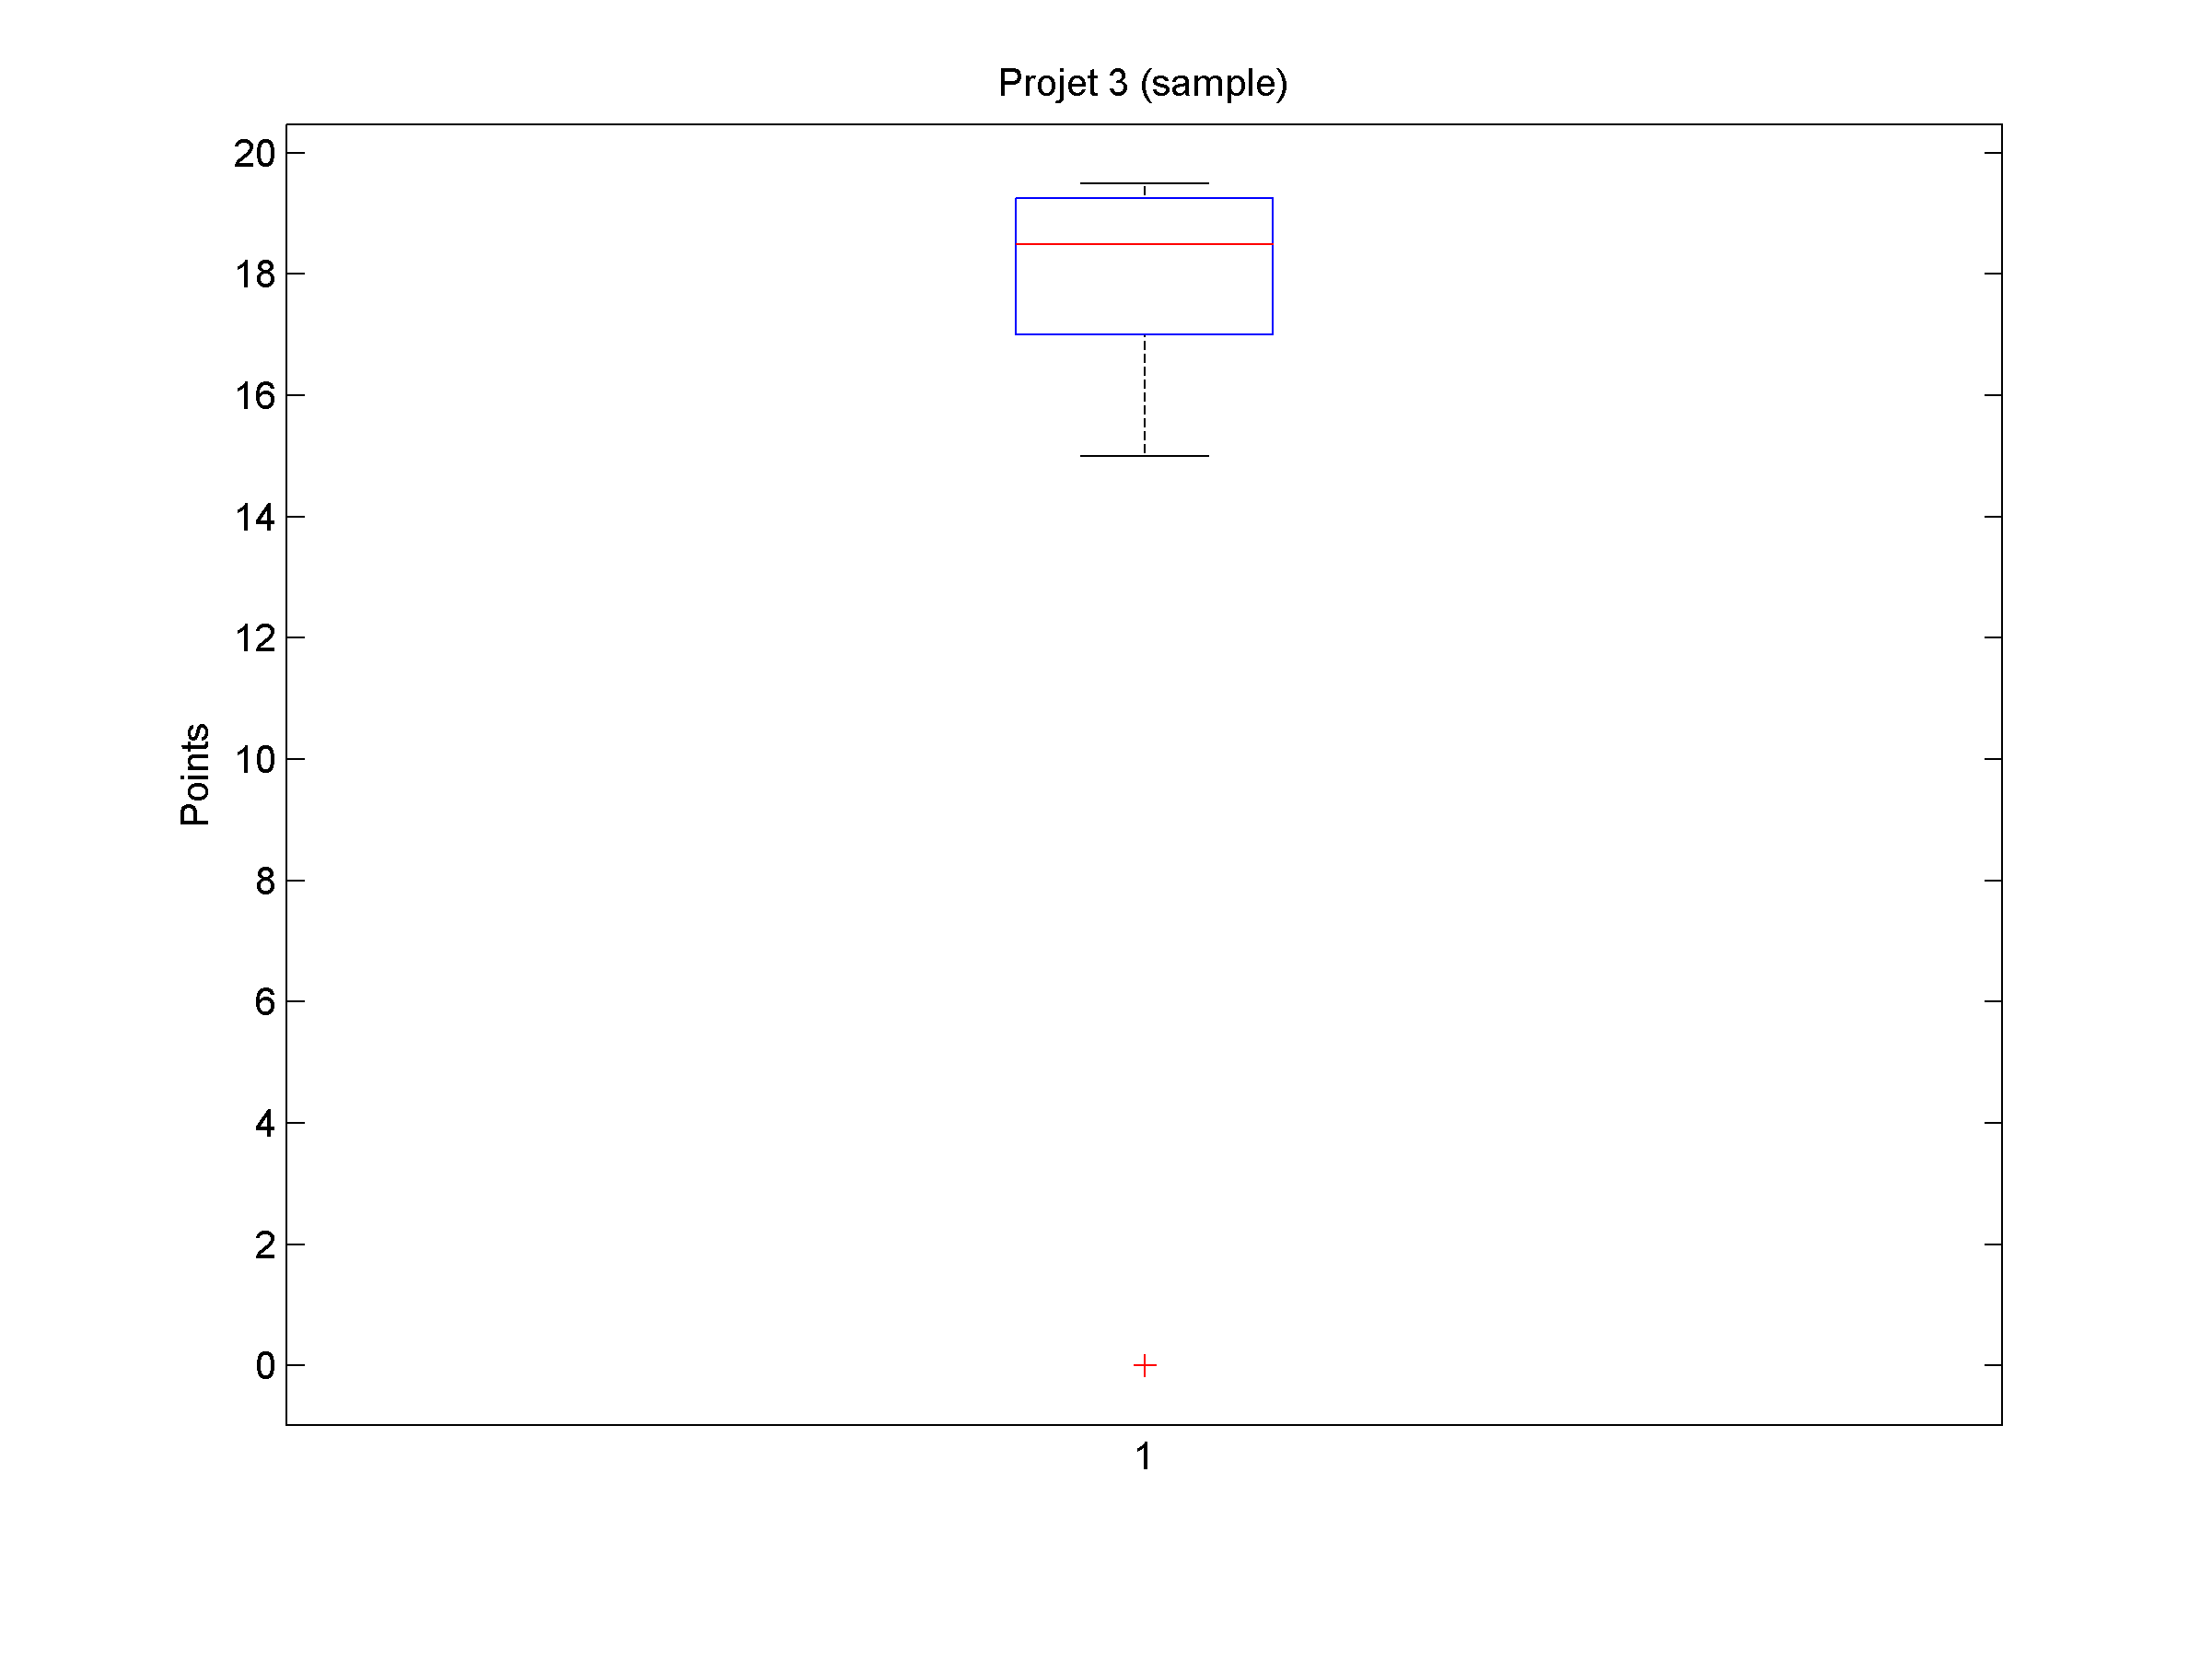
\includegraphics[scale=0.35]{q1aii-proj3.png}}
	\subfigure[Question projet 3]{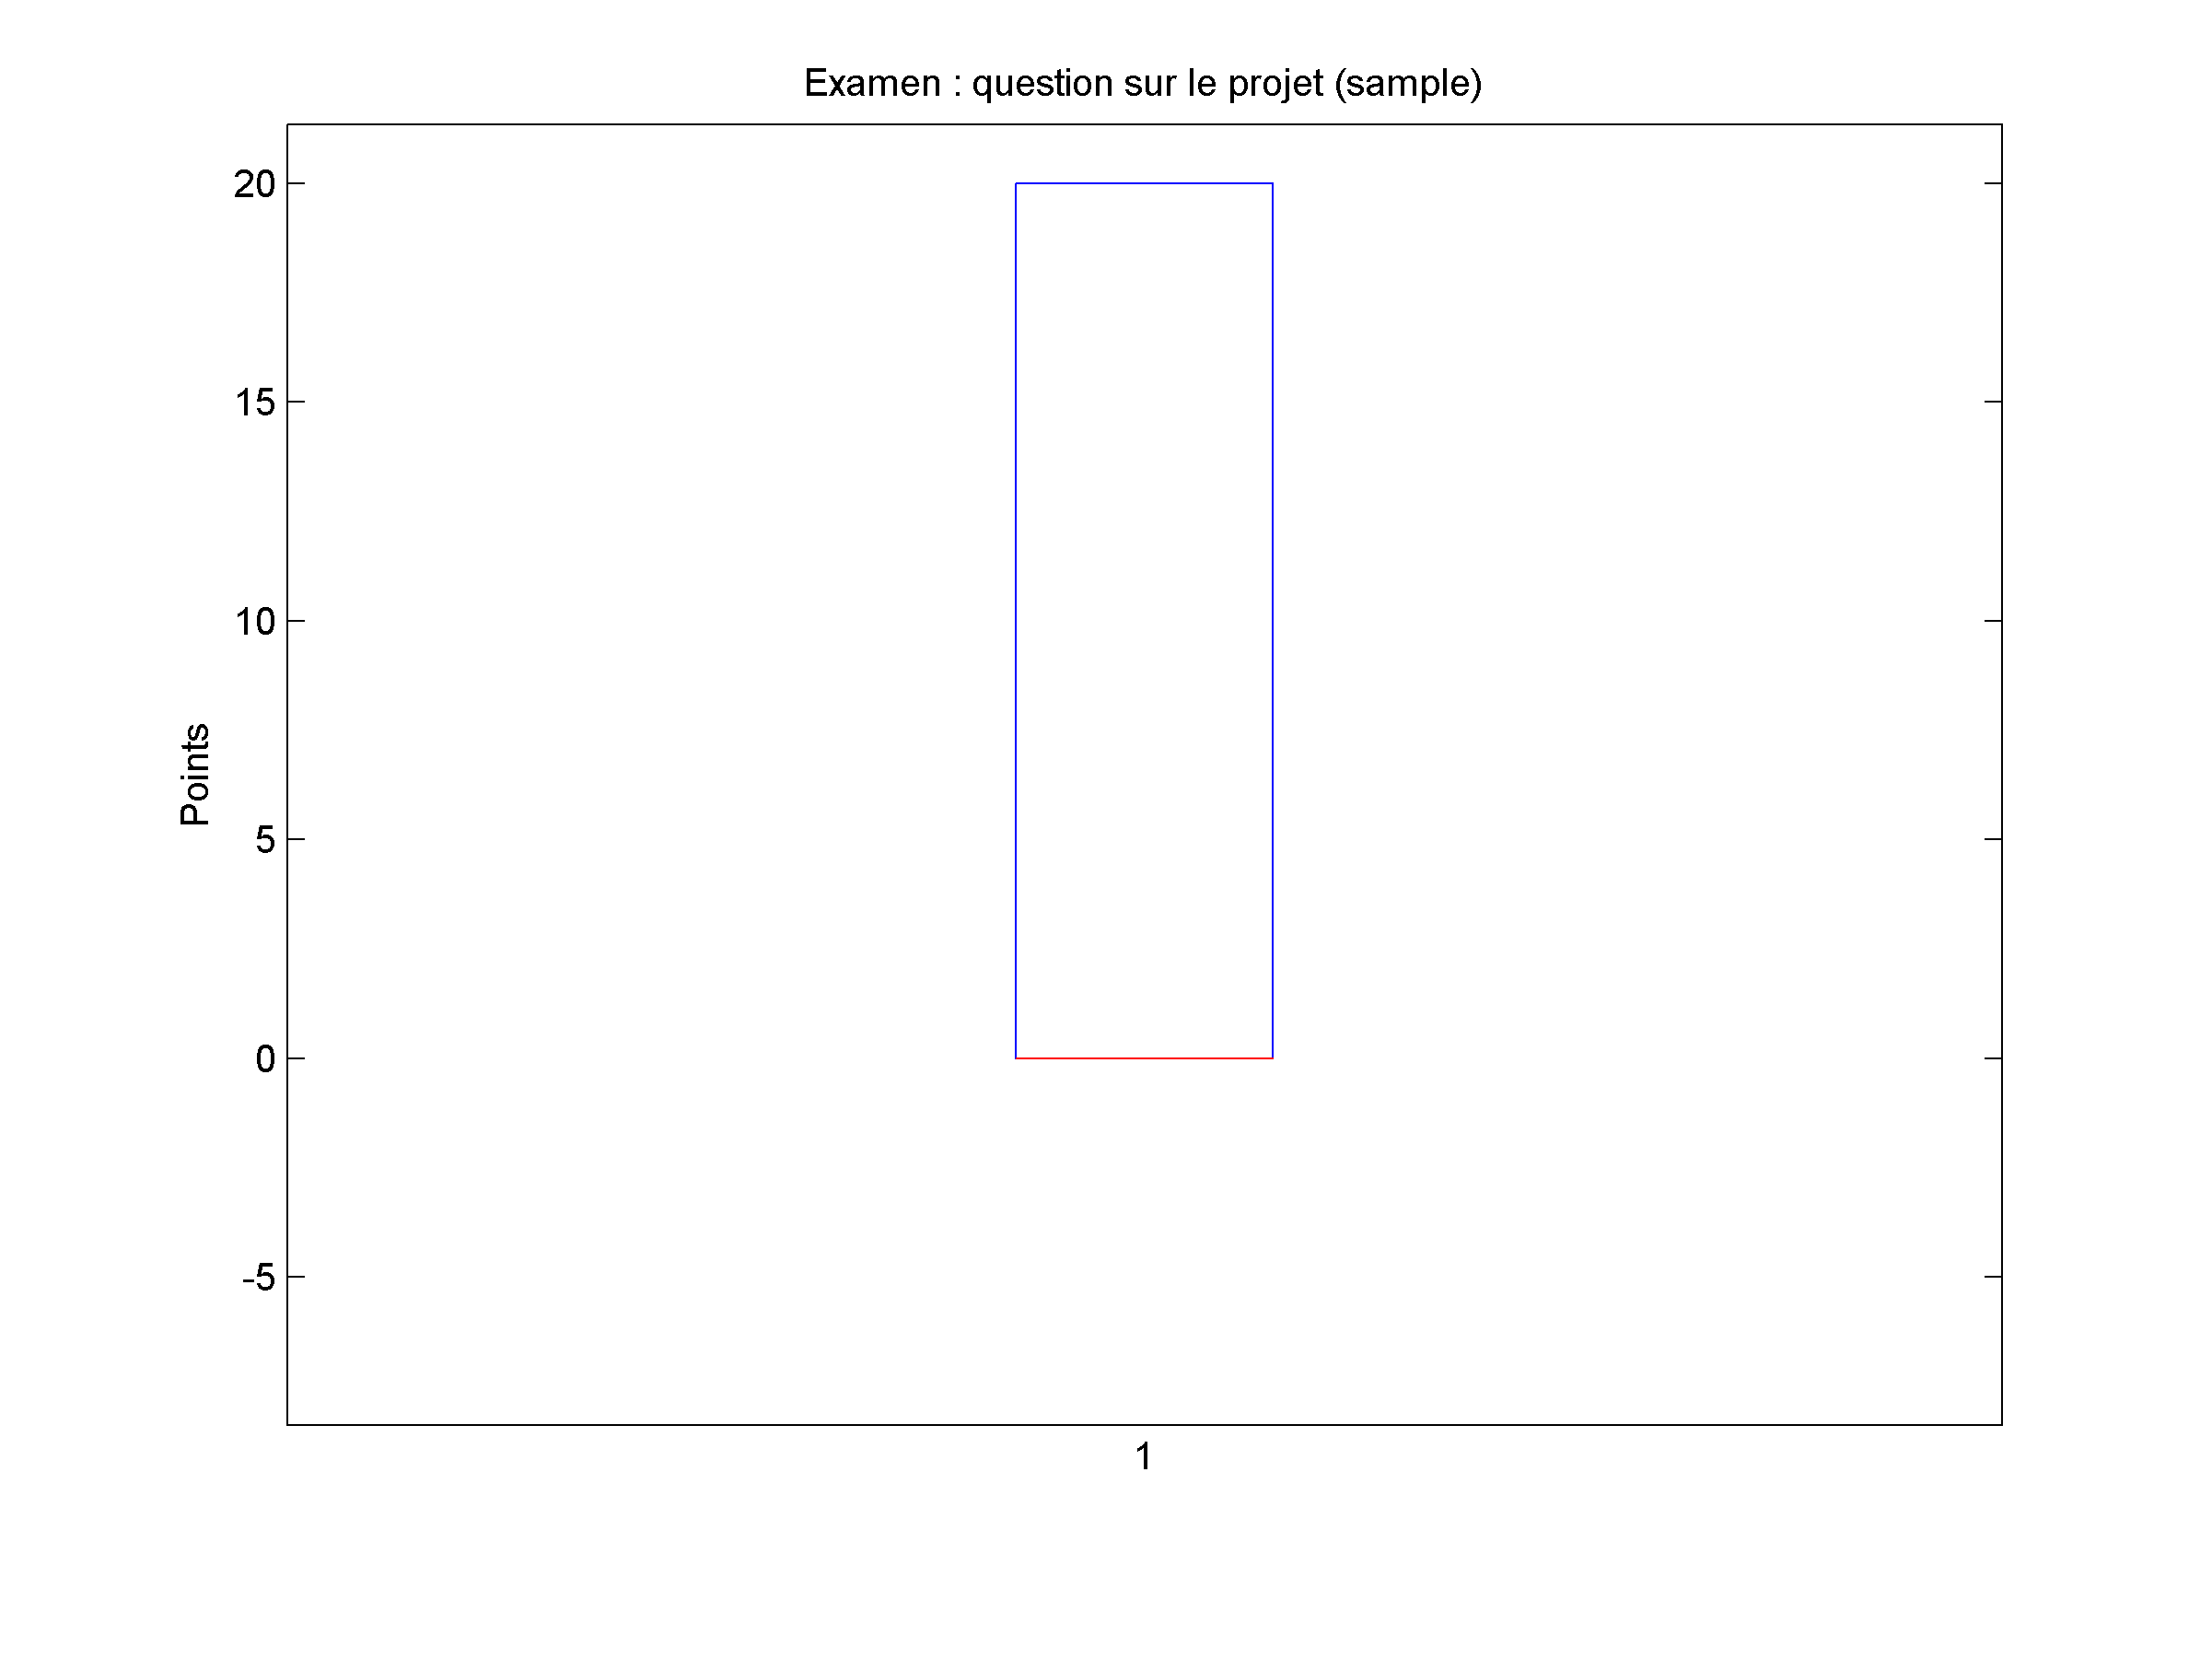
\includegraphics[scale=0.35]{q1aii-exam-proj.png}}
	\caption{Résultat des projets pour l'échantillon}
	\label{fig:q2a_boxplot}
\end{figure}

\paragraph{(iii)} Les courbes des fréquences cumulées pour la moyenne des questions de théorie pour l'échantillon et la population sont données sur la Figure \ref{fig:q2iii_freq}. On constate que la fonction relative à l'échantillon contient moins de marches que celle de la population. Encore une fois, cette observation n'est pas surprenante étant donné que le nombre d'individus est beaucoup plus petit dans le premier cas. De ce fait, la fonction est moins proche de la courbe théorique (distribution normale) que la courbe de la population.
\paragraph{}
La distance de Kolmogorov-Smirnov entre les deux courbes est calculée à l'aide de la fonction \texttt{kstest2}. La distance de K-S entre les fonctions pour l'échantillon et la population est $\mathbf{0.0986}$. Cette valeur, qui est relativement faible, indique que les deux distributions suivent probablement de la même loi de probabilité.

\begin{figure}[!h]
	\center
	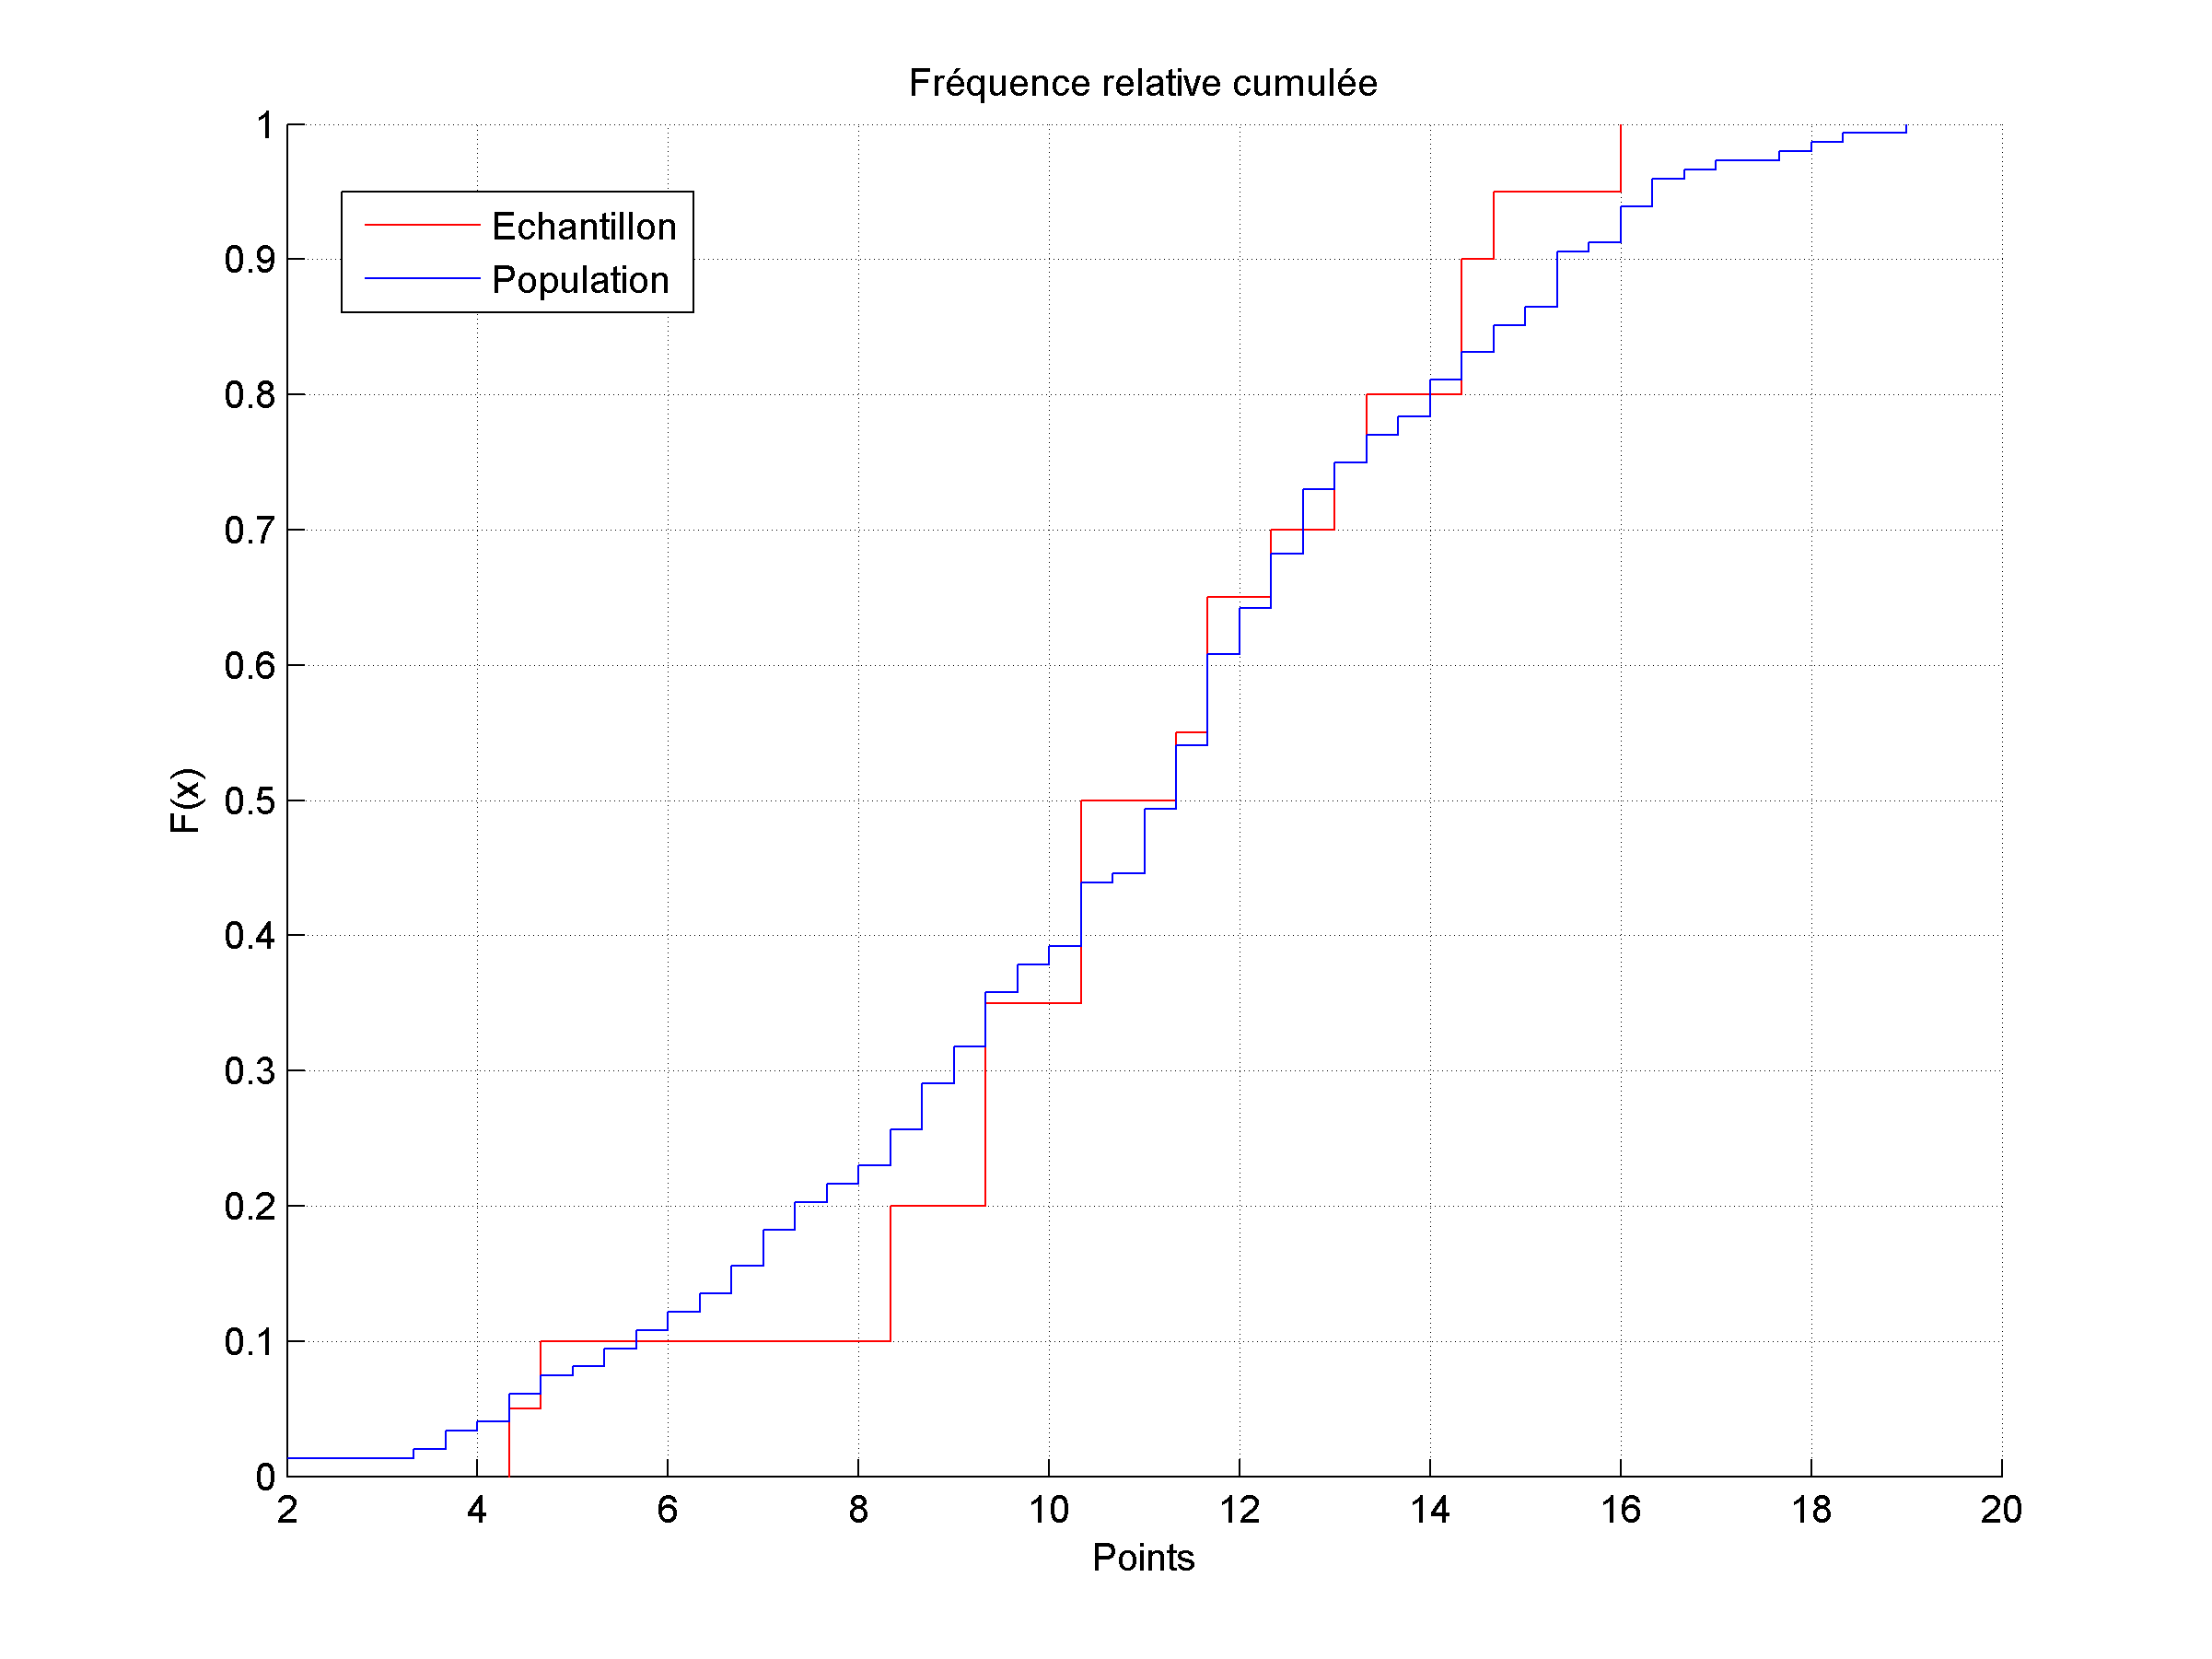
\includegraphics[scale=0.5]{q1aiii-freqcum.png}
	\caption{Fréquences cumulées pour la moyenne des questions de théorie}
	\label{fig:q2iii_freq}
\end{figure}

\subsection{Point (b)}
Les histogrammes pour les sous-questions $(i)$, $(ii)$ et $(iii)$ sont donnés sur la Figure \ref{fig:q2b_stat_100sample}.
\paragraph{(i)} La moyenne des moyennes (pour l'exercice 1) est $\mathbf{8.8645}$. Cette moyenne est \textbf{proche} de la moyenne pour la population et bien plus précise que la valeur obtenue avec un seul échantillon. 
On peut expliquer cette précision accrue par le fait que l'augmentation du nombre d'échantillon a \textit{atténué la perte d'information}. En effet, pour 100 échantillons le nombre d'individus différents sondés a fortement augmenter.
\paragraph{} L'allure de l'histogramme rappelle la \textbf{loi normale}. En effet, on constate une accumulation d'individus autour de la moyenne de cette variable et une décroissance de la fonction de part et d'autre de cette moyenne.
\paragraph{(ii)} La moyenne des médianes est $\mathbf{8.2250}$. Cette valeur est, comme au point $2.b.(i)$, plus précise que celle trouvée pour un seul échantillon. 
\paragraph{}
On constate, à nouveau, l'accumulation des médianes autour de la moyenne des médianes mais la décroissance de part et d'autre de la moyenne est moins évidente que pour la moyenne des moyennes.  
\paragraph{(iii)} La moyenne des écart-types est $\mathbf{5.3321}$. Encore une fois, cette valeur est plus précise que pour un seul échantillon. 
\paragraph{}
Pour ce qui est du graphe, on retrouve une loi normale sur base des mêmes observations que celles énoncés aux points précédents.
\paragraph{(iv) et (v)} Les histogrammes des distances de Kolmogorov-Smirnov entre les fonctions de fréquences cumulées des exercices pour 100 échantillons par rapport à la population sont donnés sur la Figure \ref{fig:q2b_ks_100sample}. 
\paragraph{}
L'allure des histogrammes rappelle une loi normale. La distance de K-S pour un échantillon aléatoire et la population dont l'échantillon est extrait évolue selon une loi normale.

\begin{figure}[!h]
	\center
	\subfigure[Moyenne]{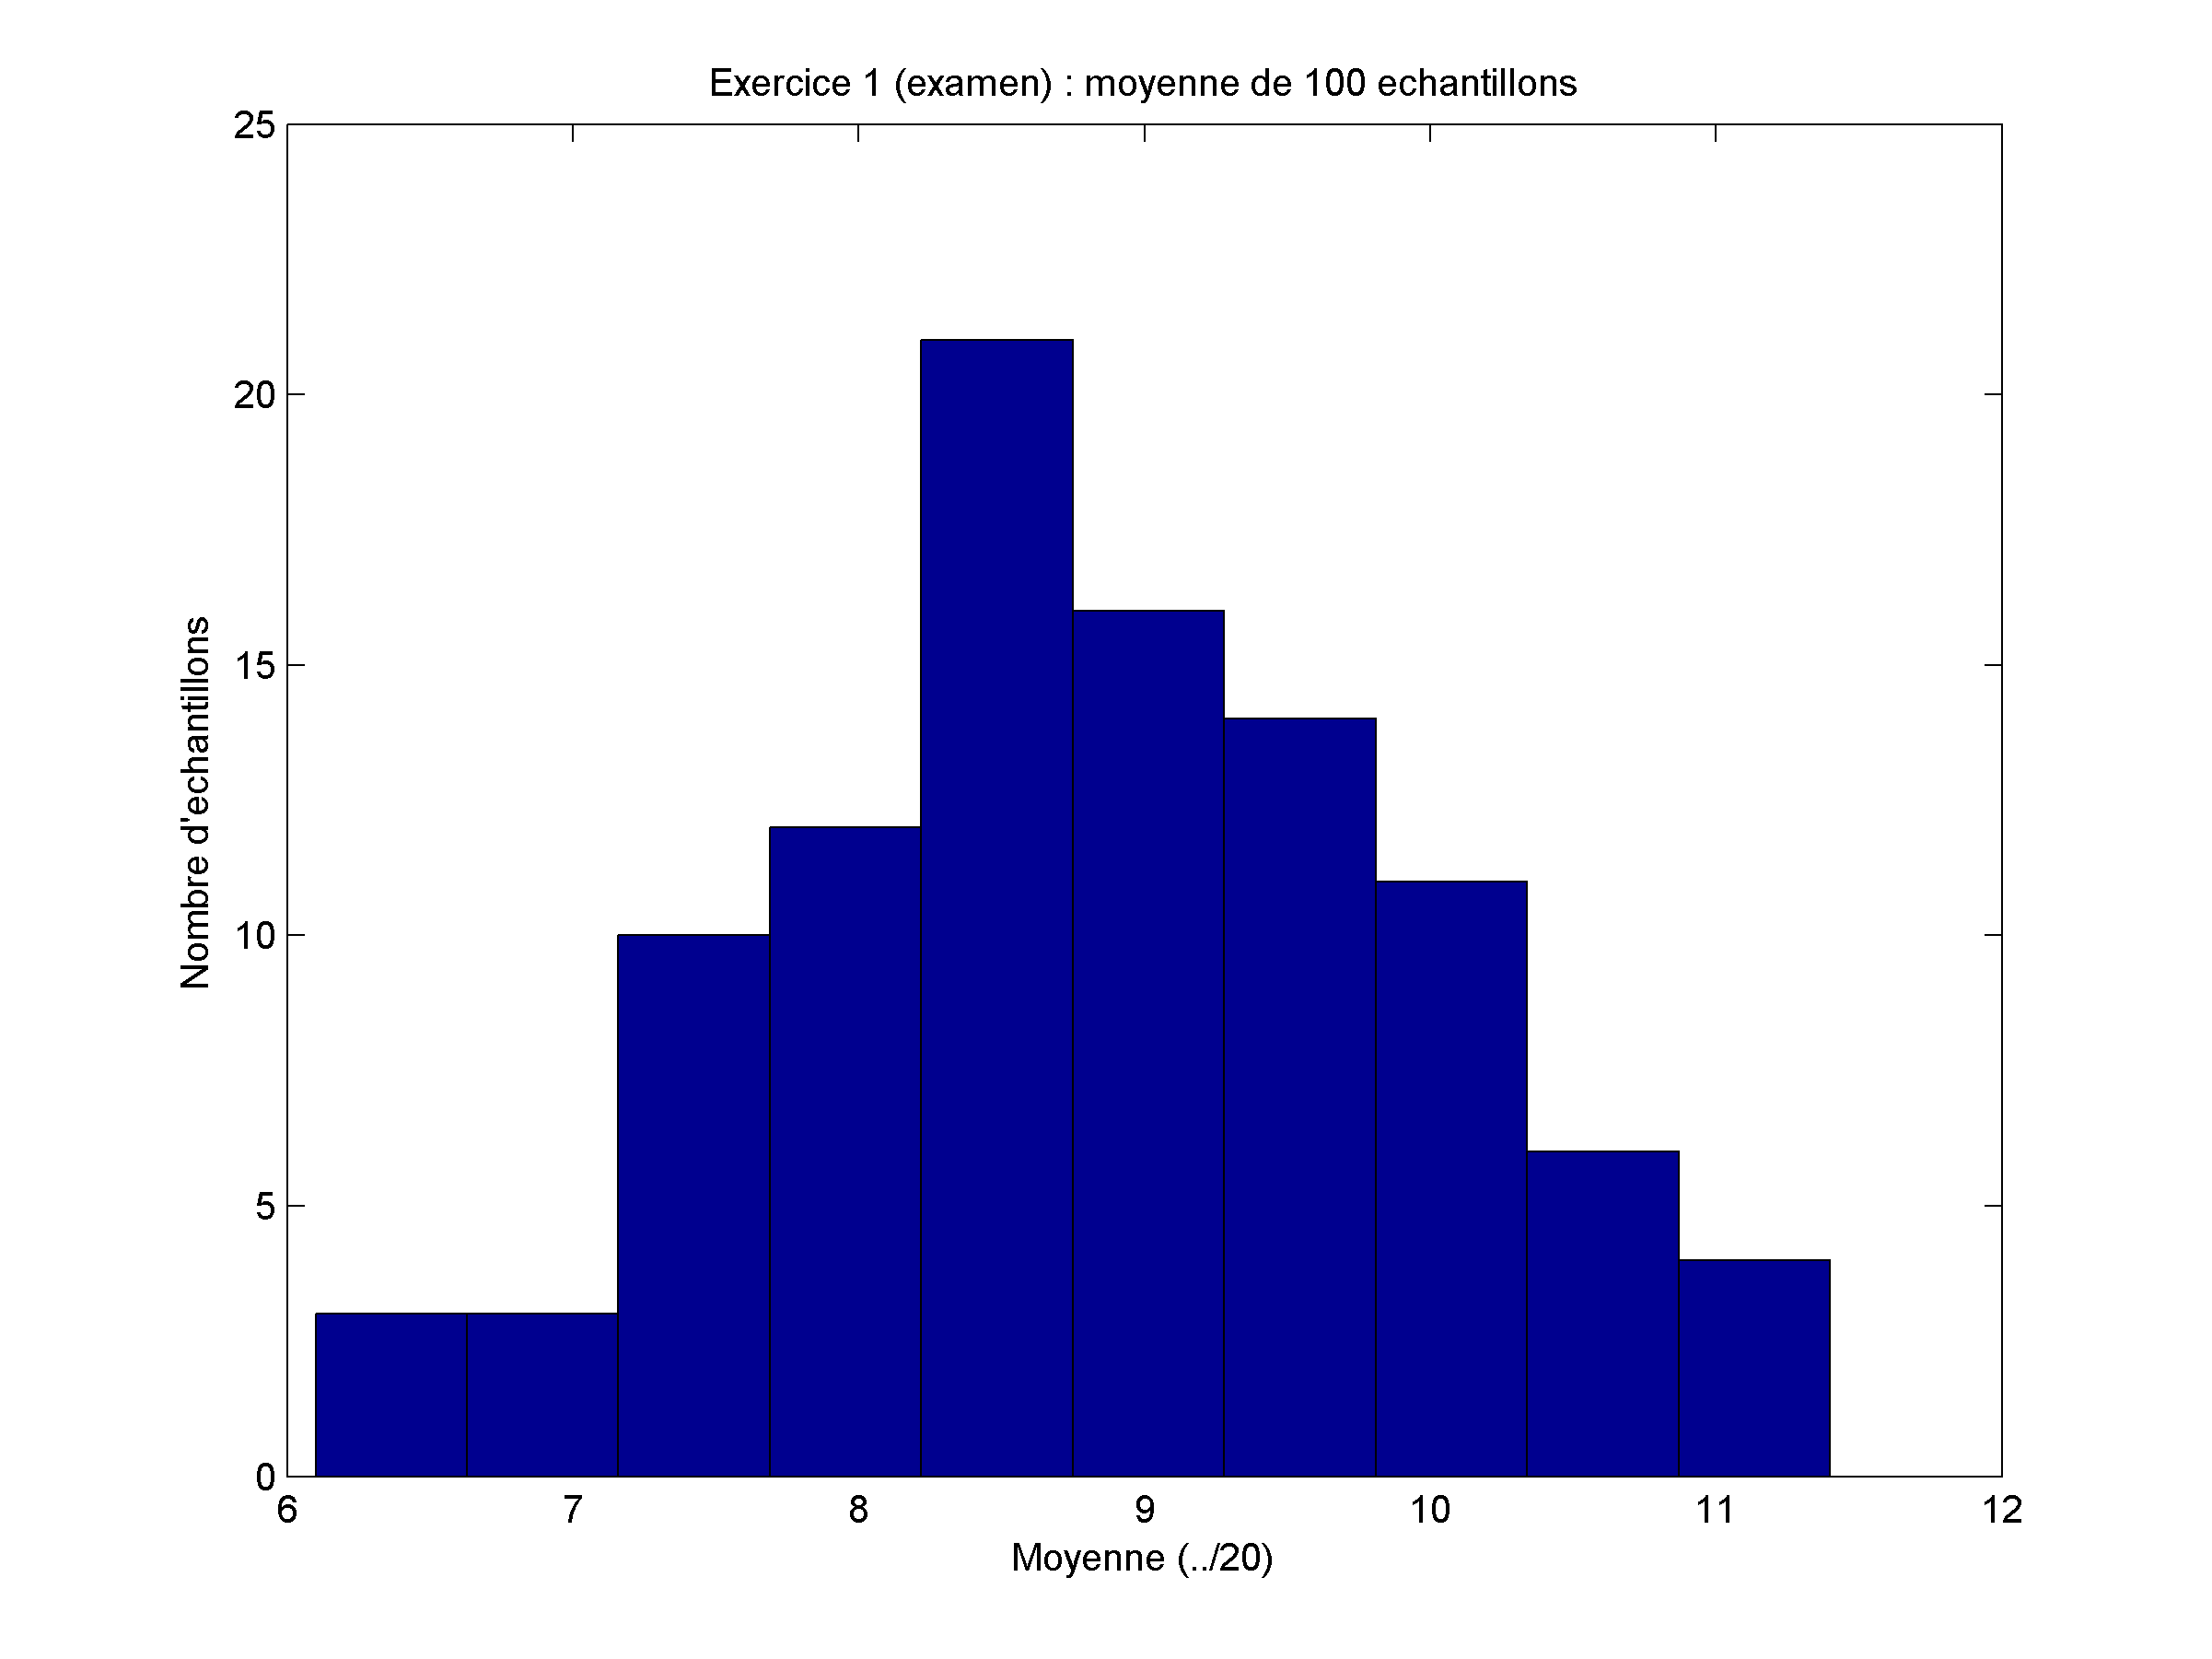
\includegraphics[scale=0.35]{q2b-mean.png}}
	\subfigure[Médiane]{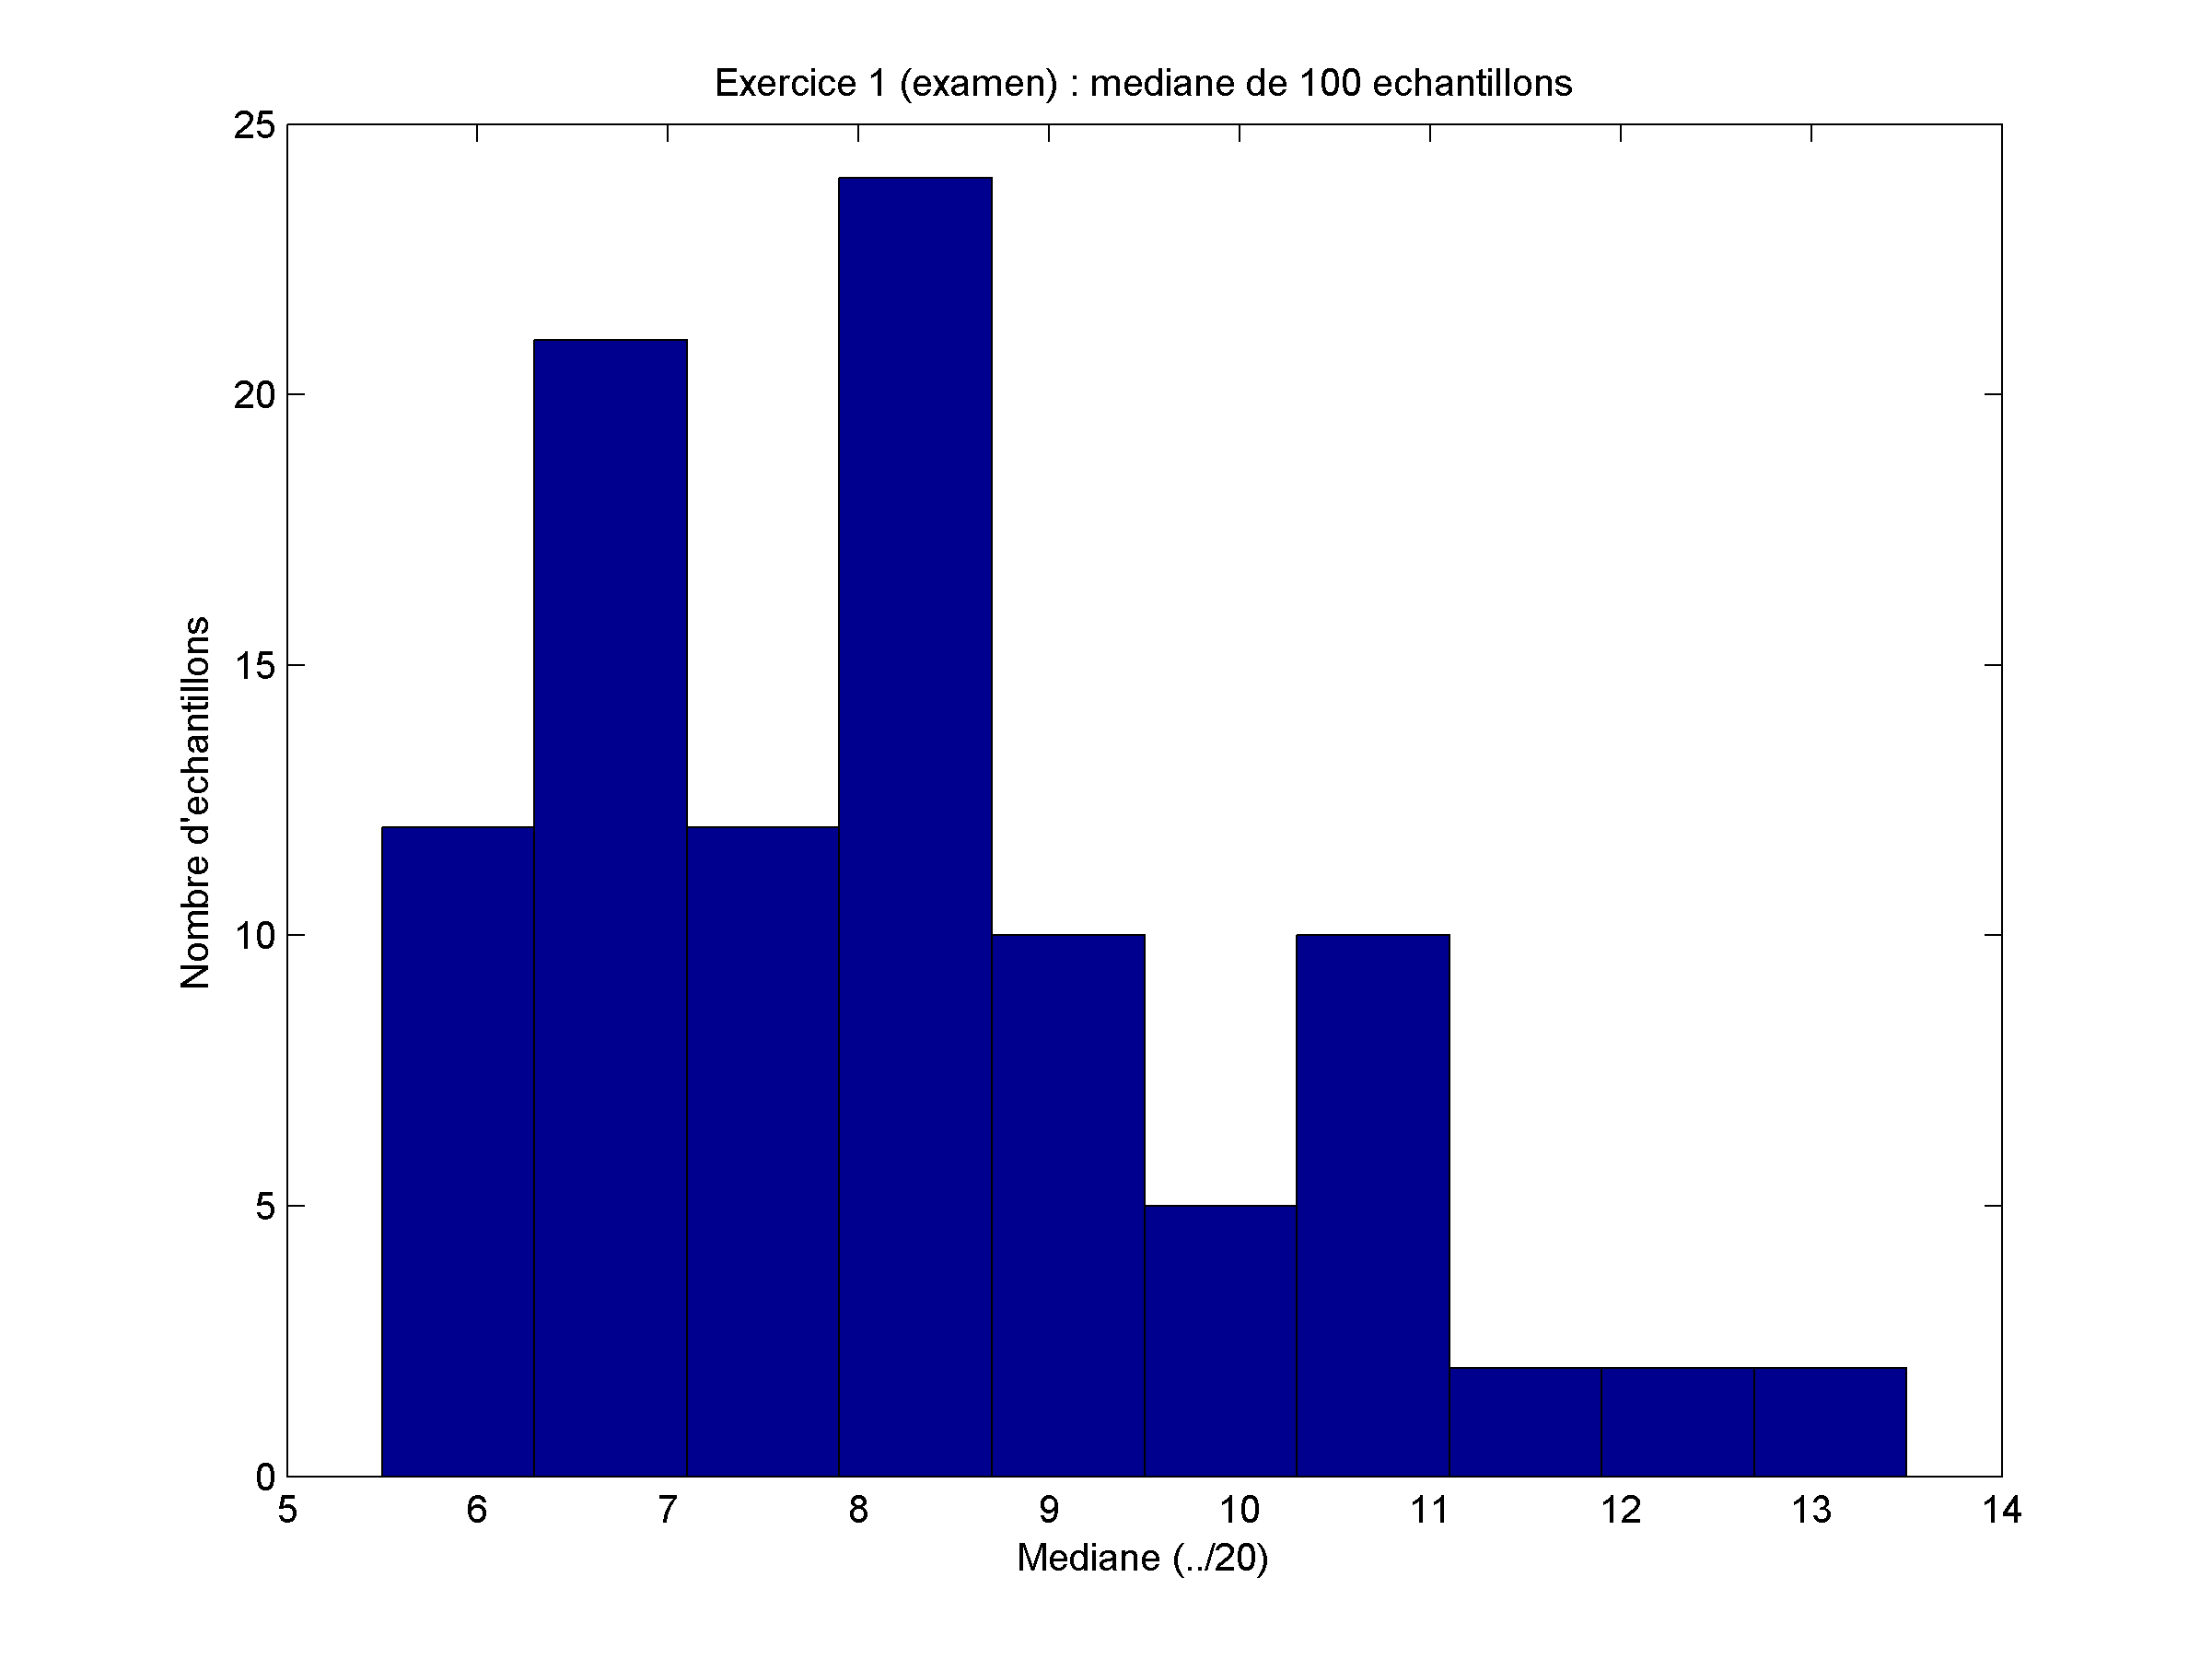
\includegraphics[scale=0.35]{q2b-mediane.png}}
	\subfigure[Écart-type]{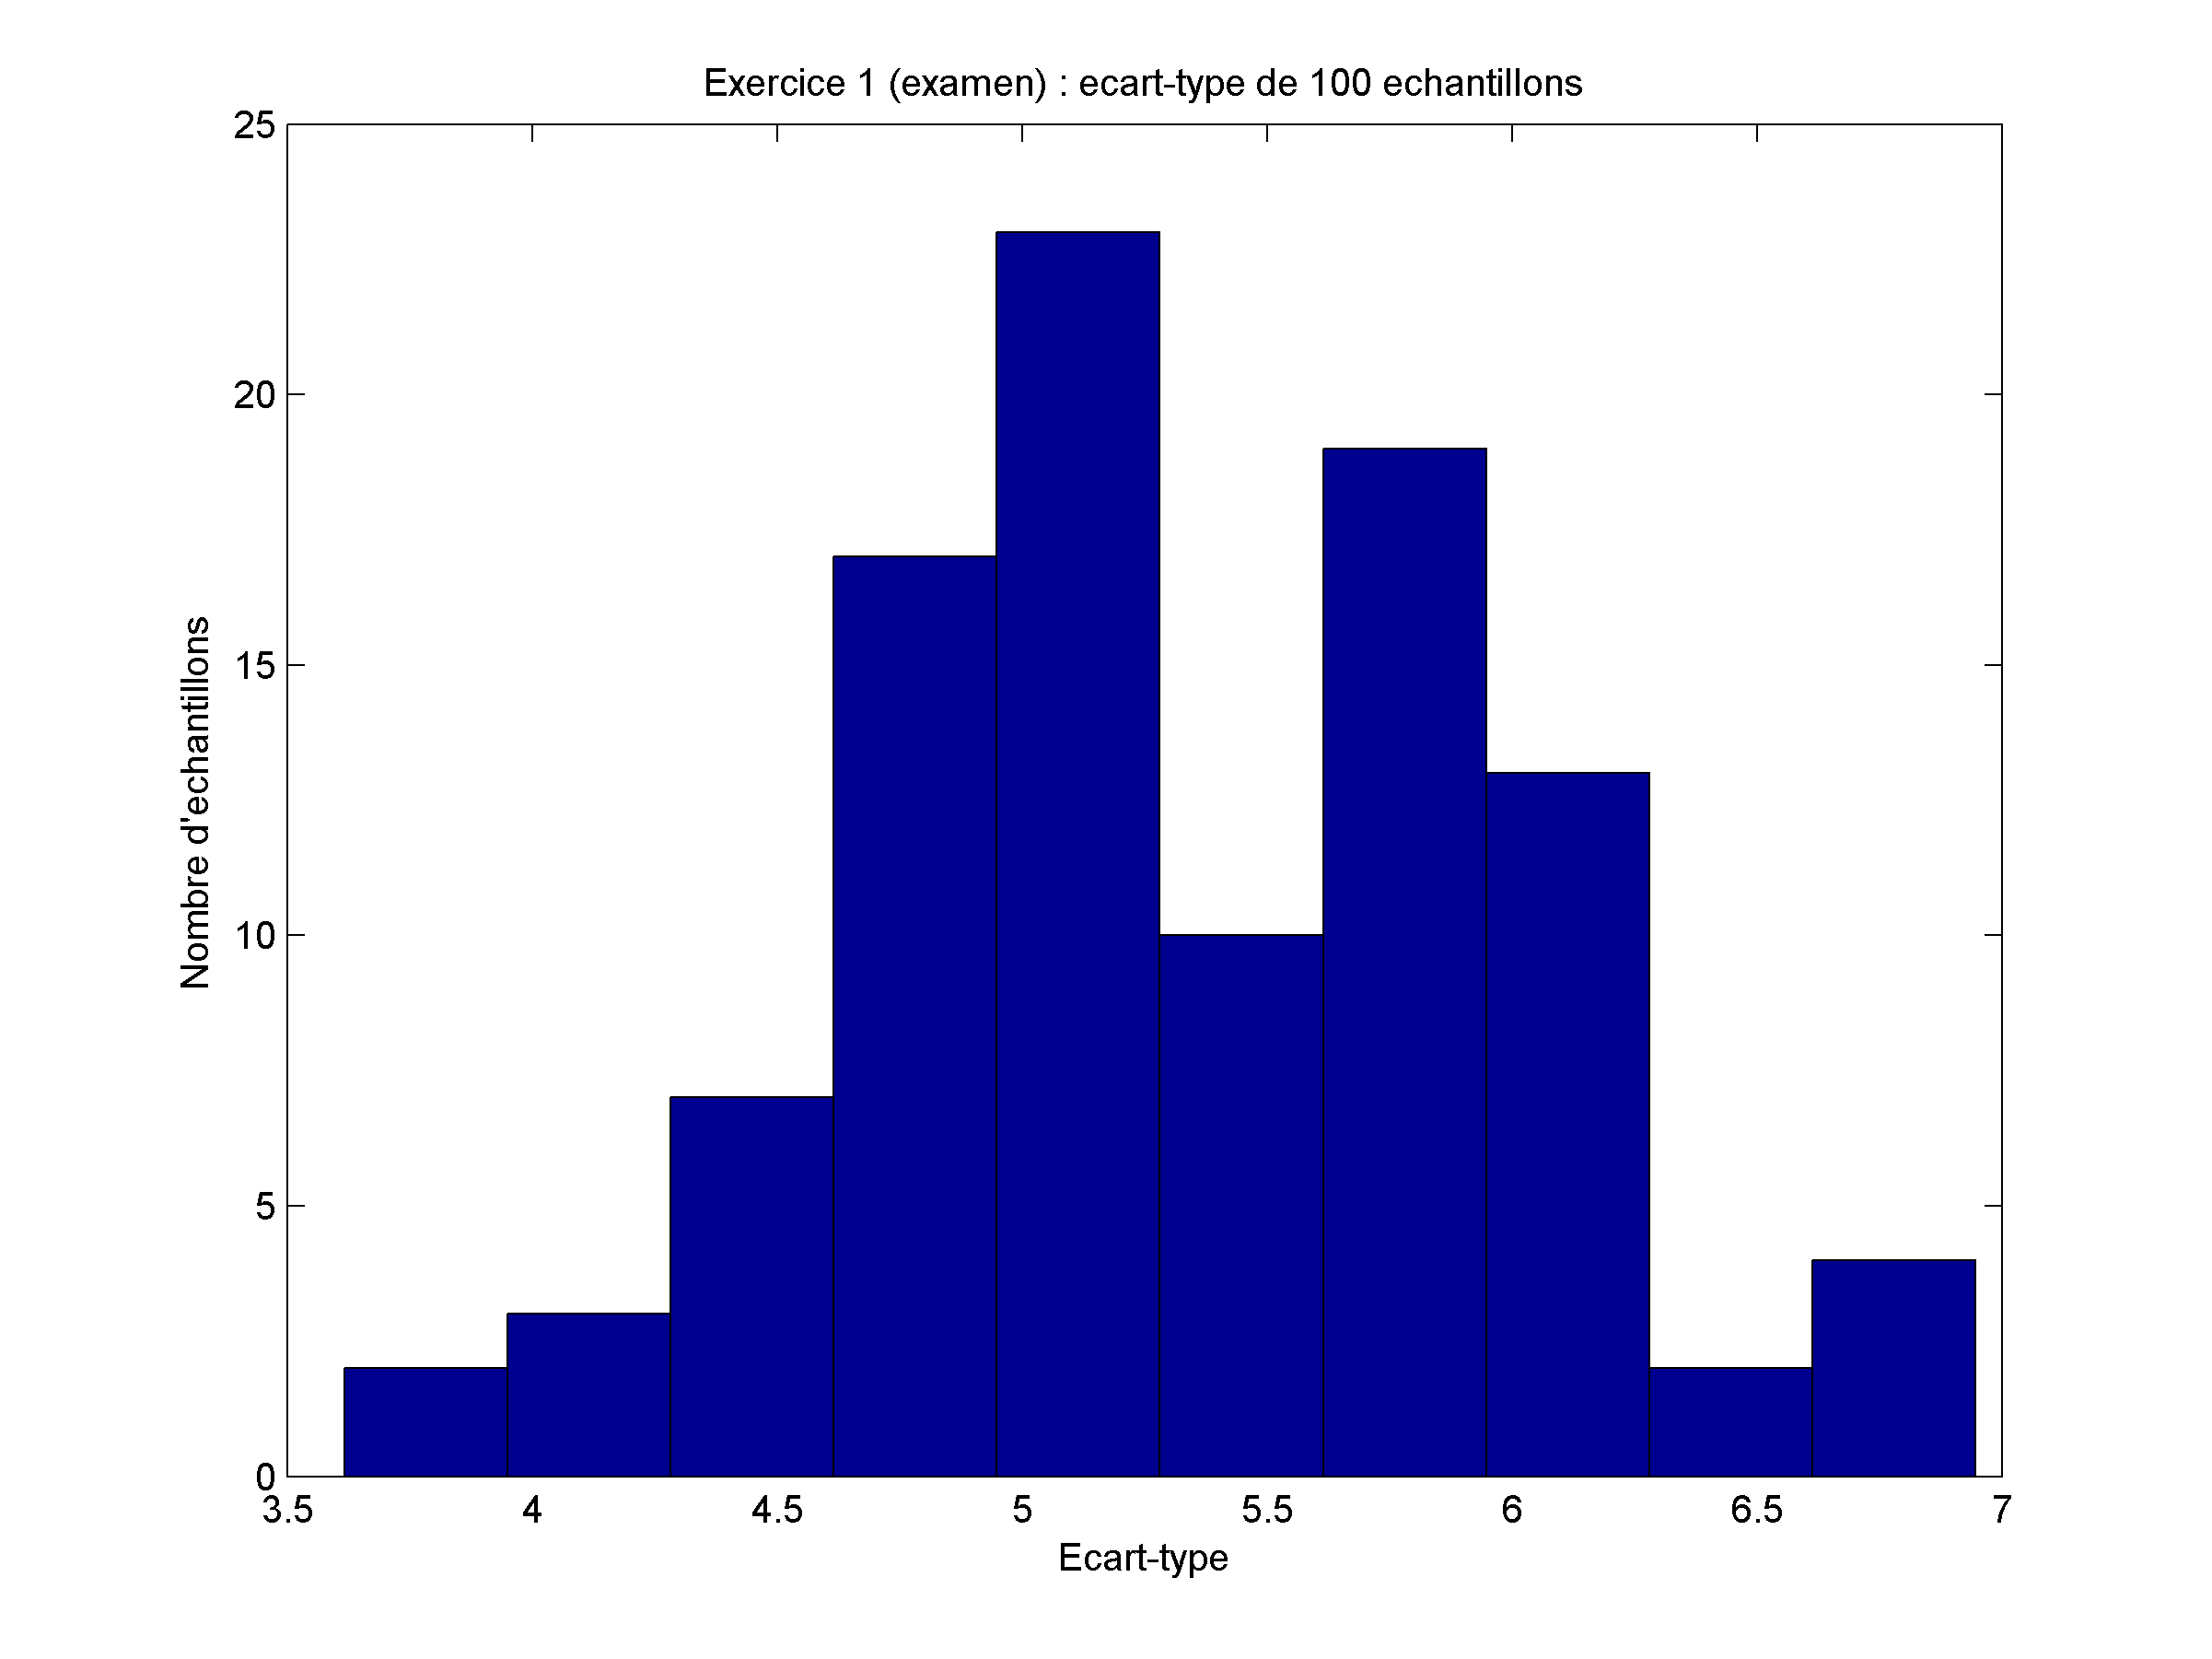
\includegraphics[scale=0.35]{q2b-std.png}}
	\caption{Calculs statistiques pour l'exercice 1 (100 échantillons)}
	\label{fig:q2b_stat_100sample}
\end{figure}

%
\begin{figure}[!h]
	\center
	\subfigure[Exercice 1]{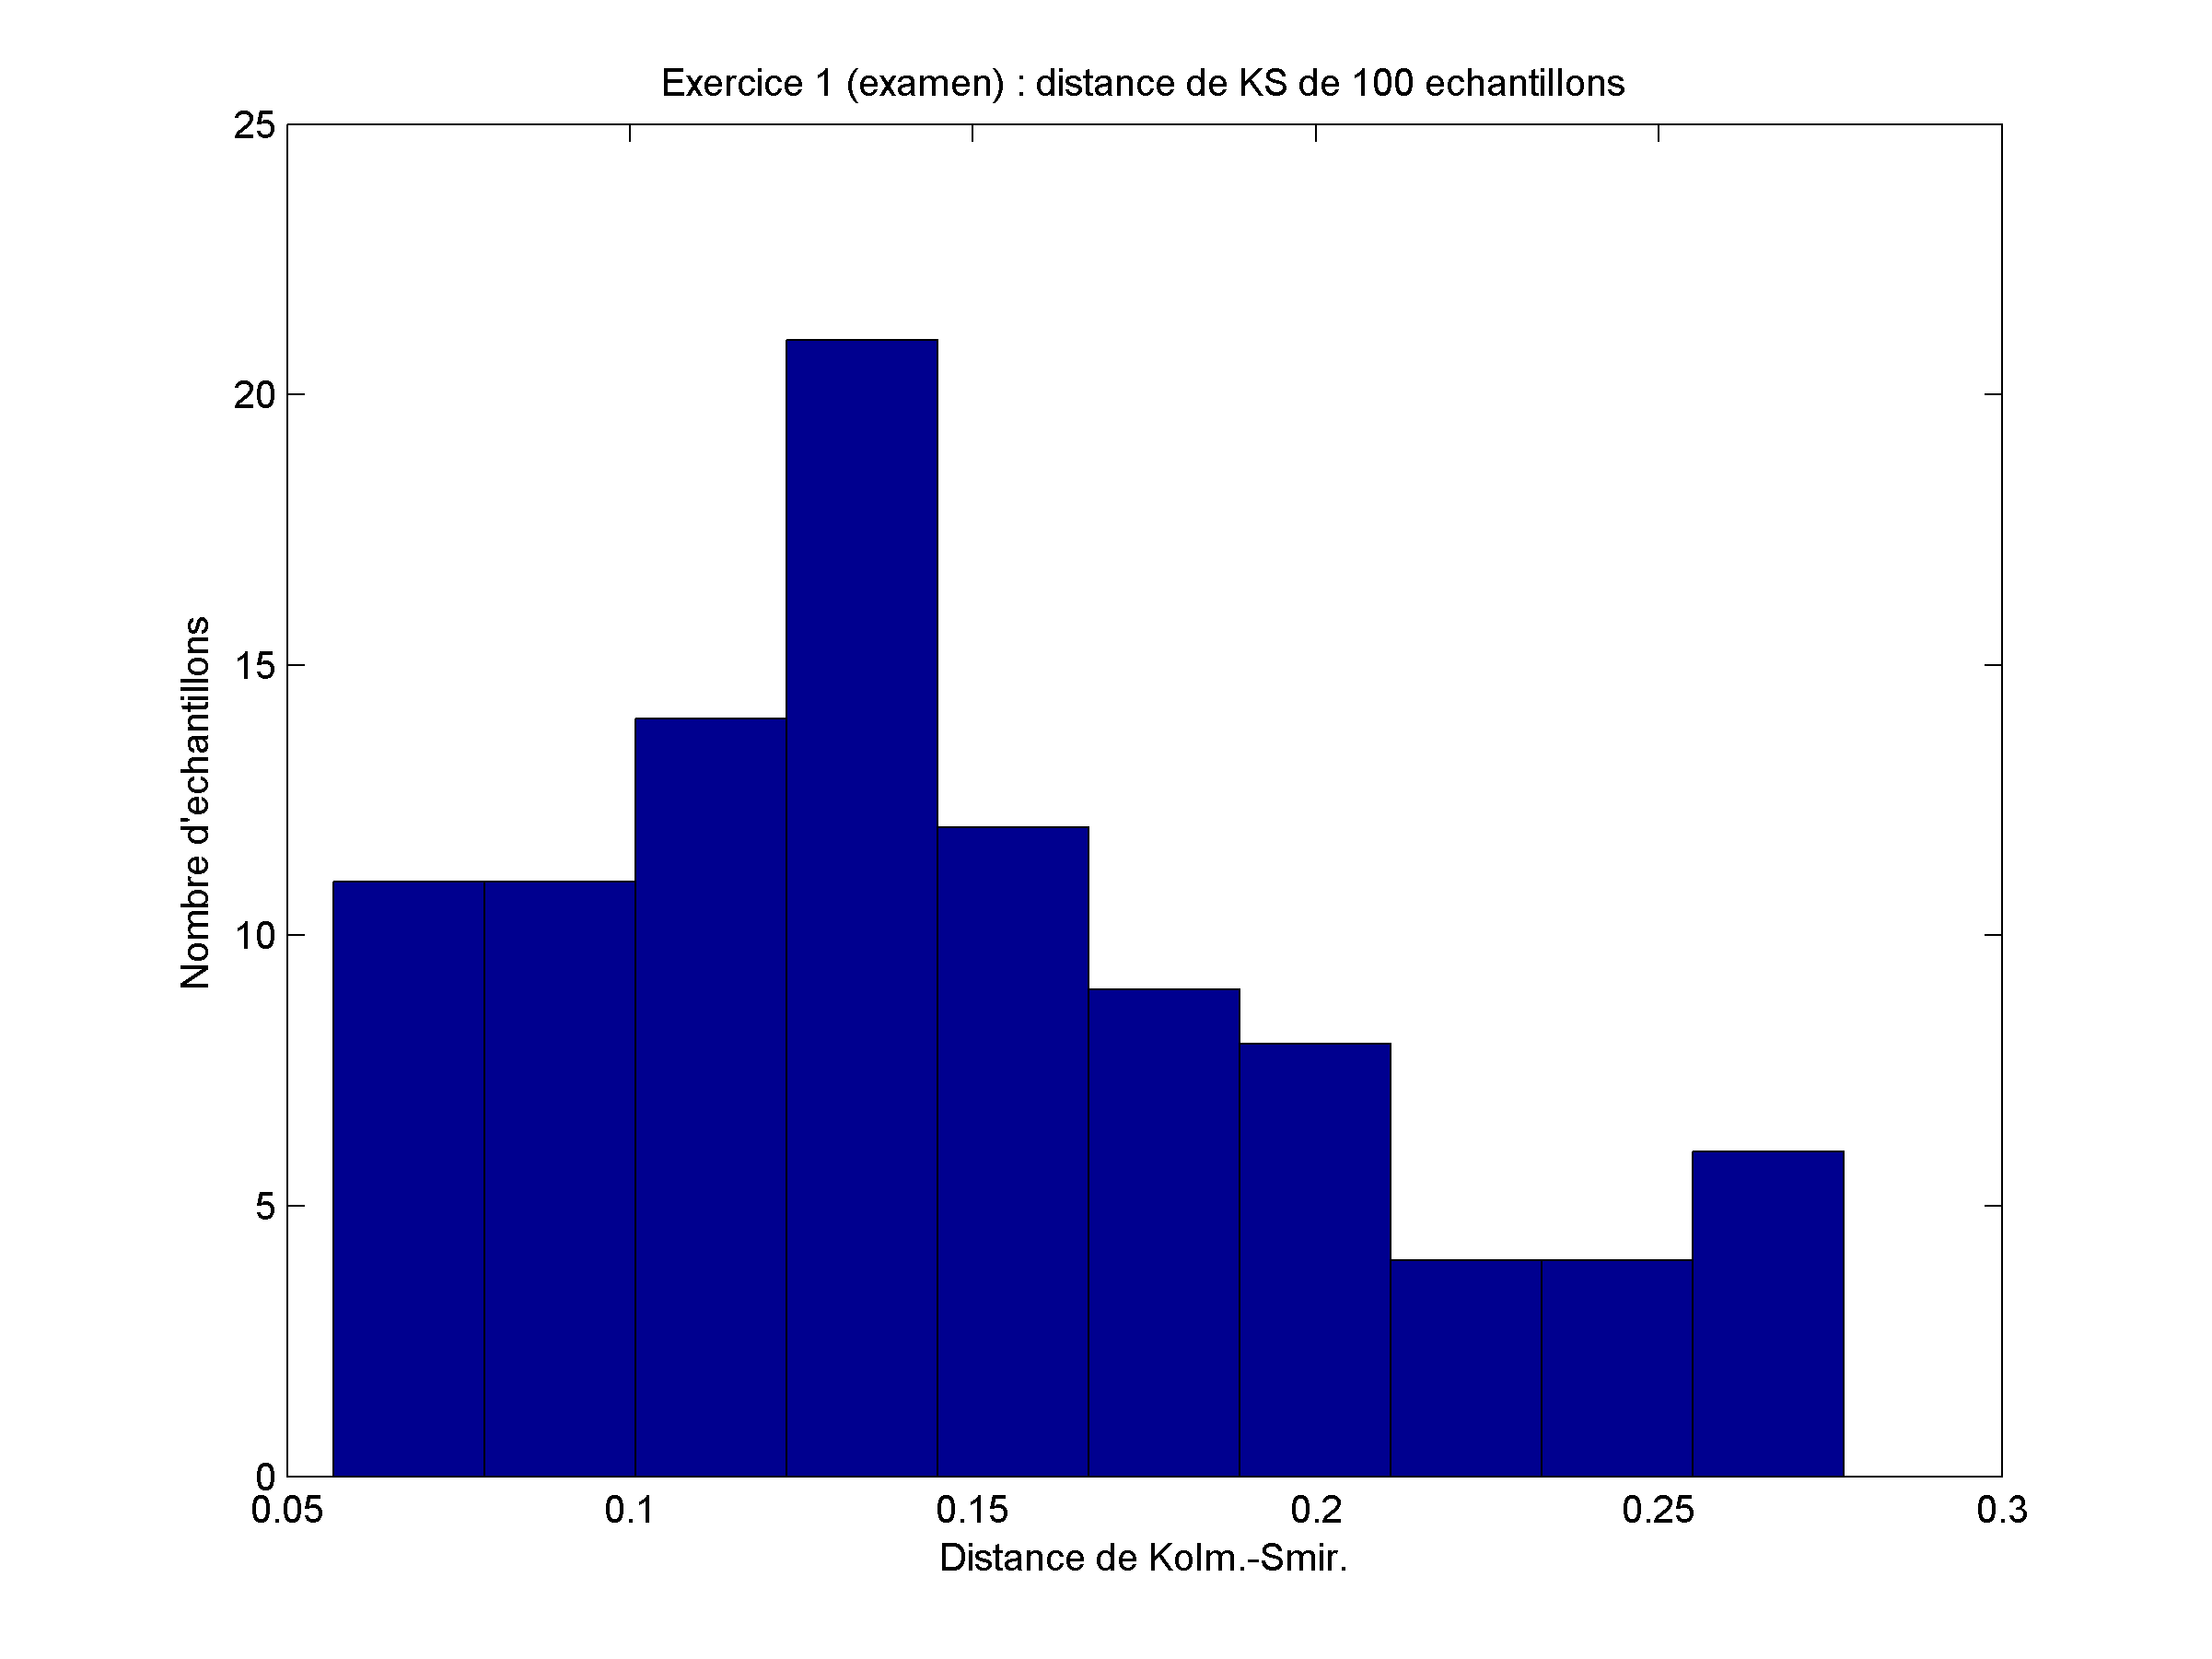
\includegraphics[scale=0.35]{q2b-ks-ex1.png}}
	\subfigure[Exercice 2]{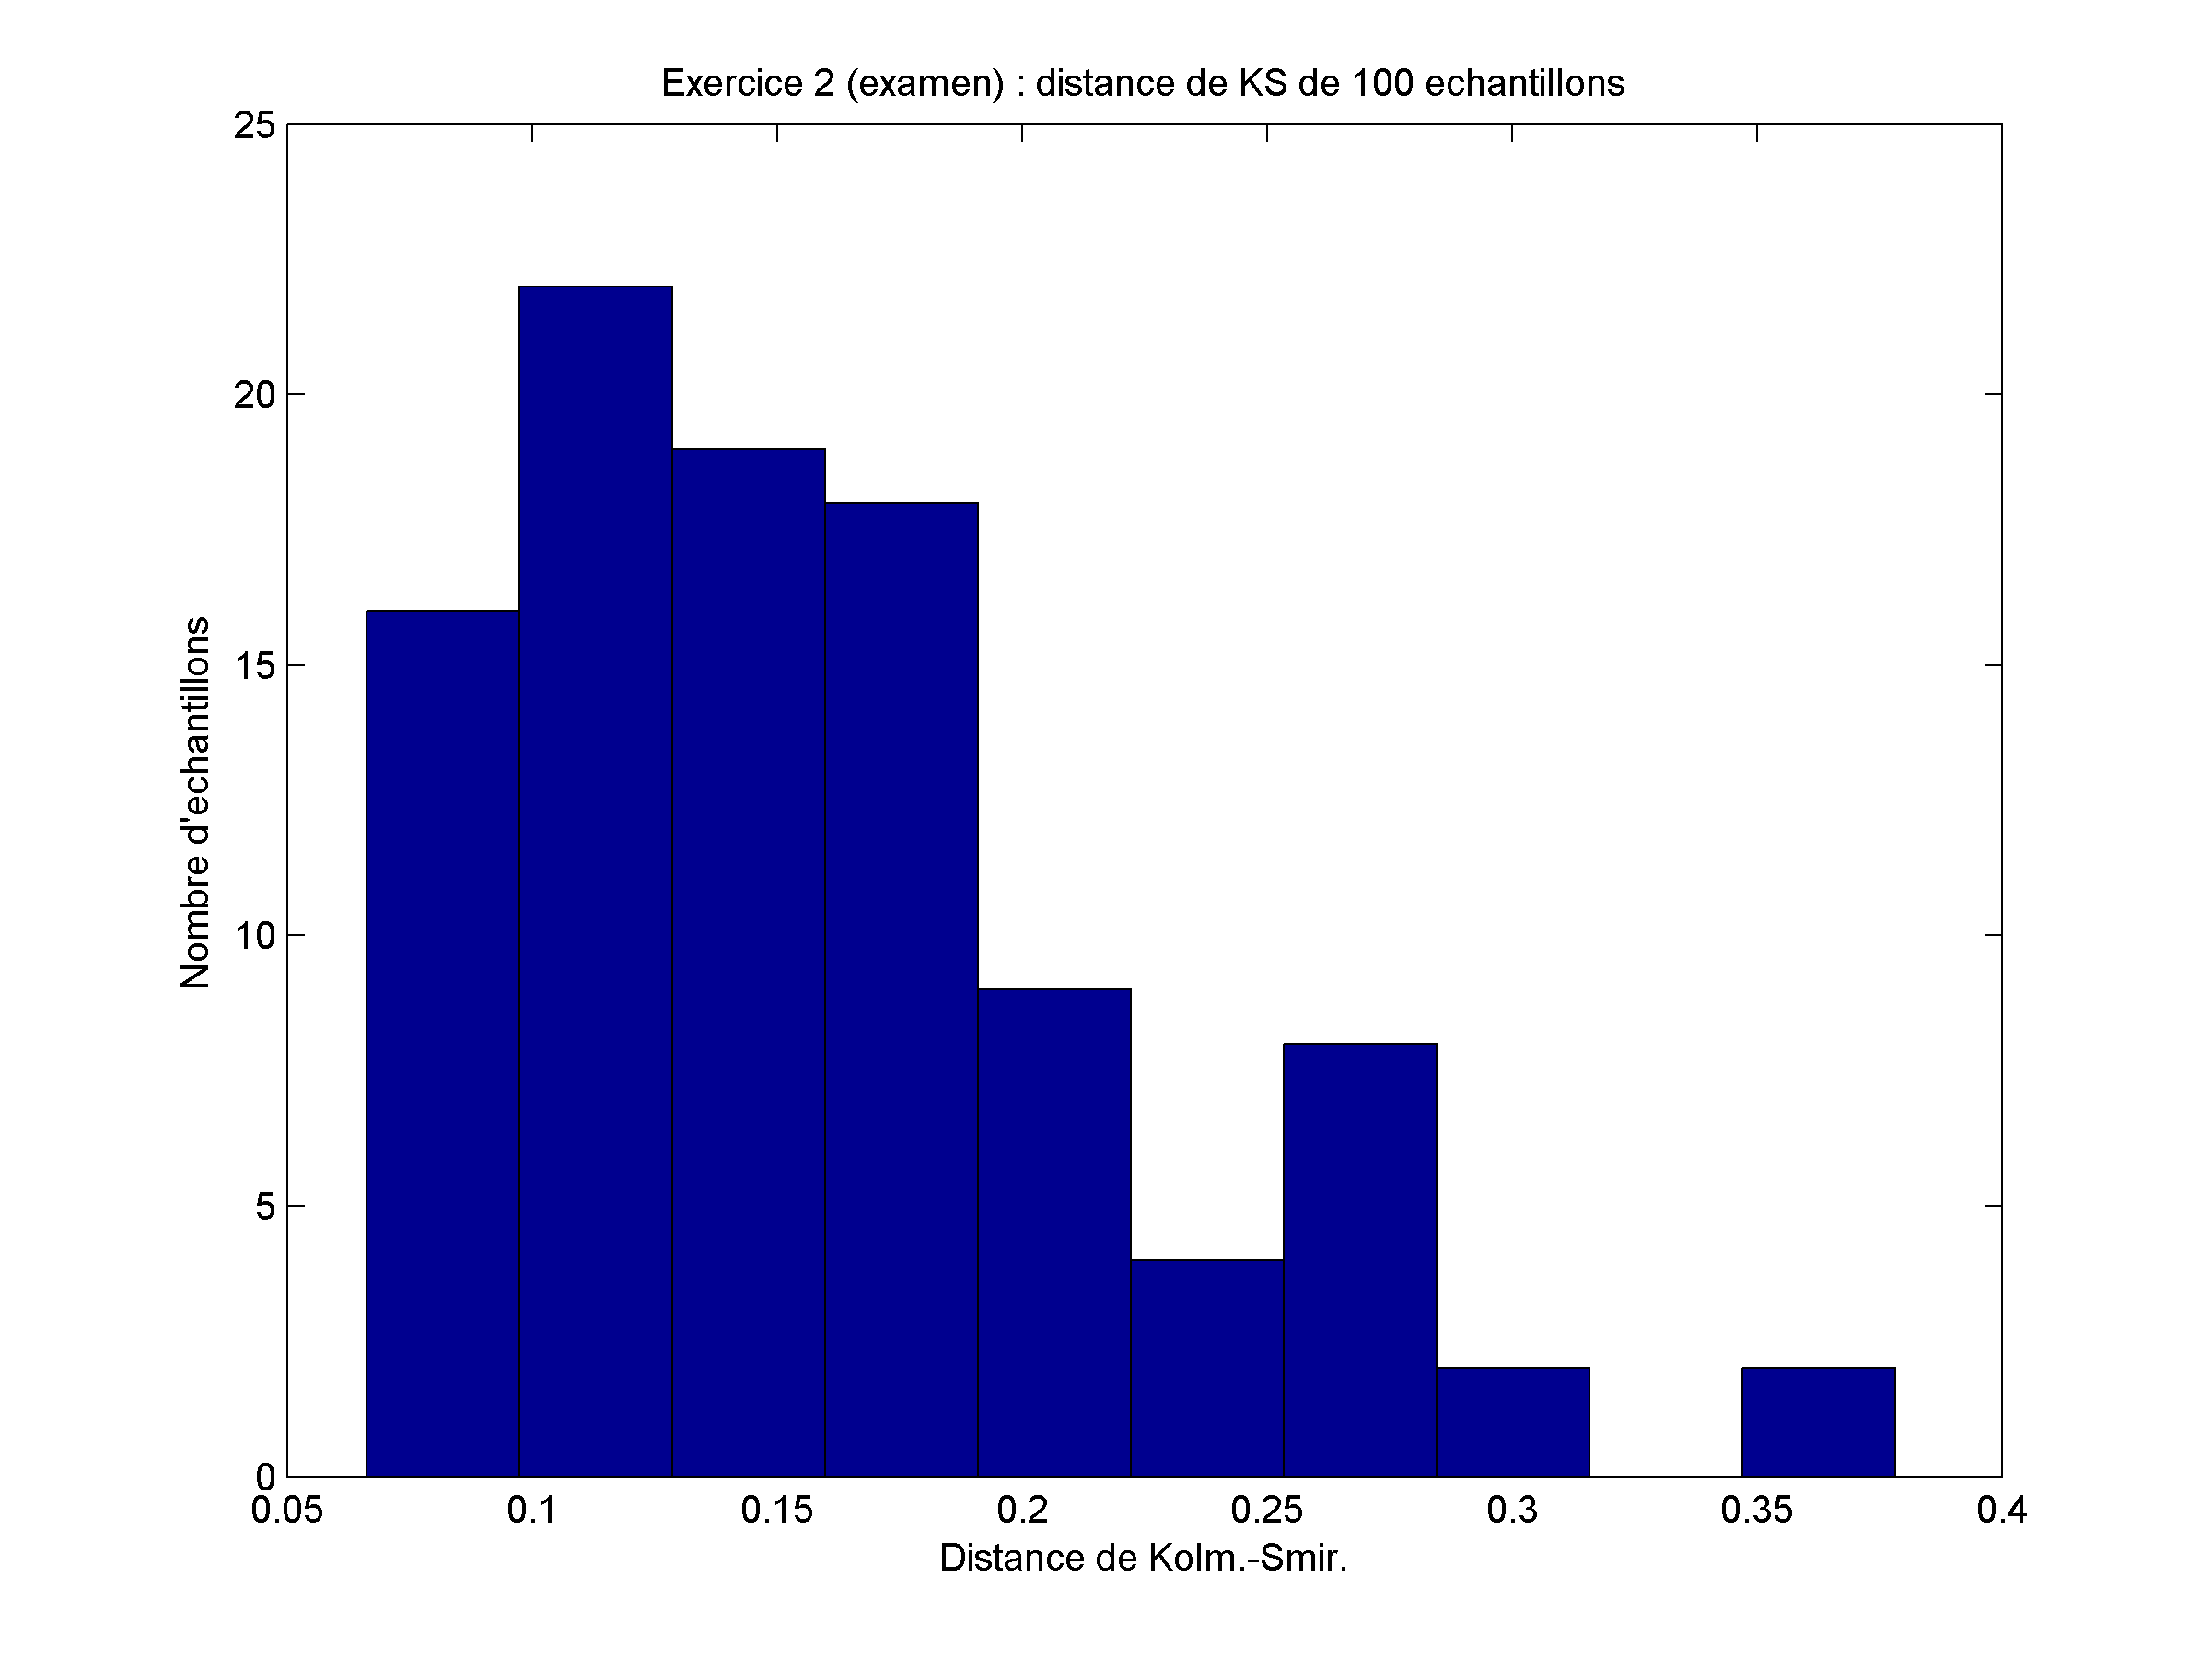
\includegraphics[scale=0.35]{q2b-ks-ex2.png}}
	\subfigure[Exercice 3]{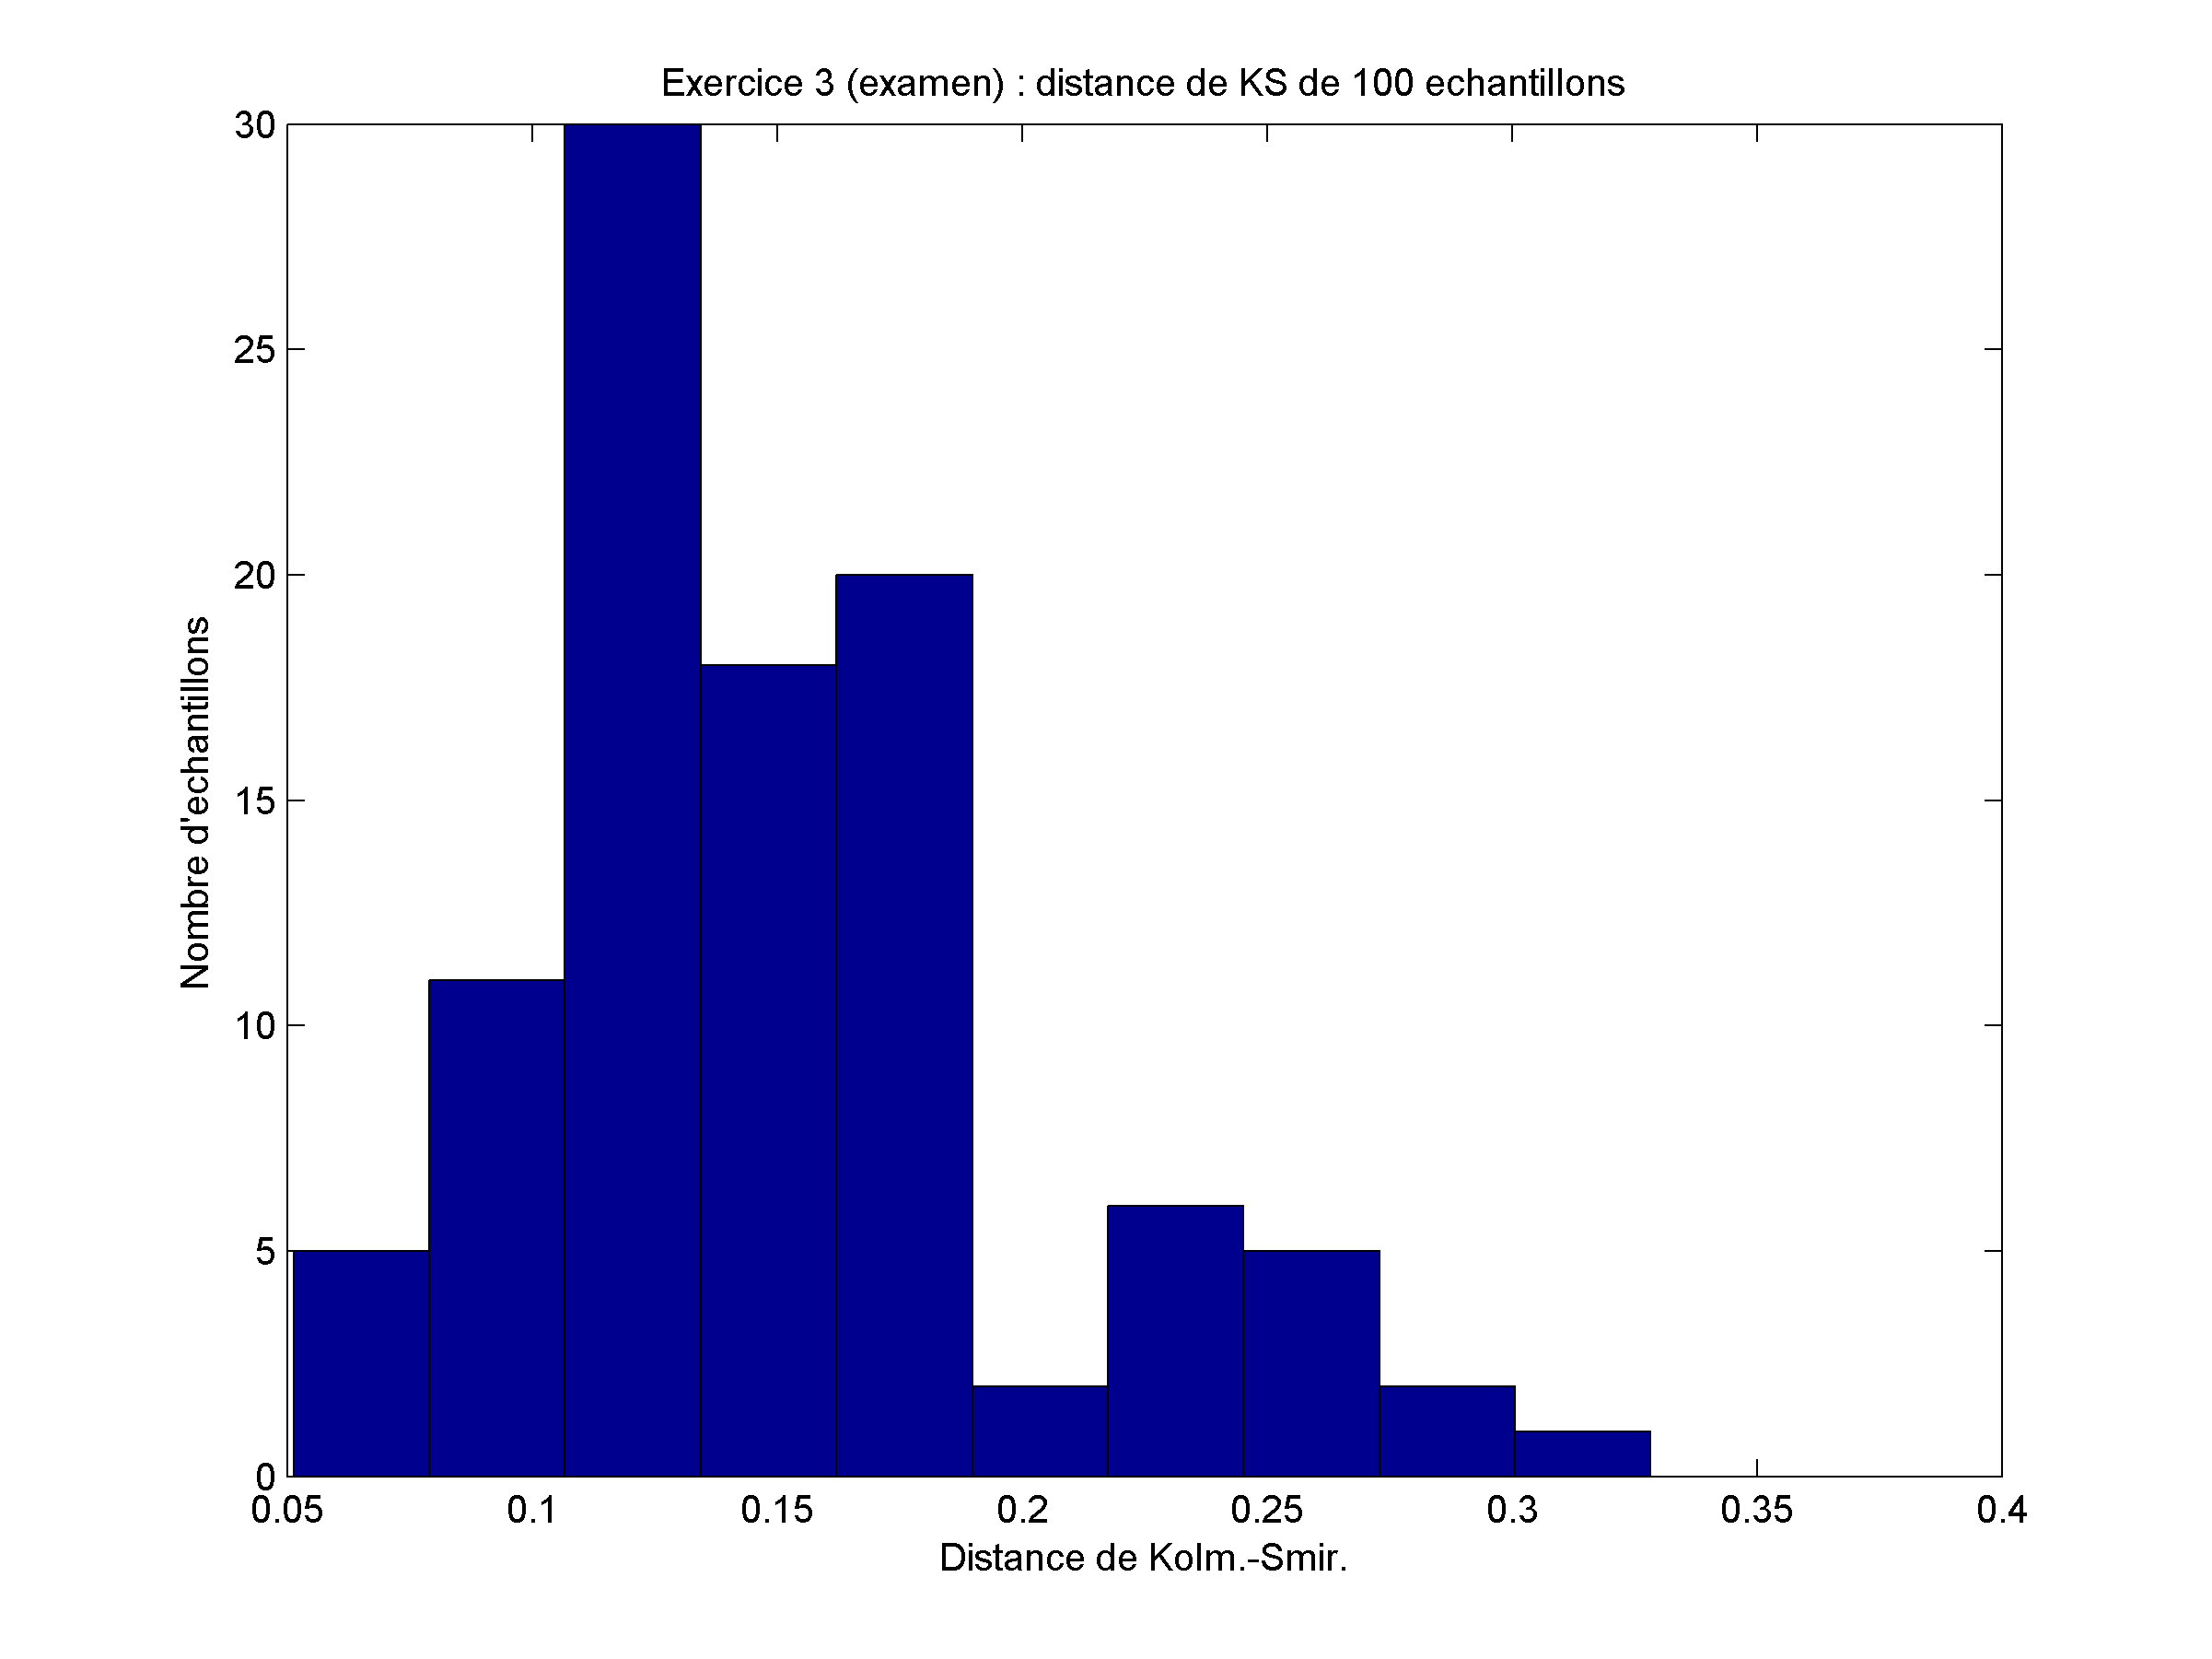
\includegraphics[scale=0.35]{q2b-ks-ex3.png}}
	\caption{Distance de Kolmogorov-Smirnov de 100 échantillons par rapport à la population}
	\label{fig:q2b_ks_100sample}
\end{figure}
%
\section{Annexe}
\subsection{Code}
\begin{lstlisting}[caption={\texttt{Question1.m}}]
clear all;
close all;

% Load data
s_score = load('stat_data.mat');
score = s_score.m;
clear s_score;
% Splitting different columns into different variables
exam_exer = score(:,8:10);
exam_theo = score(:,5:7);
exam_proj = score(:,4);
projects  = score(:,1:4);
n_students = length(score(:,1));

%% Question 1
% Point a)
figure; hist(exam_theo(:,1), 20); % theorie 1
title('Theorie : question 1');
ylabel('Nombre d''eleves');
xlabel('Points');

figure; hist(exam_theo(:,2), 20); % theorie 2
title('Theorie : question 2');
ylabel('Nombre d''eleves');
xlabel('Points');

figure; hist(exam_theo(:,3), 20); % theorie 3
title('Theorie : question 3');
ylabel('Nombre d''eleves');
xlabel('Points');

% Point b)
ex_mean   = mean(exam_exer);
ex_median = median(exam_exer);
ex_mode   = mode(exam_exer);
ex_ectype = std(exam_exer, 1);

norm_min_threshold = ex_mean - ex_ectype;
norm_max_threshold = ex_mean + ex_ectype;

n_students_normal_exer = [length(find(exam_exer(:,1) >= norm_min_threshold(1) & exam_exer(:,1) <= norm_max_threshold(1) )) ...
	length(find(exam_exer(:,2) >= norm_min_threshold(2) & exam_exer(:,2) <= norm_max_threshold(2) )) ...
	length(find(exam_exer(:,3) >= norm_min_threshold(3) & exam_exer(:,3) <= norm_max_threshold(3) ))];

% Point c)
figure; boxplot(projects(:,1));
title('Projet 1');
ylabel('Points');

figure; boxplot(projects(:,2));
title('Projet 2');
ylabel('Points');

figure; boxplot(projects(:,3));
title('Projet 3');
ylabel('Points');

figure; boxplot(exam_proj);
title('Examen : question sur le projet');
ylabel('Points');

proj_Q1 = quantile(projects, 0.25);
proj_Q3 = quantile(projects, 0.75);

min_threshold = proj_Q1 - 1.5 * (proj_Q3 - proj_Q1);
max_threshold = proj_Q3 + 1.5 * (proj_Q3 - proj_Q1);

% Finding outliers indexes
outlier_index_p1 = [find(projects(:,1) < min_threshold(1)); find(projects(:,1) > max_threshold(1))];
outlier_index_p2 = [find(projects(:,2) < min_threshold(2)); find(projects(:,2) > max_threshold(2))];
outlier_index_p3 = [find(projects(:,3) < min_threshold(3)); find(projects(:,3) > max_threshold(3))];
outlier_index_exam_p = [find(projects(:,4) < min_threshold(4)); find(projects(:,4) > max_threshold(4))];

outliers_p1 = projects(outlier_index_p1, 1).';
outliers_p2 = projects(outlier_index_p2, 2).';
outliers_p3 = projects(outlier_index_p3, 3).';
outliers_ex_proj = projects(outlier_index_exam_p, 4).'; 

clear outlier_index_p1 outlier_index_p2 outlier_index_p3 outlier_index_exam_p;

% Point d)
theo_mean = mean(exam_theo .').';
exer_mean = mean(exam_exer .').';

figure; cdfplot(theo_mean);
title('Frequence cumulee pour la moyenne des questions de theorie');
xlabel('Points (../20)');
ylabel('Frequence relative cumulee (theorie)');

figure; cdfplot(exer_mean);
title('Frequence cumulee pour la moyenne des questions d''exercice');
xlabel('Points (../20)');
ylabel('Frequence relative cumulee (exercice)');

[ecdf_theo x_ecdf_theo] = ecdf(theo_mean);
[ecdf_exer x_ecdf_exer] = ecdf(exer_mean);

%close all;
res_min = find(x_ecdf_exer >= 12, 1);
res_max = find(x_ecdf_exer <= 15, 1, 'last');
score12_15_exer = (ecdf_exer(res_max) - ecdf_exer(res_min));

res_min = find(x_ecdf_theo >= 12, 1);
res_max = find(x_ecdf_theo <= 15, 1, 'last');
score12_15_theo = (ecdf_theo(res_max) - ecdf_theo(res_min));

clear res_min res_max;
% Point e)
figure; scatter(projects(:,3), exam_proj, 4*pi, 'blue', 'fill');
title('Projet 3 et question d''examen sur le projet 3');
xlabel('Points projet 3 (../20)');
ylabel('Points question sur le projet 3 (../20)');

corr_proj3 = corrcoef(projects(:,3), exam_proj);
corr_coef_p3 = corr_proj3(1,2);

clear corr_proj3;
\end{lstlisting}
\begin{lstlisting}[caption={\texttt{Question2.m}}]
clear all;
close all;

% Load data
s_score = load('stat_data.mat');
score = s_score.m;
clear s_score;
% Splitting different columns into different variables
exam_exer = score(:,8:10);
exam_theo = score(:,5:7);
exam_proj = score(:,4);
projects  = score(:,1:4);
n_students = length(score(:,1));

%% Question 2.a
[sample_2a sample_index_2a] = datasample(score, 20);

% Question 2.a.i
ex_mean   = mean(sample_2a(:,8:10));
ex_median = median(sample_2a(:,8:10));
ex_ectype = std(sample_2a(:,8:10));

% Question 2.a.ii
figure; boxplot(sample_2a(:,1));
title('Projet 1 (sample)');
ylabel('Points');

figure; boxplot(sample_2a(:,2));
title('Projet 2 (sample)');
ylabel('Points');

figure; boxplot(sample_2a(:,3));
title('Projet 3 (sample)');
ylabel('Points');

figure; boxplot(sample_2a(:,4));
title('Examen : question sur le projet (sample)');
ylabel('Points');

% Question 2.a.iii
theo_mean_sample_2a = mean(sample_2a(:,5:7).').';
theo_mean = mean(exam_theo.').';

ks = ksdist(theo_mean_sample_2a, theo_mean);
[~, ~, ks_f] = kstest2(theo_mean_sample_2a, theo_mean);
figure; cdfplot(theo_mean_sample_2a);
figure; cdfplot(theo_mean);

%% Question 2.b
n_sample = 100;
sample_size = 20;
sample_2b = zeros(sample_size, n_sample);

for i=1:n_sample
	sample_2b(:,i) = datasample(exam_exer(:,1), sample_size);
end

% Resultat de la question 1 (population)
ex1_mean = mean(exam_exer(:,1));
ex1_median = median(exam_exer(:,1));
ex1_std = mean(exam_exer(:,1));

% Question 2.b.i
ex1_mean_s = mean(sample_2b).';

figure; hist(ex1_mean_s);
title('Exercice 1 (examen) : moyenne de 100 echantillons');
ylabel('Nombre d''echantillons');
xlabel('Moyenne (../20)');

mean_ex1_mean_s = mean(ex1_mean_s);

% Question 2.b.ii
ex1_median_s = median(sample_2b).';

figure; hist(ex1_median_s);
title('Exercice 1 (examen) : mediane de 100 echantillons');
ylabel('Nombre d''echantillons');
xlabel('Mediane (../20)');

mean_ex1_median_s = mean(ex1_median_s);

% Question 2.b.iii
ex1_std_s = std(sample_2b).';

figure; hist(ex1_std_s);
title('Exercice 1 (examen) : ecart-type de 100 echantillons');
ylabel('Nombre d''echantillons');
xlabel('Ecart-type');

mean_ex1_std_s = mean(ex1_std_s);

% Question 2.b.iv 

ks_ex1 = zeros(100,1);

for i = 1:100
	ks_ex1(i) = ksdist(exam_exer(:,1), sample_2b(:,i));
end

figure; hist(ks_ex1, 10);
title('Exercice 1 (examen) : distance de KS de 100 echantillons');
ylabel('Nombre d''echantillons');
xlabel('Distance de Kolm.-Smir.');

% Question 2.b.v

ks_ex2 = zeros(100,1);
ks_ex3 = zeros(100,1);

for i = 1:100
	[~, ~, ks_ex2(i)] = kstest2(exam_exer(:,2), datasample(exam_exer(:,2), sample_size));
	[~, ~, ks_ex3(i)] = kstest2(exam_exer(:,3), datasample(exam_exer(:,3), sample_size));
end

figure; hist(ks_ex2, 10);
title('Exercice 2 (examen) : distance de KS de 100 echantillons');
ylabel('Nombre d''echantillons');
xlabel('Distance de Kolm.-Smir.');

figure; hist(ks_ex3, 10);
title('Exercice 3 (examen) : distance de KS de 100 echantillons');
ylabel('Nombre d''echantillons');
xlabel('Distance de Kolm.-Smir.');
\end{lstlisting}
\begin{lstlisting}[caption={\texttt{datasample.m}}]
function [sample index_perm] = datasample(data, k)
	% datasample(data, k)
	%	This function returns a random sample from the matrix $data$.
	%	It randomly selects $k$ lines in the matrix. 
	% 
	%	/!\ $k$ must be less than the numbers of row in $data$
	%	
	%	PARAMETERS :
	%		- data : the matrix from which a sample must be extracted
	%		- k : the size of the sample
	%
	%	RETURN :
	%		- sample : the sample extracted
	%		- index_perm : the (row) indexes of the values extracted in $data$ 

	[len_x ~] = size(data);

	if(k >= len_x)
		error('The sample size ''k'' must be less than or equal to the number of line in the matrix');
	else
		index_perm = randi(len_x, k, 1);
		index_perm = sort(index_perm);
		sample = data(index_perm,:);
	end
end
\end{lstlisting}
\end{document}